\RequirePackage{silence} % :-\
    \WarningFilter{scrreprt}{Usage of package `titlesec'}
    %\WarningFilter{scrreprt}{Activating an ugly workaround}
    \WarningFilter{titlesec}{Non standard sectioning command detected}
\documentclass[ twoside,openright,titlepage,numbers=noenddot,%1headlines,
                headinclude,footinclude,cleardoublepage=empty,abstract=on,
                BCOR=5mm,paper=a4,fontsize=11pt
                ]{scrreprt}

%********************************************************************
% Note: Make all your adjustments in here
%*******************************************************
% ****************************************************************************************************
% classicthesis-config.tex
% formerly known as loadpackages.sty, classicthesis-ldpkg.sty, and classicthesis-preamble.sty
% Use it at the beginning of your ClassicThesis.tex, or as a LaTeX Preamble
% in your ClassicThesis.{tex,lyx} with % ****************************************************************************************************
% classicthesis-config.tex
% formerly known as loadpackages.sty, classicthesis-ldpkg.sty, and classicthesis-preamble.sty
% Use it at the beginning of your ClassicThesis.tex, or as a LaTeX Preamble
% in your ClassicThesis.{tex,lyx} with % ****************************************************************************************************
% classicthesis-config.tex
% formerly known as loadpackages.sty, classicthesis-ldpkg.sty, and classicthesis-preamble.sty
% Use it at the beginning of your ClassicThesis.tex, or as a LaTeX Preamble
% in your ClassicThesis.{tex,lyx} with \input{classicthesis-config}
% ****************************************************************************************************
% If you like the classicthesis, then I would appreciate a postcard.
% My address can be found in the file ClassicThesis.pdf. A collection
% of the postcards I received so far is available online at
% http://postcards.miede.de
% ****************************************************************************************************


% ****************************************************************************************************
% 0. Set the encoding of your files. UTF-8 is the only sensible encoding nowadays. If you can't read
% äöüßáéçèê∂åëæƒÏ€ then change the encoding setting in your editor, not the line below. If your editor
% does not support utf8 use another editor!
% ****************************************************************************************************
\PassOptionsToPackage{utf8}{inputenc}
  \usepackage{inputenc}

\PassOptionsToPackage{T1}{fontenc} % T2A for cyrillics
  \usepackage{fontenc}


% ****************************************************************************************************
% 1. Configure classicthesis for your needs here, e.g., remove "drafting" below
% in order to deactivate the time-stamp on the pages
% (see ClassicThesis.pdf for more information):
% ****************************************************************************************************
\PassOptionsToPackage{
  drafting=false,    % print version information on the bottom of the pages
  tocaligned=false, % the left column of the toc will be aligned (no indentation)
  dottedtoc=false,  % page numbers in ToC flushed right
  eulerchapternumbers=true, % use AMS Euler for chapter font (otherwise Palatino)
  linedheaders=false,       % chaper headers will have line above and beneath
  floatperchapter=true,     % numbering per chapter for all floats (i.e., Figure 1.1)
  eulermath=false,  % use awesome Euler fonts for mathematical formulae (only with pdfLaTeX)
  beramono=true,    % toggle a nice monospaced font (w/ bold)
  palatino=true,    % deactivate standard font for loading another one, see the last section at the end of this file for suggestions
  style=classicthesis % classicthesis, arsclassica
}{classicthesis}


% ****************************************************************************************************
% 2. Personal data and user ad-hoc commands (insert your own data here)
% ****************************************************************************************************
\newcommand{\myTitle}{Machine Learning in a Nutshell\xspace}
\newcommand{\mySubtitle}{An Homage to The Elements of Typographic Style\xspace}
\newcommand{\myDegree}{Doktor-Ingenieur (Dr.-Ing.)\xspace}
\newcommand{\myName}{Thimo Preis\xspace}
\newcommand{\myProf}{Put name here\xspace}
\newcommand{\myOtherProf}{Put name here\xspace}
\newcommand{\mySupervisor}{Put name here\xspace}
\newcommand{\myFaculty}{Put data here\xspace}
\newcommand{\myDepartment}{Put data here\xspace}
\newcommand{\myUni}{Put data here\xspace}
\newcommand{\myLocation}{Saarbrücken\xspace}
\newcommand{\myTime}{ \today \xspace}
\newcommand{\myVersion}{\classicthesis}
\newcommand{\myEmail}{\href{mailto:thimo.preis@posteo.de}{thimo.preis@posteo.de}}
% ********************************************************************
% Setup, finetuning, and useful commands
% ********************************************************************
\providecommand{\mLyX}{L\kern-.1667em\lower.25em\hbox{Y}\kern-.125emX\@}
\newcommand{\ie}{i.\,e.}
\newcommand{\Ie}{I.\,e.}
\newcommand{\eg}{e.\,g.}
\newcommand{\Eg}{E.\,g.}
% ****************************************************************************************************


% ****************************************************************************************************
% 3. Loading some handy packages
% ****************************************************************************************************
% ********************************************************************
% Packages with options that might require adjustments
% ********************************************************************
\PassOptionsToPackage{ngerman,american, british}{babel} % change this to your language(s), main language last
% Spanish languages need extra options in order to work with this template
%\PassOptionsToPackage{spanish,es-lcroman}{babel}
    \usepackage{babel}

\usepackage{csquotes}
\PassOptionsToPackage{%
  %backend=biber,bibencoding=utf8, %instead of bibtex
  backend=bibtex8,bibencoding=ascii,%
  language=auto,%
  style=numeric-comp,%
  %style=authoryear-comp, % Author 1999, 2010
  %bibstyle=authoryear,dashed=false, % dashed: substitute rep. author with ---
  sorting=nyt, % name, year, title
  maxbibnames=10, % default: 3, et al.
  %backref=true,%
  natbib=true % natbib compatibility mode (\citep and \citet still work)
}{biblatex}
    \usepackage{biblatex}

\PassOptionsToPackage{fleqn}{amsmath}       % math environments and more by the AMS
  \usepackage{amsmath}

% ********************************************************************
% General useful packages
% ********************************************************************
\usepackage{graphicx} %
\usepackage{scrhack} % fix warnings when using KOMA with listings package
\usepackage{xspace} % to get the spacing after macros right
\PassOptionsToPackage{printonlyused,smaller}{acronym}
  \usepackage{acronym} % nice macros for handling all acronyms in the thesis
  %\renewcommand{\bflabel}[1]{{#1}\hfill} % fix the list of acronyms --> no longer working
  %\renewcommand*{\acsfont}[1]{\textsc{#1}}
  %\renewcommand*{\aclabelfont}[1]{\acsfont{#1}}
  %\def\bflabel#1{{#1\hfill}}
  \def\bflabel#1{{\acsfont{#1}\hfill}}
  \def\aclabelfont#1{\acsfont{#1}}
% ****************************************************************************************************
%\usepackage{pgfplots} % External TikZ/PGF support (thanks to Andreas Nautsch)
%\usetikzlibrary{external}
%\tikzexternalize[mode=list and make, prefix=ext-tikz/]
% ****************************************************************************************************


% ****************************************************************************************************
% 4. Setup floats: tables, (sub)figures, and captions
% ****************************************************************************************************
\usepackage{tabularx} % better tables
  \setlength{\extrarowheight}{3pt} % increase table row height
\newcommand{\tableheadline}[1]{\multicolumn{1}{l}{\spacedlowsmallcaps{#1}}}
\newcommand{\myfloatalign}{\centering} % to be used with each float for alignment
\usepackage{subfig}
% ****************************************************************************************************


% ****************************************************************************************************
% 5. Setup code listings
% ****************************************************************************************************
\usepackage{listings}
%\lstset{emph={trueIndex,root},emphstyle=\color{BlueViolet}}%\underbar} % for special keywords
\lstset{language=[LaTeX]Tex,%C++,
  morekeywords={PassOptionsToPackage,selectlanguage},
  keywordstyle=\color{RoyalBlue},%\bfseries,
  basicstyle=\small\ttfamily,
  %identifierstyle=\color{NavyBlue},
  commentstyle=\color{Green}\ttfamily,
  stringstyle=\rmfamily,
  numbers=none,%left,%
  numberstyle=\scriptsize,%\tiny
  stepnumber=5,
  numbersep=8pt,
  showstringspaces=false,
  breaklines=true,
  %frameround=ftff,
  %frame=single,
  belowcaptionskip=.75\baselineskip
  %frame=L
}
% ****************************************************************************************************




% ****************************************************************************************************
% 6. Last calls before the bar closes
% ****************************************************************************************************
% ********************************************************************
% Her Majesty herself
% ********************************************************************
\usepackage{classicthesis}


% ********************************************************************
% Fine-tune hyperreferences (hyperref should be called last)
% ********************************************************************
\hypersetup{%
  %draft, % hyperref's draft mode, for printing see below
  colorlinks=true, linktocpage=true, pdfstartpage=3, pdfstartview=FitV,%
  % uncomment the following line if you want to have black links (e.g., for printing)
  %colorlinks=false, linktocpage=false, pdfstartpage=3, pdfstartview=FitV, pdfborder={0 0 0},%
  breaklinks=true, pageanchor=true,%
  pdfpagemode=UseNone, %
  % pdfpagemode=UseOutlines,%
  plainpages=false, bookmarksnumbered, bookmarksopen=true, bookmarksopenlevel=1,%
  hypertexnames=true, pdfhighlight=/O,%nesting=true,%frenchlinks,%
  urlcolor=CTurl, linkcolor=CTlink, citecolor=CTcitation, %pagecolor=RoyalBlue,%
  %urlcolor=Black, linkcolor=Black, citecolor=Black, %pagecolor=Black,%
  pdftitle={\myTitle},%
  pdfauthor={\textcopyright\ \myName, \myUni, \myFaculty},%
  pdfsubject={},%
  pdfkeywords={},%
  pdfcreator={pdfLaTeX},%
  pdfproducer={LaTeX with hyperref and classicthesis}%
}


% ********************************************************************
% Setup autoreferences (hyperref and babel)
% ********************************************************************
% There are some issues regarding autorefnames
% http://www.tex.ac.uk/cgi-bin/texfaq2html?label=latexwords
% you have to redefine the macros for the
% language you use, e.g., american, ngerman
% (as chosen when loading babel/AtBeginDocument)
% ********************************************************************
\makeatletter
\@ifpackageloaded{babel}%
  {%
    \addto\extrasamerican{%
      \renewcommand*{\figureautorefname}{Figure}%
      \renewcommand*{\tableautorefname}{Table}%
      \renewcommand*{\partautorefname}{Part}%
      \renewcommand*{\chapterautorefname}{Chapter}%
      \renewcommand*{\sectionautorefname}{Section}%
      \renewcommand*{\subsectionautorefname}{Section}%
      \renewcommand*{\subsubsectionautorefname}{Section}%
    }%
    \addto\extrasngerman{%
      \renewcommand*{\paragraphautorefname}{Absatz}%
      \renewcommand*{\subparagraphautorefname}{Unterabsatz}%
      \renewcommand*{\footnoteautorefname}{Fu\"snote}%
      \renewcommand*{\FancyVerbLineautorefname}{Zeile}%
      \renewcommand*{\theoremautorefname}{Theorem}%
      \renewcommand*{\appendixautorefname}{Anhang}%
      \renewcommand*{\equationautorefname}{Gleichung}%
      \renewcommand*{\itemautorefname}{Punkt}%
    }%
      % Fix to getting autorefs for subfigures right (thanks to Belinda Vogt for changing the definition)
      \providecommand{\subfigureautorefname}{\figureautorefname}%
    }{\relax}
\makeatother


% ********************************************************************
% Development Stuff
% ********************************************************************
\listfiles
%\PassOptionsToPackage{l2tabu,orthodox,abort}{nag}
%  \usepackage{nag}
%\PassOptionsToPackage{warning, all}{onlyamsmath}
%  \usepackage{onlyamsmath}


% ****************************************************************************************************
% 7. Further adjustments (experimental)
% ****************************************************************************************************
% ********************************************************************
% Changing the text area
% ********************************************************************
%\areaset[current]{312pt}{761pt} % 686 (factor 2.2) + 33 head + 42 head \the\footskip
%\setlength{\marginparwidth}{7em}%
%\setlength{\marginparsep}{2em}%

% ********************************************************************
% Using different fonts
% ********************************************************************
%\usepackage[oldstylenums]{kpfonts} % oldstyle notextcomp
% \usepackage[osf]{libertine}
%\usepackage[light,condensed,math]{iwona}
%\renewcommand{\sfdefault}{iwona}
%\usepackage{lmodern} % <-- no osf support :-(
%\usepackage{cfr-lm} %
%\usepackage[urw-garamond]{mathdesign} <-- no osf support :-(
%\usepackage[default,osfigures]{opensans} % scale=0.95
%\usepackage[sfdefault]{FiraSans}
% \usepackage[opticals,mathlf]{MinionPro} % onlytext
% ********************************************************************
%\usepackage[largesc,osf]{newpxtext}
%\linespread{1.05} % a bit more for Palatino
% Used to fix these:
% https://bitbucket.org/amiede/classicthesis/issues/139/italics-in-pallatino-capitals-chapter
% https://bitbucket.org/amiede/classicthesis/issues/45/problema-testatine-su-classicthesis-style
% ********************************************************************
% ****************************************************************************************************

% ****************************************************************************************************
% If you like the classicthesis, then I would appreciate a postcard.
% My address can be found in the file ClassicThesis.pdf. A collection
% of the postcards I received so far is available online at
% http://postcards.miede.de
% ****************************************************************************************************


% ****************************************************************************************************
% 0. Set the encoding of your files. UTF-8 is the only sensible encoding nowadays. If you can't read
% äöüßáéçèê∂åëæƒÏ€ then change the encoding setting in your editor, not the line below. If your editor
% does not support utf8 use another editor!
% ****************************************************************************************************
\PassOptionsToPackage{utf8}{inputenc}
  \usepackage{inputenc}

\PassOptionsToPackage{T1}{fontenc} % T2A for cyrillics
  \usepackage{fontenc}


% ****************************************************************************************************
% 1. Configure classicthesis for your needs here, e.g., remove "drafting" below
% in order to deactivate the time-stamp on the pages
% (see ClassicThesis.pdf for more information):
% ****************************************************************************************************
\PassOptionsToPackage{
  drafting=false,    % print version information on the bottom of the pages
  tocaligned=false, % the left column of the toc will be aligned (no indentation)
  dottedtoc=false,  % page numbers in ToC flushed right
  eulerchapternumbers=true, % use AMS Euler for chapter font (otherwise Palatino)
  linedheaders=false,       % chaper headers will have line above and beneath
  floatperchapter=true,     % numbering per chapter for all floats (i.e., Figure 1.1)
  eulermath=false,  % use awesome Euler fonts for mathematical formulae (only with pdfLaTeX)
  beramono=true,    % toggle a nice monospaced font (w/ bold)
  palatino=true,    % deactivate standard font for loading another one, see the last section at the end of this file for suggestions
  style=classicthesis % classicthesis, arsclassica
}{classicthesis}


% ****************************************************************************************************
% 2. Personal data and user ad-hoc commands (insert your own data here)
% ****************************************************************************************************
\newcommand{\myTitle}{Machine Learning in a Nutshell\xspace}
\newcommand{\mySubtitle}{An Homage to The Elements of Typographic Style\xspace}
\newcommand{\myDegree}{Doktor-Ingenieur (Dr.-Ing.)\xspace}
\newcommand{\myName}{Thimo Preis\xspace}
\newcommand{\myProf}{Put name here\xspace}
\newcommand{\myOtherProf}{Put name here\xspace}
\newcommand{\mySupervisor}{Put name here\xspace}
\newcommand{\myFaculty}{Put data here\xspace}
\newcommand{\myDepartment}{Put data here\xspace}
\newcommand{\myUni}{Put data here\xspace}
\newcommand{\myLocation}{Saarbrücken\xspace}
\newcommand{\myTime}{ \today \xspace}
\newcommand{\myVersion}{\classicthesis}
\newcommand{\myEmail}{\href{mailto:thimo.preis@posteo.de}{thimo.preis@posteo.de}}
% ********************************************************************
% Setup, finetuning, and useful commands
% ********************************************************************
\providecommand{\mLyX}{L\kern-.1667em\lower.25em\hbox{Y}\kern-.125emX\@}
\newcommand{\ie}{i.\,e.}
\newcommand{\Ie}{I.\,e.}
\newcommand{\eg}{e.\,g.}
\newcommand{\Eg}{E.\,g.}
% ****************************************************************************************************


% ****************************************************************************************************
% 3. Loading some handy packages
% ****************************************************************************************************
% ********************************************************************
% Packages with options that might require adjustments
% ********************************************************************
\PassOptionsToPackage{ngerman,american, british}{babel} % change this to your language(s), main language last
% Spanish languages need extra options in order to work with this template
%\PassOptionsToPackage{spanish,es-lcroman}{babel}
    \usepackage{babel}

\usepackage{csquotes}
\PassOptionsToPackage{%
  %backend=biber,bibencoding=utf8, %instead of bibtex
  backend=bibtex8,bibencoding=ascii,%
  language=auto,%
  style=numeric-comp,%
  %style=authoryear-comp, % Author 1999, 2010
  %bibstyle=authoryear,dashed=false, % dashed: substitute rep. author with ---
  sorting=nyt, % name, year, title
  maxbibnames=10, % default: 3, et al.
  %backref=true,%
  natbib=true % natbib compatibility mode (\citep and \citet still work)
}{biblatex}
    \usepackage{biblatex}

\PassOptionsToPackage{fleqn}{amsmath}       % math environments and more by the AMS
  \usepackage{amsmath}

% ********************************************************************
% General useful packages
% ********************************************************************
\usepackage{graphicx} %
\usepackage{scrhack} % fix warnings when using KOMA with listings package
\usepackage{xspace} % to get the spacing after macros right
\PassOptionsToPackage{printonlyused,smaller}{acronym}
  \usepackage{acronym} % nice macros for handling all acronyms in the thesis
  %\renewcommand{\bflabel}[1]{{#1}\hfill} % fix the list of acronyms --> no longer working
  %\renewcommand*{\acsfont}[1]{\textsc{#1}}
  %\renewcommand*{\aclabelfont}[1]{\acsfont{#1}}
  %\def\bflabel#1{{#1\hfill}}
  \def\bflabel#1{{\acsfont{#1}\hfill}}
  \def\aclabelfont#1{\acsfont{#1}}
% ****************************************************************************************************
%\usepackage{pgfplots} % External TikZ/PGF support (thanks to Andreas Nautsch)
%\usetikzlibrary{external}
%\tikzexternalize[mode=list and make, prefix=ext-tikz/]
% ****************************************************************************************************


% ****************************************************************************************************
% 4. Setup floats: tables, (sub)figures, and captions
% ****************************************************************************************************
\usepackage{tabularx} % better tables
  \setlength{\extrarowheight}{3pt} % increase table row height
\newcommand{\tableheadline}[1]{\multicolumn{1}{l}{\spacedlowsmallcaps{#1}}}
\newcommand{\myfloatalign}{\centering} % to be used with each float for alignment
\usepackage{subfig}
% ****************************************************************************************************


% ****************************************************************************************************
% 5. Setup code listings
% ****************************************************************************************************
\usepackage{listings}
%\lstset{emph={trueIndex,root},emphstyle=\color{BlueViolet}}%\underbar} % for special keywords
\lstset{language=[LaTeX]Tex,%C++,
  morekeywords={PassOptionsToPackage,selectlanguage},
  keywordstyle=\color{RoyalBlue},%\bfseries,
  basicstyle=\small\ttfamily,
  %identifierstyle=\color{NavyBlue},
  commentstyle=\color{Green}\ttfamily,
  stringstyle=\rmfamily,
  numbers=none,%left,%
  numberstyle=\scriptsize,%\tiny
  stepnumber=5,
  numbersep=8pt,
  showstringspaces=false,
  breaklines=true,
  %frameround=ftff,
  %frame=single,
  belowcaptionskip=.75\baselineskip
  %frame=L
}
% ****************************************************************************************************




% ****************************************************************************************************
% 6. Last calls before the bar closes
% ****************************************************************************************************
% ********************************************************************
% Her Majesty herself
% ********************************************************************
\usepackage{classicthesis}


% ********************************************************************
% Fine-tune hyperreferences (hyperref should be called last)
% ********************************************************************
\hypersetup{%
  %draft, % hyperref's draft mode, for printing see below
  colorlinks=true, linktocpage=true, pdfstartpage=3, pdfstartview=FitV,%
  % uncomment the following line if you want to have black links (e.g., for printing)
  %colorlinks=false, linktocpage=false, pdfstartpage=3, pdfstartview=FitV, pdfborder={0 0 0},%
  breaklinks=true, pageanchor=true,%
  pdfpagemode=UseNone, %
  % pdfpagemode=UseOutlines,%
  plainpages=false, bookmarksnumbered, bookmarksopen=true, bookmarksopenlevel=1,%
  hypertexnames=true, pdfhighlight=/O,%nesting=true,%frenchlinks,%
  urlcolor=CTurl, linkcolor=CTlink, citecolor=CTcitation, %pagecolor=RoyalBlue,%
  %urlcolor=Black, linkcolor=Black, citecolor=Black, %pagecolor=Black,%
  pdftitle={\myTitle},%
  pdfauthor={\textcopyright\ \myName, \myUni, \myFaculty},%
  pdfsubject={},%
  pdfkeywords={},%
  pdfcreator={pdfLaTeX},%
  pdfproducer={LaTeX with hyperref and classicthesis}%
}


% ********************************************************************
% Setup autoreferences (hyperref and babel)
% ********************************************************************
% There are some issues regarding autorefnames
% http://www.tex.ac.uk/cgi-bin/texfaq2html?label=latexwords
% you have to redefine the macros for the
% language you use, e.g., american, ngerman
% (as chosen when loading babel/AtBeginDocument)
% ********************************************************************
\makeatletter
\@ifpackageloaded{babel}%
  {%
    \addto\extrasamerican{%
      \renewcommand*{\figureautorefname}{Figure}%
      \renewcommand*{\tableautorefname}{Table}%
      \renewcommand*{\partautorefname}{Part}%
      \renewcommand*{\chapterautorefname}{Chapter}%
      \renewcommand*{\sectionautorefname}{Section}%
      \renewcommand*{\subsectionautorefname}{Section}%
      \renewcommand*{\subsubsectionautorefname}{Section}%
    }%
    \addto\extrasngerman{%
      \renewcommand*{\paragraphautorefname}{Absatz}%
      \renewcommand*{\subparagraphautorefname}{Unterabsatz}%
      \renewcommand*{\footnoteautorefname}{Fu\"snote}%
      \renewcommand*{\FancyVerbLineautorefname}{Zeile}%
      \renewcommand*{\theoremautorefname}{Theorem}%
      \renewcommand*{\appendixautorefname}{Anhang}%
      \renewcommand*{\equationautorefname}{Gleichung}%
      \renewcommand*{\itemautorefname}{Punkt}%
    }%
      % Fix to getting autorefs for subfigures right (thanks to Belinda Vogt for changing the definition)
      \providecommand{\subfigureautorefname}{\figureautorefname}%
    }{\relax}
\makeatother


% ********************************************************************
% Development Stuff
% ********************************************************************
\listfiles
%\PassOptionsToPackage{l2tabu,orthodox,abort}{nag}
%  \usepackage{nag}
%\PassOptionsToPackage{warning, all}{onlyamsmath}
%  \usepackage{onlyamsmath}


% ****************************************************************************************************
% 7. Further adjustments (experimental)
% ****************************************************************************************************
% ********************************************************************
% Changing the text area
% ********************************************************************
%\areaset[current]{312pt}{761pt} % 686 (factor 2.2) + 33 head + 42 head \the\footskip
%\setlength{\marginparwidth}{7em}%
%\setlength{\marginparsep}{2em}%

% ********************************************************************
% Using different fonts
% ********************************************************************
%\usepackage[oldstylenums]{kpfonts} % oldstyle notextcomp
% \usepackage[osf]{libertine}
%\usepackage[light,condensed,math]{iwona}
%\renewcommand{\sfdefault}{iwona}
%\usepackage{lmodern} % <-- no osf support :-(
%\usepackage{cfr-lm} %
%\usepackage[urw-garamond]{mathdesign} <-- no osf support :-(
%\usepackage[default,osfigures]{opensans} % scale=0.95
%\usepackage[sfdefault]{FiraSans}
% \usepackage[opticals,mathlf]{MinionPro} % onlytext
% ********************************************************************
%\usepackage[largesc,osf]{newpxtext}
%\linespread{1.05} % a bit more for Palatino
% Used to fix these:
% https://bitbucket.org/amiede/classicthesis/issues/139/italics-in-pallatino-capitals-chapter
% https://bitbucket.org/amiede/classicthesis/issues/45/problema-testatine-su-classicthesis-style
% ********************************************************************
% ****************************************************************************************************

% ****************************************************************************************************
% If you like the classicthesis, then I would appreciate a postcard.
% My address can be found in the file ClassicThesis.pdf. A collection
% of the postcards I received so far is available online at
% http://postcards.miede.de
% ****************************************************************************************************


% ****************************************************************************************************
% 0. Set the encoding of your files. UTF-8 is the only sensible encoding nowadays. If you can't read
% äöüßáéçèê∂åëæƒÏ€ then change the encoding setting in your editor, not the line below. If your editor
% does not support utf8 use another editor!
% ****************************************************************************************************
\PassOptionsToPackage{utf8}{inputenc}
  \usepackage{inputenc}

\PassOptionsToPackage{T1}{fontenc} % T2A for cyrillics
  \usepackage{fontenc}


% ****************************************************************************************************
% 1. Configure classicthesis for your needs here, e.g., remove "drafting" below
% in order to deactivate the time-stamp on the pages
% (see ClassicThesis.pdf for more information):
% ****************************************************************************************************
\PassOptionsToPackage{
  drafting=false,    % print version information on the bottom of the pages
  tocaligned=false, % the left column of the toc will be aligned (no indentation)
  dottedtoc=false,  % page numbers in ToC flushed right
  eulerchapternumbers=true, % use AMS Euler for chapter font (otherwise Palatino)
  linedheaders=false,       % chaper headers will have line above and beneath
  floatperchapter=true,     % numbering per chapter for all floats (i.e., Figure 1.1)
  eulermath=false,  % use awesome Euler fonts for mathematical formulae (only with pdfLaTeX)
  beramono=true,    % toggle a nice monospaced font (w/ bold)
  palatino=true,    % deactivate standard font for loading another one, see the last section at the end of this file for suggestions
  style=classicthesis % classicthesis, arsclassica
}{classicthesis}


% ****************************************************************************************************
% 2. Personal data and user ad-hoc commands (insert your own data here)
% ****************************************************************************************************
\newcommand{\myTitle}{Machine Learning in a Nutshell\xspace}
\newcommand{\mySubtitle}{An Homage to The Elements of Typographic Style\xspace}
\newcommand{\myDegree}{Doktor-Ingenieur (Dr.-Ing.)\xspace}
\newcommand{\myName}{Thimo Preis\xspace}
\newcommand{\myProf}{Put name here\xspace}
\newcommand{\myOtherProf}{Put name here\xspace}
\newcommand{\mySupervisor}{Put name here\xspace}
\newcommand{\myFaculty}{Put data here\xspace}
\newcommand{\myDepartment}{Put data here\xspace}
\newcommand{\myUni}{Put data here\xspace}
\newcommand{\myLocation}{Saarbrücken\xspace}
\newcommand{\myTime}{ \today \xspace}
\newcommand{\myVersion}{\classicthesis}
\newcommand{\myEmail}{\href{mailto:thimo.preis@posteo.de}{thimo.preis@posteo.de}}
% ********************************************************************
% Setup, finetuning, and useful commands
% ********************************************************************
\providecommand{\mLyX}{L\kern-.1667em\lower.25em\hbox{Y}\kern-.125emX\@}
\newcommand{\ie}{i.\,e.}
\newcommand{\Ie}{I.\,e.}
\newcommand{\eg}{e.\,g.}
\newcommand{\Eg}{E.\,g.}
% ****************************************************************************************************


% ****************************************************************************************************
% 3. Loading some handy packages
% ****************************************************************************************************
% ********************************************************************
% Packages with options that might require adjustments
% ********************************************************************
\PassOptionsToPackage{ngerman,american, british}{babel} % change this to your language(s), main language last
% Spanish languages need extra options in order to work with this template
%\PassOptionsToPackage{spanish,es-lcroman}{babel}
    \usepackage{babel}

\usepackage{csquotes}
\PassOptionsToPackage{%
  %backend=biber,bibencoding=utf8, %instead of bibtex
  backend=bibtex8,bibencoding=ascii,%
  language=auto,%
  style=numeric-comp,%
  %style=authoryear-comp, % Author 1999, 2010
  %bibstyle=authoryear,dashed=false, % dashed: substitute rep. author with ---
  sorting=nyt, % name, year, title
  maxbibnames=10, % default: 3, et al.
  %backref=true,%
  natbib=true % natbib compatibility mode (\citep and \citet still work)
}{biblatex}
    \usepackage{biblatex}

\PassOptionsToPackage{fleqn}{amsmath}       % math environments and more by the AMS
  \usepackage{amsmath}

% ********************************************************************
% General useful packages
% ********************************************************************
\usepackage{graphicx} %
\usepackage{scrhack} % fix warnings when using KOMA with listings package
\usepackage{xspace} % to get the spacing after macros right
\PassOptionsToPackage{printonlyused,smaller}{acronym}
  \usepackage{acronym} % nice macros for handling all acronyms in the thesis
  %\renewcommand{\bflabel}[1]{{#1}\hfill} % fix the list of acronyms --> no longer working
  %\renewcommand*{\acsfont}[1]{\textsc{#1}}
  %\renewcommand*{\aclabelfont}[1]{\acsfont{#1}}
  %\def\bflabel#1{{#1\hfill}}
  \def\bflabel#1{{\acsfont{#1}\hfill}}
  \def\aclabelfont#1{\acsfont{#1}}
% ****************************************************************************************************
%\usepackage{pgfplots} % External TikZ/PGF support (thanks to Andreas Nautsch)
%\usetikzlibrary{external}
%\tikzexternalize[mode=list and make, prefix=ext-tikz/]
% ****************************************************************************************************


% ****************************************************************************************************
% 4. Setup floats: tables, (sub)figures, and captions
% ****************************************************************************************************
\usepackage{tabularx} % better tables
  \setlength{\extrarowheight}{3pt} % increase table row height
\newcommand{\tableheadline}[1]{\multicolumn{1}{l}{\spacedlowsmallcaps{#1}}}
\newcommand{\myfloatalign}{\centering} % to be used with each float for alignment
\usepackage{subfig}
% ****************************************************************************************************


% ****************************************************************************************************
% 5. Setup code listings
% ****************************************************************************************************
\usepackage{listings}
%\lstset{emph={trueIndex,root},emphstyle=\color{BlueViolet}}%\underbar} % for special keywords
\lstset{language=[LaTeX]Tex,%C++,
  morekeywords={PassOptionsToPackage,selectlanguage},
  keywordstyle=\color{RoyalBlue},%\bfseries,
  basicstyle=\small\ttfamily,
  %identifierstyle=\color{NavyBlue},
  commentstyle=\color{Green}\ttfamily,
  stringstyle=\rmfamily,
  numbers=none,%left,%
  numberstyle=\scriptsize,%\tiny
  stepnumber=5,
  numbersep=8pt,
  showstringspaces=false,
  breaklines=true,
  %frameround=ftff,
  %frame=single,
  belowcaptionskip=.75\baselineskip
  %frame=L
}
% ****************************************************************************************************




% ****************************************************************************************************
% 6. Last calls before the bar closes
% ****************************************************************************************************
% ********************************************************************
% Her Majesty herself
% ********************************************************************
\usepackage{classicthesis}


% ********************************************************************
% Fine-tune hyperreferences (hyperref should be called last)
% ********************************************************************
\hypersetup{%
  %draft, % hyperref's draft mode, for printing see below
  colorlinks=true, linktocpage=true, pdfstartpage=3, pdfstartview=FitV,%
  % uncomment the following line if you want to have black links (e.g., for printing)
  %colorlinks=false, linktocpage=false, pdfstartpage=3, pdfstartview=FitV, pdfborder={0 0 0},%
  breaklinks=true, pageanchor=true,%
  pdfpagemode=UseNone, %
  % pdfpagemode=UseOutlines,%
  plainpages=false, bookmarksnumbered, bookmarksopen=true, bookmarksopenlevel=1,%
  hypertexnames=true, pdfhighlight=/O,%nesting=true,%frenchlinks,%
  urlcolor=CTurl, linkcolor=CTlink, citecolor=CTcitation, %pagecolor=RoyalBlue,%
  %urlcolor=Black, linkcolor=Black, citecolor=Black, %pagecolor=Black,%
  pdftitle={\myTitle},%
  pdfauthor={\textcopyright\ \myName, \myUni, \myFaculty},%
  pdfsubject={},%
  pdfkeywords={},%
  pdfcreator={pdfLaTeX},%
  pdfproducer={LaTeX with hyperref and classicthesis}%
}


% ********************************************************************
% Setup autoreferences (hyperref and babel)
% ********************************************************************
% There are some issues regarding autorefnames
% http://www.tex.ac.uk/cgi-bin/texfaq2html?label=latexwords
% you have to redefine the macros for the
% language you use, e.g., american, ngerman
% (as chosen when loading babel/AtBeginDocument)
% ********************************************************************
\makeatletter
\@ifpackageloaded{babel}%
  {%
    \addto\extrasamerican{%
      \renewcommand*{\figureautorefname}{Figure}%
      \renewcommand*{\tableautorefname}{Table}%
      \renewcommand*{\partautorefname}{Part}%
      \renewcommand*{\chapterautorefname}{Chapter}%
      \renewcommand*{\sectionautorefname}{Section}%
      \renewcommand*{\subsectionautorefname}{Section}%
      \renewcommand*{\subsubsectionautorefname}{Section}%
    }%
    \addto\extrasngerman{%
      \renewcommand*{\paragraphautorefname}{Absatz}%
      \renewcommand*{\subparagraphautorefname}{Unterabsatz}%
      \renewcommand*{\footnoteautorefname}{Fu\"snote}%
      \renewcommand*{\FancyVerbLineautorefname}{Zeile}%
      \renewcommand*{\theoremautorefname}{Theorem}%
      \renewcommand*{\appendixautorefname}{Anhang}%
      \renewcommand*{\equationautorefname}{Gleichung}%
      \renewcommand*{\itemautorefname}{Punkt}%
    }%
      % Fix to getting autorefs for subfigures right (thanks to Belinda Vogt for changing the definition)
      \providecommand{\subfigureautorefname}{\figureautorefname}%
    }{\relax}
\makeatother


% ********************************************************************
% Development Stuff
% ********************************************************************
\listfiles
%\PassOptionsToPackage{l2tabu,orthodox,abort}{nag}
%  \usepackage{nag}
%\PassOptionsToPackage{warning, all}{onlyamsmath}
%  \usepackage{onlyamsmath}


% ****************************************************************************************************
% 7. Further adjustments (experimental)
% ****************************************************************************************************
% ********************************************************************
% Changing the text area
% ********************************************************************
%\areaset[current]{312pt}{761pt} % 686 (factor 2.2) + 33 head + 42 head \the\footskip
%\setlength{\marginparwidth}{7em}%
%\setlength{\marginparsep}{2em}%

% ********************************************************************
% Using different fonts
% ********************************************************************
%\usepackage[oldstylenums]{kpfonts} % oldstyle notextcomp
% \usepackage[osf]{libertine}
%\usepackage[light,condensed,math]{iwona}
%\renewcommand{\sfdefault}{iwona}
%\usepackage{lmodern} % <-- no osf support :-(
%\usepackage{cfr-lm} %
%\usepackage[urw-garamond]{mathdesign} <-- no osf support :-(
%\usepackage[default,osfigures]{opensans} % scale=0.95
%\usepackage[sfdefault]{FiraSans}
% \usepackage[opticals,mathlf]{MinionPro} % onlytext
% ********************************************************************
%\usepackage[largesc,osf]{newpxtext}
%\linespread{1.05} % a bit more for Palatino
% Used to fix these:
% https://bitbucket.org/amiede/classicthesis/issues/139/italics-in-pallatino-capitals-chapter
% https://bitbucket.org/amiede/classicthesis/issues/45/problema-testatine-su-classicthesis-style
% ********************************************************************
% ****************************************************************************************************

\setlength{\parindent}{0pt}
\usepackage[most]{tcolorbox}
\newtcolorbox{mybox}[1]{%
	tikznode boxed title,
	enhanced,
	arc=0mm,
	interior style={white},
	attach boxed title to top center= {yshift=-\tcboxedtitleheight/2},
	fonttitle=\bfseries,
	colbacktitle=white,coltitle=black,
	boxed title style={size=normal,colframe=white,boxrule=0pt},
	title={#1}}
\newcommand{\mR}{\mathbb{R}}
\newcommand{\mJ}{\mathcal{J}}
\newcommand{\mM}{\mathcal{M}}
\newcommand{\md}{\mathrm{d}}
\newcommand{\tr}{\mathrm{Tr}}
\newcommand{\pmeasure}{\frac{\md^3 p}{(2 \pi)^3}}
 \usepackage{physics}
 \newcommand{\half}{\frac{1}{2}}
 \newcommand{\mL}{\mathcal{L}}
 \newcommand{\mV}{\mathcal{V}}
 \newcommand{\normord}[1]{\vcentcolon\mathrel{#1}\vcentcolon}
 \providecommand{\vcentcolon}{\mathrel{\mathop{:}}}
 \usepackage{simplewick}
 \usepackage[compat=1.1.0]{tikz-feynman}
 \newcommand{\mg}{\mathcal{g}}
 \usepackage{slashed}
 \newcommand{\munu}{_{\mu \nu}}
 \newcommand{\mG}{\mathcal{G}}
 \usepackage{savesym}
  \savesymbol{eth}
   \savesymbol{digamma}
    \savesymbol{backepsilon}
 \usepackage{amssymb}
 \newcommand{\mH}{\mathcal{H}}
 \newcommand{\mI}{\mathbb{I}}
\newcommand{\mO}{\mathcal{O}}
\newcommand{\Z}{\mathbb{Z}}
\newcommand{\bC}{\mathbb{C}}
\newcommand{\mC}{\mathcal{C}}
\usepackage{mathdots}
 \restoresymbol{ams}{eth}
  \restoresymbol{ams}{digamma}
   \restoresymbol{ams}{backepsilon}
   \newcommand{\mD}{\mathcal{D}}
\newcommand{\mA}{\mathcal{A}}
\newcommand{\mF}{\mathcal{F}}
\newcommand{\vp}{_{\vec{p}}}
\newcommand{\vz}{_{\vec{0}}}
\newcommand{\mK}{\mathcal{K}}
\newcommand{\bb}{\begin{mybox}{}} 
\newcommand{\eb}{\end{mybox}}
\newcommand{\msl}{\mathfrak{sl}}
\newcommand{\mso}{\mathfrak{so}}
\newcommand{\msu}{\mathfrak{su}}
\newcommand{\z}{\bar{z}} 
\newcommand{\h}{\bar{h}}
\newtcolorbox{example}{%
	tikznode boxed title,
	enhanced,
	arc=0mm,
	interior style={white},
	attach boxed title to top center= {yshift=-\tcboxedtitleheight/2},
	fonttitle=\bfseries,
	colbacktitle=white,coltitle=black,
	boxed title style={size=normal,colframe=white,boxrule=0pt},
	title={Example}}
\newtcolorbox{definition}{%
	tikznode boxed title,
	enhanced,
	arc=0mm,
	interior style={white},
	attach boxed title to top center= {yshift=-\tcboxedtitleheight/2},
	fonttitle=\bfseries,
	colbacktitle=white,coltitle=black,
	boxed title style={size=normal,colframe=white,boxrule=0pt},
	title={Definition}}

\newcommand{\be}{\begin{equation}}
\newcommand{\ee}{\end{equation}}
\newcommand{\bse}{\begin{equation*}}
\newcommand{\ese}{\end{equation*}}
\newcommand{\mt}{\mathbf{θ}}
\newcommand{\mX}{\mathbf{X}}
\newcommand{\mx}{\mathbf{x}}
\newcommand{\my}{\mathbf{y}}
\newcommand{\mw}{\mathbf{w}}
\newcommand{\tx}{\mathbb{x}} 
\newcommand{\tw}{\mathbb{w}}
\newcommand{\mm}{\mathbf{μ}}
\newcommand{\mS}{\mathbf{Σ}}
\newcommand{\mv}{\mathbf{v}}
\newcommand{\mh}{\mathbf{h}}
\newcommand{\mz}{\mathbf{z}}
	%********************************************************************
% Bibliographies
%*******************************************************
\addbibresource{Bibliography.bib}
\addbibresource[label=ownpubs]{AMiede_Publications.bib}
%-----------------------------------------
%My packages
%------------------------------------------
\usepackage[hyperref]{ntheorem}
\newtheorem{statements}{Statements}[chapter]
\usepackage{todonotes}
\usepackage{tikz}
\usepackage{youngtab}
\usepackage{young}
\usepackage{ytableau}
\usetikzlibrary{3d,calc,shapes.geometric}
\usepackage[makeroom]{cancel}
\usepackage{bm}



%********************************************************************
% Hyphenation
%*******************************************************
%\hyphenation{put special hyphenation here}

% ********************************************************************
% GO!GO!GO! MOVE IT!
%*******************************************************
\begin{document}
\frenchspacing
\raggedbottom
\selectlanguage{british} % american ngerman
%\renewcommand*{\bibname}{new name}
%\setbibpreamble{}
\pagenumbering{roman}
\pagestyle{plain}
%********************************************************************
% Frontmatter
%*******************************************************

%*******************************************************
% Titlepage
%*******************************************************
\begin{titlepage}
    %\pdfbookmark[1]{\myTitle}{titlepage}
    % if you want the titlepage to be centered, uncomment and fine-tune the line below (KOMA classes environment)
    \begin{addmargin}[-1cm]{-3cm}
    \begin{center}
        \large

        \hfill

        \vfill

        \begingroup
            \color{CTtitle}\spacedallcaps{\myTitle} \\ \bigskip
        \endgroup

        \spacedlowsmallcaps{\myName}\footnote{\href{mailto:thimo.preis@posteo.de}{thimo.preis@posteo.de}}
        

        \vfill

        \myTime

        \vfill

    \end{center}
  \end{addmargin}
\end{titlepage}

\cleardoublepage%*******************************************************
% Table of Contents
%*******************************************************
\pagestyle{scrheadings}
%\phantomsection
\pdfbookmark[1]{\contentsname}{tableofcontents}
\setcounter{tocdepth}{2} % <-- 2 includes up to subsections in the ToC
\setcounter{secnumdepth}{3} % <-- 3 numbers up to subsubsections
\manualmark
\markboth{\spacedlowsmallcaps{\contentsname}}{\spacedlowsmallcaps{\contentsname}}
\tableofcontents
\automark[section]{chapter}
\renewcommand{\chaptermark}[1]{\markboth{\spacedlowsmallcaps{#1}}{\spacedlowsmallcaps{#1}}}
\renewcommand{\sectionmark}[1]{\markright{\textsc{\thesection}\enspace\spacedlowsmallcaps{#1}}}
%*******************************************************
% List of Figures and of the Tables
%*******************************************************
\clearpage
% \pagestyle{empty} % Uncomment this line if your lists should not have any headlines with section name and page number
\begingroup
    \let\clearpage\relax
    \let\cleardoublepage\relax
    %*******************************************************
    % List of Figures
    %*******************************************************
    %\phantomsection
    %\addcontentsline{toc}{chapter}{\listfigurename}
    \pdfbookmark[1]{\listfigurename}{lof}
    \listoffigures

    \vspace{8ex}

    %*******************************************************
    % List of Tables
    %*******************************************************
    %\phantomsection
    %\addcontentsline{toc}{chapter}{\listtablename}
    \pdfbookmark[1]{\listtablename}{lot}
    \listoftables

    \vspace{8ex}
    % \newpage

    %*******************************************************
    % List of Listings
    %*******************************************************
    %\phantomsection
    %\addcontentsline{toc}{chapter}{\lstlistlistingname}
    \pdfbookmark[1]{\lstlistlistingname}{lol}
    \lstlistoflistings

    \vspace{8ex}

    %*******************************************************
    % Acronyms
    %*******************************************************
    %\phantomsection
    \pdfbookmark[1]{Acronyms}{acronyms}
    \markboth{\spacedlowsmallcaps{Acronyms}}{\spacedlowsmallcaps{Acronyms}}
    \chapter*{Acronyms}
    \begin{acronym}[UMLX]
        \acro{DRY}{Don't Repeat Yourself}
        \acro{API}{Application Programming Interface}
        \acro{UML}{Unified Modeling Language}
    \end{acronym}

\endgroup

%********************************************************************
% Mainmatter
%*******************************************************
\cleardoublepage
\pagestyle{scrheadings}
\pagenumbering{arabic}
\listoftodos
\chapter{Introduction}
\section{Intro to AI}
This is about considering the relationship between AI and ML.
\begin{enumerate}
	\item AI includes machine learning, but machine learning does't fully define AI. 
	\item The main point of confusion between learning and intelligence is that people assume that simply because a machine gets better at its job (\emph{learning}) it is also aware (\emph{intelligence}). Nothing supports this view of machine learning. The same phenomenon occurs when people assume that a computer is purposely causing problems for them. The computer can not assign emotions and therefore acts only upon the input provided and the instruction contained within an application to process that input. A true AI will eventually occur when computers can finally emulate the clever combination used by nature
	\begin{enumerate}
		\item \emph{Genetics}:\\
		Slow learning from one generation to the next.
		\item \emph{Teaching}:\\
		Fast learning from organized sources.
		\item \emph{Exploration}:\\
		Spontaneous learning through media and interactions with others.
	\end{enumerate}
	\item ML is only part of what a system requires to become an AI. The ML portion of the picture enables an AI to perform these tasks:
	\begin{enumerate}
		\item Adapt to new circumstances that the original developer did not envision
		\item Detect patterns in all sorts of data sources
		\item Create new behaviours based on the recognized patters
		\item Make decisions based on the success or failure of the behaviours.
	\end{enumerate}
	The use of algorithms to manipulate data is the centrepiece of ML. To prove successful, a ML sessions must use an appropriate algorithm to achieve a desired result. In addition, the data must lend itself to analysis using the desired algorithm, or it requires a careful preparation by scientists. \\
	AI encompasses many other disciplines to simulate the thought process successfully. In addition to ML, AI normally includes 
	\begin{enumerate}
		\item Natural language processing: The act of allowing language input and putting it into a form that a computer can use.
		\item Natural language understanding: The act of deciphering the language in order to act upon the meaning it provides.
		\item Knowledge representation: The ability to store information that makes fast access possible.
		\item Planning (in the form of goal seeking): The ability to use stored information to draw conclusions in near real time (almost at the moment it happens, but with a slight delay so short that only computer notices).
		\item Robotics: The ability to act upon requests from a user in some physical form
	\end{enumerate}
	
\end{enumerate}
\subsection{On governance/policy}
As scientists continue to work with a technology and turn hypotheses into theories, the technology becomes related more to engineering than science. As the rules governing a technology become clear, groups of experts work together to define these rules in written form. The result is \emph{specifications} ( a set of rules that everyone agrees upon). Eventually, implementations of the specifications become \emph{standards} that a governing body, such as the IEEE (Institute of Electrical and Electronics Engineers) or a combination of the ISO/IEC (International Organization for Standardization/international Electrotechnical Comission), manages. AI and ML have both been around long enough to create specifications, but you currently won't find any standards for either technology.

\subsection{ML}
\subsubsection{What is ML -- the schools of thought}
Statistics and ML have a lot in common and statistics represents one of the five \emph{tribes} (schools of thought) that make ML feasible. The five tribes are
\begin{enumerate}
	\item Symbolists:\\
	The origin of this tribe is in logic and philosophy. This group relies on inverse deduction to solve problems.
	\item Connectionists:\\
	The origin of this tribe is neuroscience. This group relies on backpropagation to solve problems.\\
	This tribe strives to reproduce the brain's functions using silicon instead of neurons. Essentially, each of the neurones (created as an algorithm that models the real-world counterpart) solves a small piece of the problem, and the use of many neurons in parallel solves the problem as a whole.\\
	The use of \emph{backpropagation}, or backward propagation of errors, seeks to determine the conditions under which errors are removed from networks built to resemble the human neurons by changing the \emph{weights} (how much a particular input figures into the result) and \emph{biases} (which features are selected) of the network. The goal is to continue changing the weights and biases until such time as the actual output matches the target output. At this point, the artificial neuron fires and passes its solution along to the next neuron in line. The solution created by just one neuron is only part of the whole solution. Each neuron passes information to the net neuron in line until the group of neurons creates a final output.
	\item Evolutionaries: \\
	The origin of this tribe is in evolutionary biology. This group relies on genetic programming to solve problems.\\
	The evolutionaries rely on the principles of evolution to solve problems. In other words, this strategy is based on the survival of the fittest (removing any solutions that don't match the desired output). A fitness funciton determines the viability of each function in solving a problem.\\
	Using a tree structure, the solution method looks for the best solution based on function output. The winner of each level of evolution gets to build the next-level functions. The idea is that the next level will get closer to solving the problem but may not solve it completely, which means that another level is needed. This particular tribes relies heavily on recursion and languages that strongly support recursion to solve problems. An interesting output of this strategy has been algorithms that evolve: One generation of algorithms actually builds the next generation.
	\item Bayesians:\\
	The origin of this tribe is in statistics. This group relies on probabilistic inference to solve problems.\\
	The Bayesians use various statistical methods to solve problems. Given that statistical methods can create more than one apparently correct solution, the choice of a function becomes one of determining which function has the highest probability of succeeding. For example, when using these techniques, you can accept a set of symptoms as input and decide the probability that a particular disease will result from the symptoms as output. Given that multiple diseases have the same symptoms, the probability is important because a user will see some in which a lower probability output is actually the correct output for a given circumstance.\\
	Ultimately, this tribe supports the idea of never quite trusting any hypothesis (a result that someone has given you) completely without seeing the evidence used to make it (the input the other person used to make the hypothesis). Analyzing the evidence proves or disproves the hypothesis that it supports. Consequently, it is not possible to determine which disease someone has until you test all the symptoms. One of the most recognizable outputs from this tribe is the spam filter.
	\item Analogizers:\\
	The origin of this tribe is in psychology. This group relies on kernel machines to solve problems.\\
	The analogyzers use kernel machines to recognize patterns in data. By recognizing the pattern of one set of inputs and comparing it to the pattern of a known output, you can create a problem solution. The goal is to use similarity to determine the best solution to a problem. It is the kind of reasoning that determines that using a particular solution worked in a given circumstance at some previous time; therefore, using that solution for a similar set of circumstances should also work. One of the most recognizable outputs from this tribe is recommender systems like in Amazon.
\end{enumerate}
The ultimate goal of ML is to combine the technologies and strategies embraced by the five tribes to create a single algorithm (the \emph{master algorithm}) that can learn anything.\\
ML for dummies is following Bayesian approach.
\subsubsection{What means training ?}
\begin{mybox}{}
	In machine learning you have inputs and you know the desired result. However, you do not know what function to apply to create the desired result. Training provides a learner algorithm with all sorts of examples of the desired inputs and results expected from those inputs. The learner then uses this input to create a function. In other words, training is the process whereby the learner algorithm maps a flexible function to the data. The output is typically the probability of a certain class or a numeric value.\\
	Note that we are basically talking about the function of a narrow AI, specific to one problem.
\end{mybox}
The secret to ML is generalization, the goal is to generalize the output function so that it works on data beyond the training set.\\
To create this generalized function, the learner algorithm relies on just three components:
\begin{enumerate}
	\item Representation:\\
	The learner algorithm creates a \emph{model}, which is a function that will produce a given result for specific inputs. The representation is a set of models that a learner algorithm can learn. In other words, the learner algorithm must create a model that will produce the desired results from the input data. If the learner algorithm can't perform this task, it can't learn from the data and the data is outside the hypothesis space of the learner algorithm. Part of the representation is to discover which \emph{features} (data elements within the data source) to use for the learning process.
	\item Evaluation:\\
	The learner can create more than one model. However, it does not know the difference between good and bad models. An evaluation function determines which of the models works best in creating a desired result from a set of inputs. The evaluation function scores the models because more than one model could provide the required results.
	\item Optimization:\\
	At some point, the training process produces a set of models that can generally output the right result for a given set of inputs. At this point, the training process searches through these models to determine which one works best. The best model is then output as the result of the training process.
\end{enumerate}
\subsubsection{Intriccacies with}
\begin{enumerate}
	\item Cleaning the data also lends a certain amount of artistics quality to the result. The cleaned dataset used by one scientist for ML tasks may not precisely match the cleaned datasets used by another.
	\item When working in a ML environment, you also have the problem of input data to consider. For example, the microphone found in one smartphone won't produce precisely the same input data that a microphone in another smartphone will. The characteristics of the microphones differ, yet the result of interpreting the vocal commands provided by the user must remain the same.
\end{enumerate}

\subsection{Big Data}
\section{Math basics}
\subsection{Different possible types of learning}
\subsubsection{Supervised learning}
\emph{Supervised learning} occurs when an algorithm learns from example data and associated target responses that can consist of numeric values or string labels, such as classes or tags, in order to later predict the correct response when posed with new examples. The supervised approach is indeed similar to human learning under the supervision of a teacher. The teacher provides good examples for the student to memorize, and the student then derives general rules from these specific examples.\\
You need to distinguish between regression problems, whose target is a numeric value, and classification problems, whose target is a qualitative variable, such as a class or tag. E.g. a regression task determines the average prices of houses in the Boston area, and classification tasks distinguishes between kinds of iris flowers based on their sepal and petal measures. 
\subsubsection{Unsupervised learning}
\emph{Unsupervised learning} occurs when an algorithm learns from plain examples without any associated response, leaving to the algorithm to determine the data patterns on its own. This type of algorithm tends to restructure the data into something else, such as new features that may represent a class or a new series of uncorrelated values. They are quite useful in providing humans with insights into the meaning of data and new useful inputs to supervised ML algorithms. As a kind of learning, it resembles the methods humans use to figure out that certain objects or events are from the same class, such as by observing the degree of similarity between objects. Some recommendation systems that you find on the web in the form of marketing automation are based on this type of learning. The marketing automation algorithm derives its suggestions from what you have bought in the past. The recommendations are based on an estimation of what group of customers you resemble the most and then inferring your likely preferences based on that group.

\subsubsection{Reinforcement learning}
\emph{Reinforcement learning}
occurs when you present the algorithm with examples that lack labels, as in unsupervised learning. However, you can accompany an example with positive or negative feedback according to the solution the algorithm proposes. Reinforcement learning is connected to applications for which the algorithm must make decisions (so the product is prescriptive, not just descriptive, as in unsupervised learning), and the decisions bear consequences. In the human world, it is just like learning by trial and error. Errors help you learn because they have a penalty added.\\
An interesting example occurs when computers learn to play video games by themselves. In this case, an application presents the algorithm with examples of specific situations. The application lets the algorithm know the outcome of actions it takes, and learning occurs while trying to avoid what it discovers to be dangerous and to pursue survival. The program is initially clumsy and unskilled but steadily improves with training until it becomes a champion.
\subsubsection{On the learning process}
\begin{mybox}{}
	Even though supervised learning is the most popular and frequently used, all ML algorithms respond to the same logic. The central idea is that you can represent reality using a mathematical function that the algorithm does not know in advance but can guess after having seen some data. You can express reality and all its challenging complexity in terms of unknown mathematical functions that ML algorithms find and make advantageous. This concept it the core idea for all kinds of ML algorithms.
\end{mybox}
The objective of a supervised classifier is to assign a class to an example after having examined some characteristics of the example itself. Such characteristics are called \emph{features}, and they can be both quantitative (numeric values) or qualitative (string labels). To assign classes correctly, the classifier must first examine a certain number of known examples closely (examples that already have a class assigned to them), each one accompanied by the same kinds of features as the examples that do not have classes. The training phase involves observation of many examples by the classifier that helps it learn so that it can provide an answer in terms of a class when it sees an example without a class later.
\begin{example}
	To give an idea of what happens in the training process, imagine a child learning to distinguish trees from other objects. Before the child can do so in an independent fashion, a teacher presents the child with a certain number of tree images, complete with all the facts that make a tree distinguishable from other objects of the world. Such facts could be features such as its material(wood), its parts (trunk, branches, leaves or needles, roots), and location (planted into the soil). The child produces an idea of what a tree looks like by contrasting the display of tree features with the images of other different objects, such as pieces of furniture that are made of wood but do not share other characteristics with a tree.
\end{example}
A ML classifier works the same. It builds its cognitive capabilities by creating a mathematical formulation, called a \emph{target function}, that includes all the given features ion a way that creates a function that can distinguish one class from another. Assume a target function, which can express the characteristics of a tree, to exist. In such a case, a ML classifier can look for its representation as a replica or as an approximation (a different function that works alike). Being able to express such a target function is the representation capability of the classifier.\\
The representation process takes place via \emph{mapping}, where you discover the construction of a function by observing its outputs. A successful mapping in ML is similar to a child internalizing the idea of an object. She understands the abstract rules derived from the facts of the world in an effective way so that when she sees a tree she immediately recognizes it.\\
The set of all the potential functions that the learning algorithm can figure out is called the \emph{hypothesis space}. We call the resulting classifier with all its set parameters a \emph{hypothesis}. The hypothesis space must contain all the parameter variants of all the ML algorithms that you want to try to map to an unknown function when solving a classification problem. Different algorithms can have different hypothesis spaces. What really matters is that the hypothesis space contains the target function (or its approximation, which is a different but similar function).
\begin{definition}
	In ML, someone has to provide the right learning algorithms, supply some nonlernable parameters (called \emph{hyper-parameters}), choose a set of examples to learn from, and select the features that accompany the examples. Just as a child can't always learn to distinguish between right and wrong if left alone in the world, so ML algorithms need human beings to learn successfully.
\end{definition}
Note that noise in real-world data is the norm. Many extraneous factors and errors that occur when recording data distort the values  of the features. A good ML algorithm should distinguish the signals that can map back to the target function from extraneous noise.
\subsection{Cost function}
The driving force behind optimization in ML is the response from a function internal to the algorithm, called the \emph{cost function}. You may see other terms used in some contexts, such as \emph{loss function, objective function, scoring function,} or, \emph{error function,} but the cost function is an evaluation function that measures how well the ML algorithm maps the target function that it is striving to guess. In addition, a cost function determines how well a ML algorithm performs in a supervised prediction or an unsupervised optimization problem.\\
The evaluation function works by comparing the algorithm predictions against the actual outcome recorded from the real world. Comparing a prediction against its real value using a cost function determines the algorithm's error level, keeping errors low is optimal. The cost function transmits what is actually important and meaningful for your purposes to the learning algorithm.
\begin{example}
	When the problem is to predict who will likely become ill from a certain disease, you prize algorithms that can score a high probability of singling out people who have the same characteristics and actually did become ill later. Based on the severity of the illness, you may also prefer that the algorithm wrongly chooses some people who don't get ill after all rather than miss the people who actually do get ill.
\end{example}
When an algorithm uses a cost function directly in the optimization process, the cost function is used internally. Given that algorithms are set to work with certain cost functions, the optimization objective may differ from your desired objective. In such a case, you measure the results using an external cost function that, for clarity of terminology, you call an \emph{error function} or \emph{loss function} (if it has to be minimized) or a \emph{scoring function} (if it has to be maximized).
\\
With respect to your target, a good practice is to define the cost function that works the best in solving your problem, and then to figure out which algorithms work best in optimizing it to define the hypothesis space you want to test. When you work with algorithms that don't allow the cost function you want, you can still indirectly influence their optimization process by fixing their hyper-parameters and selecting your input features with respect to your cost function. Finally, when you've gathered all the algorithm results, you evaluate them by using your chosen cost function and then decide on the final hypothesis with the best result from your chosen error function.
\begin{mybox}{}
	Deciding on the cost function is a really important and fundamental task because it determines how the algorithm behaves after learning and how it handles the problem you want to solve. Never rely on default options, but always ask yourself what you want to achieve using ML and check what cost function can best represent the achievement.
\end{mybox}
If you need to pick a cost function, ML explanations introduce a range of error functions for regression and classification, comprising root mean squared errors, log loss, accuracy, precision, recall, and area under the curve.
\subsubsection{An example: The gradient descent algorithm}
Gradient descent works out a solution by starting from a random solution when given a set of parameters (a data matrix made of features and a response). It then proceeds in various iterations using the feedback from the cost function, thus changing its parameters with values that gradually improve the initial random solution and lower the error. Even though the optimization may take a large number of iterations before reaching a good mapping, it relies on changes that improve the response cost function most (lower error) during each iteration. There can be local minima where the process may get stuck and cannot continue its descent. \\
You can visualize the optimization process as a walk in high mountains, with the parameters being the different paths to descend to the valley. A gradient descent optimization occurs at each step. At each iteration, the algorithm chooses the path that reduces error the most, regardless of the direction taken. The idea is that if steps aren't too large (causing the algorithm to jump over the target), always following the most downward direction will result in finding the lowest place. Unfortunately, this result does not always occurs because the algorithm can arrive at intermediate valleys, creating the illusion that it has reached the target. However, in most cases, gradient descent leads the ML algorithm to discover the right hypothesis for successfully mapping the problem. Given the optimization process's random initialization , running the optimization many times is good practice. This means trying different sequences of descending paths and not getting stuck in the same local minimum.\\
When working with repeated updates of its parameters base on mini-batches and single examples, the gradient descent takes the name \emph{stochastic gradient descent}.
\\
\begin{mybox}{}
	ML boils down to an optimization problem in which you look for a global minimum given a certain cost function.
\end{mybox}
\subsection{Data processing}
When operating with data within the limits of the computer's memory (RAM), you are working in \emph{core memory}. Algorithms that work with core memory are called \emph{batch algorithms}.\\
If the data set is too big to fit into the standard memory of a single computer you could the following.
\begin{enumerate} 
	\item Subsample: \\
	Data is reshaped by a selection of cases (and sometimes even features) based on statistical sampling into a more manageable, yet reduced, data matrix. Clearly, reducing the amount of data can't always provide exactly the same results as when globally analysing it. A successful subsampling must correctly use statistical sampling, by employing random or stratified sample drawings.
	\begin{definition}
		In \emph{random sampling}, you create a sample by randomly choosing the examples that appear as part of the sample. The larger the sample, the more likely he sample will resemble the original structure and variety of data, but even with few drawn examples, the results are often acceptable, both in terms of representation of the original data and for ML purposes.
	\end{definition}
	\begin{definition}
		In \emph{stratified sampling}, you control the final distribution of the target variable or of certain features in data that you deem critical for successfully replicating the characteristics of your complete data. A classic example is to draw a sample in a classroom made up of different proportions of males and females in order to guess the average height. If females are, on average, shorter than and in smaller proportion to males, you want to draw a sample that repliates the same proportion in order to obtain a reliable estimate of the average height. If you sample only males by mistake, you'll overestimate the average height. Using prior insight with sampling (such as knowing that gender can matter in height guessing) helps a lot in obtaining samples that are suitable for ML.
	\end{definition}
	After you choose a sampling strategy, you have to draw a subsample of enough examples, given your memory limitations, to represent the variety of data. Data with high dimensionality, characterized by many cases and many features, is more difficult to subsample because it needs a much larger sample, which may not even fit into your core memory.
	\item Network parallelism:\\
	Split data into multiple computers that are connected in a network. Each computer handles part of the data for optimization. You cannot split all ML algorithms into separable processes.
	\item Rely on out-of-core algorithms, which work by keeping data on the storage device and feeding it in chunks into computer memory for processing. The feeding process is called \emph{streaming}. Because the chunks are smaller than the core memory, the algorithm can handle them properly and use them for updating the ML algorithm optimization. After the update, the system discards them in favour of new chunks, which the algorithm uses for learning. This process goes on repetitively until there are no more chunks. Chunks can be small, and the process ic called \emph{mini-batching}, or they can even be constituted by just a single example, called \emph{online learning}.
\end{enumerate}
\chapter{Supervised learning}
We limit our focus to supervised and later on unsupervised learning if not specified otherwise, reinforcement learning will be treated later on.
\todo{Solve problem with bold greek letters}
\section{More formal introduction into the idea of Machine Learning}
\subsection{Problem set-up and recipe}
\label{subsec:recipeML}
Problems in ML typically involve inference about complex systems where we do not know the exact form of the mathematical model that describes the system. It is therefore not uncommon to have multiple candidate models that need to be compared.
\subsubsection{Ingredients}
Many problems in ML and data science start with the same ingredients. The first ingredient is the dataset $\mD=(\mX,\mathbf{y})$ where $\mX$ is a matrix of independent variables and $\mathbf{y}$ is a vector of dependent variables. The second is the model $f(\mx;\mt)$, which is a function $f:\mx \rightarrow y$ of the \emph{parameters} $\mt$. That is, $f$ is a function used to predict an output from a vector of input variables. 
\marginpar{Using polynomial models (i.e. polynomials of different order) in polynomial regressions, we can think of each term in the polynomial as a ’feature’ (i.e. a,b are features for $f_1(x)=a x^2+bx$) in our model, then increasing the order of the polynomial we fit increases the number of features.}
\begin{mybox}{Model class}
	To make predictions, we will consider a family of functions $f_{\alpha}(x,\mt_\alpha)$ that depend on some parameters $\mt_\alpha$. These functions represent the \emph{model class} that we are using to model the data and make predictions. Note that we choose the model class without knowing the function $f(x)$. The $f_\alpha(x;\mt_\alpha)$ encode the \emph{features} we choose to represent the data. Different models (e.g. $\alpha=1,2,3$) can contain different number of parameters, then the models have different \emph{model complexity}.
\end{mybox}
The final ingredient is the \emph{cost function} $\mC(\my,f(\mX;\mt))$ that allow us to judge how well the model performs on the observations $\my$. The model is fit by finding the value of $\mt$ that minimizes the cost function. For example, one commonly used cost function is the squared error. Minimizing the squared error cost function is known as the method of least squares, and is typically appropriate for experiments with Gaussian measurement errors.
\subsubsection{Recipe}
\begin{enumerate} 
\item The \emph{first step} in the analysis is to \emph{randomly} divide the dataset $\mD$ into two mutually exclusive groups $\mD_{train}$ and $\mD_{test}$ called the training and test sets. The fact that this must be the first step should be heavily emphasized - performing some analysis (such as using the data to select important variables) before partitioning the data is a common pitfall that can lead to incorrect conclusions. Typically, the majority of the data are partitioned into the training set (e.g. $90\%$) with the remainder going into the test set. 
\begin{mybox}{Cross evaluation}
	Therefore, to learn the parameters $\mt_\alpha$, we will train our models on a \emph{training dataset} and then test the effectiveness of the model on a \textbf{different} dataset, the \emph{test dataset}.
\end{mybox}
\item The model is fit by minimizing the cost function using only the data in the training set $\hat{\mt}= \arg \min_{θ}\{\mC(\my_{train}, f(\mX_{train};\mt) )\}$.
\item Finally, the performance of the model is evaluated by computing the cost function using the test set $\mC(\my_{test},f(\mX_{test};\hat{\mt}))$. 
\end{enumerate}
\subsection{Performance evaluation}
\label{subsec:performanceeval}
\subsubsection{Ingredients for performance evaluation}
\begin{mybox}{Measure for evaluating performance}
	The value of the cost function for the best fit model on the training set is called the \emph{in-sample error}
	\be 
	\label{eq:errorInsample}
	E_{in}=\mC(\my_{train},f(\mX_{train};\mt))
	\ee 
	and the value of the cost function on the test set is called the \emph{out-of-sample error}
	\be 
	\label{eq:errorOutsample}
	E_{out}= \mC(\my_{test},f(\mX_{test};\mt)).
	\ee 
	One of the most important observations we can make is that \textbf{the out-of-sample error is almost always greater than the in-sample error}
	\be 
	\label{eq:errorComparison}
	E_{out} \geq E_{in}.
	\ee 
	Comparison of candidate models is usually done by using $E_{out}$. The model that minimizes this out-of-sample error is chosen as the best model (i.e. model selection).
\end{mybox}
Note that once we select the best model on the basis of its performance on $E_{out}$, the real-world performance of the winning model should be expected to be slightly worse because the test data was now used in the fitting procedure.\\
Splitting the data into mutually exclusive training and test sets provides an unbiased estimate for the predictive performance of the model - this is known as \emph{cross-validation}.
\begin{mybox}{Pitfalls for performance evaluation}
	It may be at first surprising that the model that has the lowest out-of-sample error $E_{out}$ usually \emph{does not} have the lowest in-sample Error $E_{in}$. Therefore, if our goal is to obtain a model that is useful for prediction, we may not want to choose the model that provides the best explanation for the current observations. At first glance, the observation that the model providing the best explanation for the current dataset probably will not provide the best explanation for future datasets is very counter-intuitive. \\
Moreover, the discrepancy between $E_{in}$ and $E_{ou}$ becomes more and more important, as the complexity of our data, and the models we use to make predictions, grows. As the number of parameters in the model increases, we are forced to work in high-dimensional spaces. The ’curse of dimensionality’ ensures that many phenomena that are absent or rare in low-dimensional spaces become generic.
\end{mybox}
A comment on the difference between the in-and out-of-sample errors:\\
There is a fundamental difference between minimizing the in-sample error and minimizing the out-of-sample error. The underlying reason for this is that the training data may not be representative of the full data distribution. From a Bayesian point of view, as David MacKay likes to repeat: \emph{We can't make predictions without making assumptions}. Thus, it is sensible to introduce priors that reflect the fact that we are likely to be undersampled (especially in high dimensions).
\subsubsection{Another mathematical measure for performance evaluation}
\begin{mybox}{$R^2$ coefficient of determination}
	 The model performance (in-sample and out-of-sample) can be evaluated using the so-called \emph{coefficient of determination}, which is given by:
		\be
	\label{eq:errorR2}
	R^2=1-\frac{\sum_{i=1}^n \abs{y^{true}_i - y^{pred}_i}^2}{\sum_{i=1}^n \abs{y^{true}_i- \frac{1}{n} \sum_{i=1}^n y^{pred}_i}^2}.
	\ee 
Optimal performance is $R^2=1$, but it can also be negative. A constant model that always predicts the expected value of $y, ⟨y^{true}⟩,$ disregarding the input features, would get a $R^2$ score of $0$.
\end{mybox}
















\subsubsection{How to effectively do the performance evaluation}
It turns out that for complicated models studied in ML, predicting and fitting are very different things.\\
	Models that give the best fit to existing data do not necessarily make the best predictions even for simple tasks. At small sample sizes, noise can create fluctuations in the data that look like genuine patterns. Simple models (like a linear function) cannot represent complicated patterns in the data, so they are forced to ignore the fluctuations and to focus on the larger trends. 
\begin{mybox}{Overfitting}
	\label{subsubsec:overfitting}
Complex models with many parameters can capture both the global trends and noise-generated patterns at the same time. In this case, the model can be tricked into thinking that the noise encodes real information. This problem is called \emph{overfitting} and leads to a steep drop-off in predictive performance.\\
We can guard against overfitting in two ways:
\begin{enumerate}
	\item We can use less expensive models with fewer parameters, or
	\item we can collect more data so that the likelihood that the noise appears patterned decreases.
\end{enumerate}
The relative degree of overfitting: This information is contained in the difference in accuracy of our model on the training  and test datasets.
\end{mybox}
\begin{mybox}{Bias-Variance tradeoff}
	\label{subsubsec:biasvariancetradeoff}
	The \emph{bias-variance} tradeoff is used in our countermeasures against overfitting. What is it ?\\When the amount of training data is limited, one can often get better predictive power performance by using a less expressive model rather than the more complex model. The simpler model has more ’bias’ but is less dependent on the particular realization of the training dataset, i.e. less ’variance’. Therefore, even though the correct model is guaranteed to have better predictive performance for an infinite amount of training data (less bias), the training errors stemming from finite-size sampling (variance) can cause simpler models to outperform the more complex model when sampling is limited.
\end{mybox}
The bias-variance tradeoff is one of the key concepts in ML and therefore discussed quantitatively in more detail in \ref{subsubsec:biasvariancetradeoff} and qualitatively in \ref{subsubsec:biasvarianceMathematicaloneClassifier}.\\
These two concepts are now discussed in more detail, for that we introduce another quantity and then look explicitly at the components of our theory causing problems for different complexity regimes.
\begin{mybox}{Bias}
	The bias represents the best our model could do if we had an infinite amount of training data to beat down sampling noise. The bias is a property of the kind of functions, or model class, we are using to approximate $f(x)$. In general, the more complex the model class we use, the smaller the bias. However, we do not generally have an infinite amount of data. For this reason, to get best predictive power it is better to minimize the out-of-sample error, $E_{out}$, rather than the bias. 
\end{mybox}\footnote{This stems from the the law of large number. This is a theorem that describes the result of performing the same experiment a large number of times. According to the law, the average of the results obtained from a large number of trials should be close to the expected value and will tend to become closer to the expected value as more trials are performed}
How can we get a better idea of what is the true object to minimize to get bets results ? \\
The Bias-Variance tradeoff is implicitly encoded in the in-and out-of-sample errors. We will therefore draw from statistical learning theory in the following to get a better understanding of what it is we ought to be doing to achieve best practices.\\
\subsubsection{Where do the insights about how to do best practices come from ?}
The out-of-sample error will decrease with the number of data points. As the number of data points gets large, the sampling noise decreases and the training data set becomes more representative of the true distribution from which the data is drawn. For this reason, in the infinite data limit, the in-sample and out-of-sample error must approach the same value, which is called the ’bias’ of our model.

\begin{figure}[h!]
	\centering
	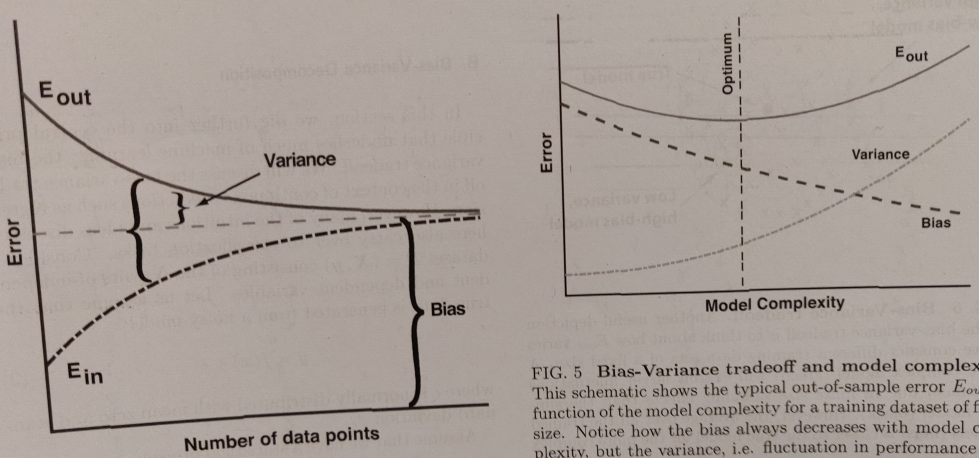
\includegraphics[width=0.7\linewidth]{gfx/InOutError.png}
	\caption{}
	\label{fig:errorbehaviour}
\end{figure}
Compare the behaviour of both errors with increasing number of data points, left graph of \ref{fig:errorbehaviour}, and the out-of-sample error with increasing model complexity, right graph of \ref{fig:errorbehaviour}. As for the left graph, we can look at the difference between the generalization ($E_{out}$) and training error ($E_{in}$), i.e. the big curly bracket representing $\abs{E_{in}-E_{out}}$. It measures how well our in-sample error reflects the out-of-sample error, and measures how much worse we would do on a new data set compared to our training data. For this reason, the difference between these errors is precisely the quantity that measures the difference between fitting and predicting. \emph{Models with a large difference between the in-sample and out-of-sample errors are said to \textbf{overfit} the data}. 
\begin{mybox}{}
	One of the lessons of statistical learning theory is that it is not enough to simply minimize the training error, because the out-of-sample error can still be large.
\end{mybox}
Considering the right graph, model  complexity is, in many cases, related to the number of parameters we are using to approximate the true function $f(x)$. If we consider a training dataset of a fixed size, $E_{out}$ will be a non-monotonic function of the model complexity, and is generally minimized for models with \emph{intermediate} complexity. The underlying reason for this is that, even though using a more complicated model always reduces the bias, at some point the model becomes too complex for the amount of training data and the generalization error becomes large due to high variance.
\begin{mybox}{}
Thus, to minimize $E_{out}$ and maximize our predictive power, it may be more suitable to use a more biased model with small variance than a less-biased model with large variance. This is is, again, the \emph{bias-variance} tradeoff we introduced above.
\end{mybox} 
Another way to understand this tradeoff is the following. Due to sampling noise from having finite size data sets, the learned models will differ for each choice of training sets. In general, more complex models need a larger amount of training data. For this reason, the fluctuations in the learned models (variance) will be much larger for the more complex model than the simpler model. However, if we consider the asymptotic performance as we increase the size of the training set (the bias), it is clear that the complex model will eventually perform better than the simpler model. Thus, depending on the amount of training data, it may \textbf{be more favourable to use a less complex, high-bias model to make predictions}.
























\section{Statistics}
Statistical modelling revolves around estimation or prediction.
\subsection{Difference between estimation and prediction}
Note first and foremost that techniques in ML tend to be more focused on prediction rather than estimation, which means that we will mostly treat prediction problems in this compendium. This is for example because an artificially intelligent agent needs to be able to recognize objects in its surroundings and predict the behaviour of its environment in order to make informed choices.\\
\subsubsection{Contrasting the two}
Estimation and prediction problems can be cast into a common conceptual framework. In both cases, we choose some observable quantity $\mx$ of the system we are studying (e.g. an interference pattern) that is related to some parameters $\mt$ (e.g. the speed of light) of a model $p(\mx|\mt)$ that describes the probability of observing $\mx$ given $\mt$.\\
Now we perform an experiment to obtain a dataset $\mX$ and use these data to fit the model. Typically,  ’fitting’ the model involves finding $\hat{\mt}$ that provides the best explanation for the data. In the case when ’fitting’ refers to the method of least squares, the estimated parameters maximize the probability of observing the data (i.e., $\hat{\mt}=\arg \max_{\mt}\{p(\mX|\mt) \}$).\\
\begin{mybox}{Estimation vs Prediction}
	\emph{Estimation problems} are concerned with the accuracy of $\hat{\mt}$, whereas \emph{prediction problems} are concerned with the ability of the model to predict new observations (i.e., the accuracy of $p(\mx|\hat{\mt})$. Although the goals of estimation and prediction are related, they often lead to different approaches.
\end{mybox}


\subsection{Mathematical motivation to presented key ideas}
We begin with an unknown function
$y = f (x)$ and fix a \emph{hypothesis set} $\mH$ consisting of all functions we are willing to consider, defined also on the domain of $f$ . This set may be uncountably infinite (e.g. if
there are real-valued parameters to fit). The choice of
which functions to include in $\mH$ usually depends on our
intuition about the problem of interest. The function
$f (x)$ produces a set of pairs $(x_i , y_i ), i = 1 . . . N$ , which
serve as the observable data. Our goal is to select a function from the hypothesis set $h \in \mH$ that approximates
$f (x)$ as best as possible, namely, we would like to find
$h \in \mH$ such that $h \approx f$ in some strict mathematical
sense which we specify below. 
\begin{mybox}{}
If this is possible, we say
that we \emph{learned} $f (x)$. 
\end{mybox}
But if the function $f (x)$ can, in
principle, take any value on \emph{unobserved inputs}, how is it
possible to learn in any meaningful sense ?\\
The answer is that learning is possible in the restricted
sense that the fitted model will probably perform approximately as well on new data as it did on the training data.
How can we evaluate the performance of our model then ?\\
As discussed in \ref{subsec:performanceeval}, once an appropriate error function $E$ is chosen for the
problem under consideration (e.g. sum of squared errors
in linear regression), we can define the in-and out-of-sample error to then minimize the out-of-sample error, with the variance-bias tradeoff in mind, to achieve robust predictions.
\subsubsection{Bias-Variance Decomposition for one Classifier}
\label{subsubsec:biasvarianceMathematicaloneClassifier}
Here we give a mathematical motivation to the bias-variance tradeoff discussed in \ref{subsubsec:biasvariancetradeoff}.\\
Consider a
dataset $\mD = (\mx, \mathbf{y})$ consisting of the $N$ pairs of independent and dependent variables. Let us assume that the
true data is generated from a noisy model
\be 
y = f (x) + \epsilon
\ee 
where $\epsilon$ is normally distributed with mean zero and standard deviation $\sigma_\epsilon$, i.e. the ’noise’.
Assume that we have a statistical procedure (e.g. least-
squares regression) for forming a predictor $f (\mx; \hat{\mathbf{θ}})$ that
gives the prediction of our model for a new data point $\mx$.
This estimator is chosen by minimizing a cost function
which we take to be the squared error
\be 
\label{eq:statCostFct}
\mC(\mathbf{y}, f(\mx; \mathbf{θ})) = \sum_i (y_i - f(x_i; \mathbf{θ}))^2.
\ee 
Therefore, the estimates for the parameters
\be 
\hat{\mathbf{θ}} =\arg \min_{θ} \mC(\mathbf{y}, f(\mx;\mathbf{θ}) )
\ee 
are a function of the dataset, $\mD$. We would obtain a
different error $\mC( \mathbf{y}_j , f (\mx_j ; \hat{\mathbf{θ}}_{\mD_j}))$ for each dataset $\mD_j =
(\mathbf{y}_j , \mx_j )$ in a universe of possible datasets obtained by
drawing $N$ samples from the true data distribution. We
denote an expectation value over all of these datasets as
$\mathbb{E}_{\mD}$.


\begin{mybox}{Errors}
	Combining these expressions,
	we see that the expected \emph{out-of-sample error}
	\be 
	 E_{out} := \mathbb{E}_{\mD,\epsilon}[\mC(\mathbf{y}, f (\mx; \hat{\mathbf{θ}}_{\mD} ))],
	\ee 
	 can be decomposed as
	 \be 
	E_{out} = \text{Bias}^2 + \text{Var} + \text{Noise},
	\ee
	with
	\begin{align*}
	\text{Noise}&=\sum_i \sigma^2_\epsilon,\; \text{Var}=\sum_i \mathbb{E}_{\mD}[(f (\mx_i ; \hat{\mathbf{θ}}_{\mD} ) − \mathbb{E}_{\mD}[f (\mx_i ; \hat{\mathbf{{θ}}}_{\mD})])^2 ],\\
	\text{Bias}^2&=\sum_i (f (\mx_i ) − \mathbb{E}_{\mD}[f ((\mx_i ;\hat{(\mathbf{θ}}_{\mD} )])^2.
	\end{align*}
	The variance measures how much our estimator fluctuates due
	to finite-sample effects and the bias measures the deviation of the expectation value of
	our estimator (i.e. the asymptotic value of our estimator
	in the infinite data limit) from the true value.
\end{mybox}
This gives us a mathematical tradeoff of the concepts discussed in \ref{subsec:performanceeval} and in particular in \ref{fig:errorbehaviour}.
\begin{mybox}{Bias-variance trade-off}
	The bias-variance tradeoff summarizes the fundamental tension in machine learning, particularly supervised
	learning, between the complexity of a model and the
	amount of training data needed to train it. Since data
	is often limited, in practice it is often useful to use a
	less-complex model with higher bias – a model whose
	asymptotic performance is worse than another model –
	because it is easier to train and less sensitive to sampling
	noise arising from having a finite-sized training dataset
	(smaller variance).
\end{mybox}
\subsubsection{Bias-Variance Decomposition for Ensembles}
\label{subsubsec:biasvarianceMathematicalEnsemble}
We will discuss the bias-variance tradeoff in the context of continuous predictions such as regression \ref{sec:linearRegression}. However, many of the intuitions and ideas discussed here also carry over to classification tasks, cf. \ref{sec:logisticRegression}. Consider a data set consisting of data $\mX_{\mL}=\{(y_j,\mx_j),j=1\dots n \}$ as above. Assume that we have a statistical procedure (e.g. OLS \ref{eq:lregOLS})) for forming a predictor $\hat{g}_{\mL}(\mx)$ that gives the prediction of our model for a new data point $\mx$ given that we trained the model using a dataset $\mL$. We will now, however, consider an ensemble of estimators $\{\hat{g}_{\mL}(\mx_i)\}$. Given a dataset $\mX_{\mL}$ and hyper-parameters $\mt$ that parametrize members of our ensemble, we will consider a procedure that deterministically generates a model $\hat{g}_{\mL}(\mx_i,\mt)$ given $\mX_{\mL}$ and $\mt$. We assume that the $\mt$ includes some random parameters that introduce stochasticity into our ensemble (e.g. an initial condition for stochastic gradient descent or a random subset of features or data points used for training.) Concretely, with a given dataset $\mL$ one has a learning algorithm $\mA$ that generates a model $\mA(\mt,\mL)$ based on a deterministic procedure which introduced stochasticity through $\mt$ in its execution on dataset $\mL$. \\
We will be concerned with the expected prediction error of the \emph{aggregate ensemble predictor}
\be 
\label{eq:biasvarianceAggregateEnsemblePredictor}
\hat{g}^A_{\mL}(\mx_i,\{\mt\} ) = \frac{1}{M} \sum_{n=1}^M \hat{g}_{\mL}(\mx_i,\mt_m).
\ee 
For future reference, let us define the mean, variance and covariance (i.e. the connected correlation function in the language of physics), and the normalized correlation coefficient of a single randomized model $\hat{g}_{\mL}(\mx,\mt_m)$ as 
\begin{align}
	\label{eq:biasvarianceDefinitionsMoments}
	\mathbb{E}_{\mL,\mt_m}[\hat{g}_{\mL}(\mx,\mt_m)] &= \mu_{\mL,\mt_m}(\mx) \nonumber \\
	\mathbb{E}_{\mL,\mt_m}[\hat{g}_{\mL}(\mx,\mt_m)^2]- \mathbb{E}_{\mL,\mt_m}[\hat{g}_{\mL}(\mx,\mt)]^2 &= \sigma^2_{\mL,\mt_m}(\mx) \nonumber \\
	\mathbb{E}_{\mL,\mt_m}[\hat{g}_{\mL}(\mx,\mt_m) \hat{g}_{\mL}(\mx,\mt_{m^\prime})] -\mathbb{E}_{\mt}[\hat{g}_{\mL}(\mx,\mt_m) ]^2 &= C_{\mL,\mt_m,\mt_{m^\prime}} (\mx) \nonumber \\
	\rho(\mx) &= \frac{C_{\mL,\mt_m,\mt_{m^\prime}}(\mx) }{\sigma^2_{\mL,\mt}}.
\end{align}
Note that the expectation $\mathbb{E}_{\mL,\mt_m}[\cdot]$ is computed over the joint distribution of $\mL$ and $\mt_m$. Also by definition, we assume $m\neq m^\prime$.\\
Now, we can, as in \ref{subsubsec:biasvarianceMathematicaloneClassifier}, define the expected generalization (out-of-sample) error for the ensemble 
\begin{align}
\label{eq:biasvarianceGeneralizationErrorEnsemble}
\mathbb{E}_{\mL,\mt_m}[C(\mX,\hat{g}^A_{\mL}(\mx))] &= \mathbb{E}_{\mL,\epsilon,\mt} \left[ \sum_i (\my_i - \hat{g}^A_{\mL} (\mx_i,\{\mt\} ))^2\right]\nonumber \\
&= Bias^2(\mx_i) + Var(\mx_i)+ \sum_i \sigma^2_{\epsilon_i},
\end{align}
where one defines the bias of an aggregate predictor 
\be 
\label{eq:biasvarianceBiasEnesemble}
Bias^2(\mx) \equiv \left(f(\mx) - \mathbb{E}_{\mL,\mt}[\hat{g}^A_{\mL} (\mx,\{\mt\}) ]\right)^2
\ee 
and the variance as
\bse 
Var(\mx) = \mathbb{E}_{\mL,\mt}\left[ (\hat{g}^A_{\mL}(\mx,\{\mt\}) - \mathbb{E}_{\mL,\mt}[\hat{g}^A_{\mL}(\mx,\{\mt\})])^2 \right]. 
\ese 
So far the calculation for ensembles is almost identical to that of a single estimator, compare \ref{subsubsec:biasvarianceMathematicaloneClassifier}.
\begin{mybox}{Crux of Bias-Variance for Ensembles}
	However, since the aggregate estimator is a sum of estimators, its variance implicitly depends on the correlations between the individual estimators in the ensemble. One finds
	\be 
	\label{eq:biasvarianceVarianceEnsembleCrux}
	Var(\mx) = \rho(\mx) \sigma^2_{\mL,\mt} + \frac{1-\rho(\mx)}{M} \sigma^2_{\mL,\mt}.
	\ee 
	This \ref{eq:biasvarianceVarianceEnsembleCrux} is the key to understanding the power of random ensembles. Notice that by using large ensembles ($M\rightarrow \infty$), we can significantly reduce the variance, and for completely random ensembles where the models are uncorrelated ($\rho(\mx)=0$), maximally suppresses the variance !\\
	Thus, reducing the aggregate predictor beats down fluctuations due to finite-sample effects. They key, as \ref{eq:biasvarianceVarianceEnsembleCrux} indicates, is to \textbf{decorrelate the models as much as possible while still using a very large ensemble.}
\end{mybox}
\begin{mybox}{What does this do to the bias ?}
One can be worried that this comes at the expense of a very large bias. This turns out not to be the case. When models in the ensemble are completely random, the bias of the aggregate predictor is just the expected bias of a single model 
\bse 
Bias^2(\mx) = (f(\mx) - \mu_{\mL,\mt})^2.
\ese 
\textbf{Thus, for a random ensemble one can always add more models without increasing the bias.}
\end{mybox}

Therefore, the correlation between models that constitute the ensemble is the key property here. It is important for two reasons. First, holding the ensemble size fixed, averaging the predictions of correlated models reduces the variance less than averaging uncorrelated models. Second, in some cases, correlations between models within an ensemble can result in an \emph{increase} in bias, offsetting any potential reduction in variance gained from ensemble averaging.\\
This will be discussed in the context of bagging  \ref{subsubsec:ensemblesBagging}.










\subsection{Mathematical set-up of every problem ever}
As described quantitatively in \ref{subsec:recipeML}, every problem in ML can be designed via a recipe which is presented now qualitatively.\\
\subsubsection{Set-up of the notation}
Suppose we are given a dataset with $n$ samples $\mD = \{(y_i,\mx^{(i)} )\}^n_{i=1}$, where $\mx^{(i)}$ is the $i$-th observation vector while $y_i$ is its corresponding (scalar) response. We assume that every sample has $p$ \emph{features}, namely,
\bse 
\mx^{(i)} \in \mR^p.
\ese  
Let $f$ be the true function/model that generated these samples via
\bse 
y_i  = f(\mx^{(i)}, \mw_{true}) + \epsilon_i,
\ese 
where $\mw_{true}\in \mR^p$ is a \emph{parameter} vector and $\epsilon_i$ is some i.i.d. white noise with zero mean and finite variance. Conventionally, we cast all samples in an $n\times p$ matrix, the \emph{design matrix}
\bse 
\mX \in \mR^{n\times p}
\ese 
with the rows 
\bse 
\mX_{i,:} = \mx^{(i)} \in \mR^p,\quad i =1,\dots,n
\ese 
being \emph{observations} and the columns
\bse 
\mX_{:,j} \in \mR^n,\quad j=1,\dots,p 
\ese 
being measured \emph{features}(i.e. feature predictors).\\
Bear in mind that this function $f$ is never known to us explicitly, though in practice we usually presume its functional form.
\begin{example}
	For example, in \emph{linear regression}, we assume
	\bse 
	y_i = f(\mx^{(i)};\mw_{true}) + \epsilon_i= \mw^T_{true} \mx^{(i)} + \epsilon_i
	\ese 
	for some unknown but fixed $\mw_{true}\in \mR^p$.
\end{example}










\subsubsection{Set-up of the problem}
We want to find a function $g$ with parameters $\mw$ fit to the data $\mD$ that can best approximate $f$. This is done when we have found a $\hat{\mw}$ such that $g(\mx;\hat{\mw})$ yields our best estimate of $f$. Now we can use this $g$ to make predictions about the response $y_0$ for a new data point $\mx_0$.\\
Therefore:\\
Fitting a given set of samples $(y_i,\mx_i)$ means relating the independent variables $\mx_i$ to their responses $y_i$. The next step is to assume some \emph{models} that might explain the measurements and measuring their performance, i.e. finding the function $g$ such that
\bse 
y_i = g(\mx_i;\mw).
\ese 
We call $g(\mx^{(i)},\mw)$ the \emph{predictor}. Recall that the optimal choice of predictor depends on, among many other things, the functions used to fit the data and the underlying noise level.
We then try to minimize the errors made in explaing the given set of measurements based on our model $g$ by tuning the parameters $\mw$. To do so, we need to first define the error function (formally called the  \emph{loss function}) that characterizes the deviation of our prediction from the actual response




\subsubsection{On statistical language}
As described above, a ML or statistics problem is defined via a optimization (minimization) problem of an error function, the solution to this is given by some estimator
\be 
\hat{\mw}_{Problem} = \arg \min_{\mw \in \mR^p} \mC(\mX, g(\mw,\my)).
\ee 
The bias (or bias function) of an estimator is the difference between this estimator's expected value and the true value of the parameter being estimated.


\subsection{Language of optimization problems}
\subsubsection{Convexity}
Recall that a set $C\subset\mR^n$ is called \emph{convex} if any  $x,y\in C$  and  $t\in [0,1]$,
\bse 
tx + (1-t) y \in C.
\ese 

In other words, every line segments joining  $x,y$  lies entirely in  $C$ .

A function $f:\mR^n \rightarrow \mR$ is called \emph{convex} if its domain $\text{dom}(f)$  is a convex set and for any  $x,y\in \text{dom}(f)$  and $ t\in[0,1]$ ,
\bse 
f(tx+(1-t)y) \leq t f(x) + (1-t) f(y).
\ese 

In other words, the function lies below the line segment joining $ f(x)$  and $ f(y)$ . This function  $f$  is called \emph{strictly convex} if this inequality holds strictly for  $x \neq y$  and  $t \in (0,1)$ .
\begin{mybox}{}
Why is convexity important? \\
\textbf{For convex functions, any local minimizer is a global minimizer}. Algorithmically, this means that in the minimization (optimization) procedure, as long as we're "going down the hill" and agree to stop when we can't go any further, then we've hit the global minimum. In addition to this, there's a menagerie of beautiful theory regarding convex duality and optimality, which gives us a way of understanding the solutions even before solving the problem itself.
\end{mybox}


\section{Overview of Bayesian Inference}
\label{sec:bayes}
Bayesian inference provides a set of principles and procedures for learning from data and for describing uncertainty.
\subsection{Language}
\begin{mybox}{Likelihood function}
	The \emph{likelihood function} 
	\be
	\label{eq:bayesLikelihoodFct}
	p(\mX|\mt)
	\ee 
	describes the probability of observing a dataset $\mX$ for a given value of the unknown parameters $\mt$. It is a function of the parameters $\mt$ with the data $\mX$ held fixed. Furthermore, it is determined by the model and the measurement noise.
\end{mybox}
\begin{mybox}{Prior distribution}
	The \emph{prior distribution} $p(\mt)$ describes any knowledge that we have about the parameters before we collect the data.
\end{mybox}
\begin{mybox}{Priors}
	\label{subsec:priors}
	There are two general classes of priors: 
	\begin{enumerate}
		\item The \emph{uninformative prior}:\\
		We choose this one if we do not have any specialized knowledge about $\mt$ before we look at the data. 
		\item The \emph{informative prior}:\\
		If we have prior knowledge, we choose an informative prior that accurately reflects the knowledge that we have about $\mt$. This one is commonly employed in ML:
	\end{enumerate}
	There is another not so important prior, the \emph{hierarchical prior}. This describes the process of choosing a hyperparameter by defining a prior distribution for it (via an uninformative prior) and then averaging the posterior distribution over all choices of the hyperparameter.
\end{mybox}
Using an informative prior tends to decrease the variance of the posterior distribution while, potentially, increasing its bias. It is beneficial if the decrease in variance is larger than the increase in bias. In high-dimensional problems, it is reasonable to assume that many of the parameters will not be strongly relevant. Therefore, many of the parameters of the model will be zero or close to zero. We can express this belief using two commonly used priors.
\begin{mybox}{Two informative priors commonly employed}
	The \emph{Gaussian prior} is used to express the assumption that many of the parameters will be small 
	\be 
	\label{eq:bayesGaussianprior}
	p(\mt|\lambda) = \prod_j \sqrt{\frac{\lambda}{2 \pi}} e^{- \lambda \theta^2_j},
	\ee
	where $\lambda$ is a \emph{hyperparameter}. The \emph{Laplace prior} is used to express the assumption that many of the parameters will be zero
	\be 
	\label{eq:bayesLaplacianprior}
	p(\mt|\lambda) = \prod_j \frac{\lambda}{2} e^{-\lambda \abs{\theta_j}}.
	\ee 
	The hyperparameter can either be chosen via a hierarchical prior employing MCMC or  by simply finding a good value of $\lambda$ using an optimization procedure (see linear regression).
\end{mybox}
Indeed, a Gaussian prior is the \emph{conjugate prior} that gives a Gaussian posterior. For a given likelihood, conjugacy guarantees the preservation of prior distribution at the posterior level.
\begin{example}
	For example, for a Gaussian (Geometric) likelihood with a Gaussian (Beta) prior, the posterior distribution is still a Gaussian (Beta) distribution.
\end{example}
\begin{mybox}{hyperparameters}
	A \emph{hyperparameter} or \emph{nuisance variable} is a parameter whose value is set before the learning process begins. By contrast, the values of other \emph{parameters} are derived via training.
\end{mybox}

\subsubsection{Connecting statistics and bayesian framework}
To connect a statistical model to the Bayesian framework, we often write the model as
\be 
\label{eq:bayesianFreqConnectionModel}
p(y|\mx,\mt) = \mathcal{N}(y|\mu(\mx),\sigma^2(\mx)).
\ee 
In other words, our model is defined by a conditional probability that depends not only on data $\mx$ but on some model parameters $\mt$.
\begin{example}
	For example, if the mean is a linear function of $\mx$ given by $\mu = \mx^T \mw$, and the variance is fixed $\sigma^2(\mx) = \sigma^2$, then $\mt=(\mw,\sigma^2)$.
\end{example}











\subsection{Calculations}
\begin{mybox}{Bayes' rule}
	The \emph{posterior distribution} $p(\mt|\mX)$ describes our knowledge about the unknown parameter $\mt$ after observing the data $\mX$. It is given via Bayes' rule
	\be 
	\label{eq:bayesrule}
	p(\mt | \mX) = \frac{p(\mX|\mt) p(\mt) }{\int \md \mt^\prime p(\mX | \mt^\prime) p(\mt^\prime)}.
	\ee
\end{mybox}
The denominator is difficult in practice such that one normally uses Markov Chain Monte Carlo (MCMC) to draw random samples from $p(\mt|\mX)$.
\subsection{Estimation}
\subsubsection{Maximum Likelihood estimation}
\label{subsubsec:bayesEstMLE}
In statistics, many problems rely on estimation of some parameters of interest.
\begin{example}
	For example, suppose we are given the height data of $20$ junior students from a regional high school, but what we are interested in is the average height of all high school juniors in the whole country. It is conceivable that the data we are given are not representative of the student population as a whole.
\end{example}
It is therefore necessary to devise a systematic way to perform reliable estimation. Here we present the \emph{maximum likelihood estimation} (MLE), and show that MLE for $\mt$ is the one that minimizes the mean squared error (MSE) used in \ref{eq:lregOLS}.
\begin{mybox}{MLE}
	Many common statistical procedures such as least-square fitting can be cast as MLE. In MLE, one chooses the parameters $\hat{\mt}$ that maximizes the likelihood (or equivalently the log-likelihood since log is a monotonic function) of the observed data $\mX$ (or equivalently $\mD$):
	\be 
	\label{eq:bayesMLE}
	\hat{\mt}= \arg \max_{\mt} \log p(\mX |\mt).
	\ee 
	In MLE we therefore choose the parameters that maximize the probability of seeing the observed data given our generative model.
\end{mybox}
Using the assumption that samples are i.i.d., we can write the \emph{log-likelihood} as 
\be 
\label{eq:bayesLogLikelihood}
l(\mt) \equiv \log p(\mD|\mt) = \sum_{i=1}^n \log p(y_i|\mx^{(i)},\mt).
\ee 
Note that the conditional dependence of the response variable $y_i$ on the independent variable $\mx^{(i)}$ in the likelihood function is made explicit since, in most applications, the observed value of data, $y_i$, is predicted based on $\mx^{(i)}$ using a model that is assumed to be a probability distribution that depends on unknown parameters $\mt$. This distribution, when endowed with $\mt$, can, as we hope, potentially explain our prediction on $y_i$. By definition, such distribution is the likelihood function \ref{eq:bayesLikelihoodFct}. We stress that this notation does \emph{not} imply $\mx^{(i)}$ is unknown, it is still part of the observed data!
\begin{mybox}{Error function}
The negative of the log-likelihood gives us the error function
\be 
\label{eq:bayesErrorFct}
E(\mt)=-l(\mt).
\ee 
\end{mybox}
\subsubsection{Maximum-a-Posteriori estimation}
\ref{eq:bayesMLE} provides the tools for computing the posterior distribution $p(\mt|\mX)$, which uses probability as a framework for expressing our knowledge about the parameters $\mt$. In most cases, however, we need to summarize our knowledge and pick a single ’best’ value for the parameters. In principle, the specific value of the parameters should be chosen to maximize a utility function. In practice, however, we usually use on of two choices:
\begin{enumerate}
	\item The posterior mean, or  \emph{Bayes estimate}
	\be 
	\label{eq:bayesBayesEstimate}
	\expval{\mt} = \int \md \mt \mt \;p(\mt |\mX),
	\ee 
	or
	\item the posterior mode, also called the \emph{maximum-a-posteriori} (MAP) estimate
	\be 
	\label{eq:bayesMAPestimate}
	\hat{\mt}_{MAP} = \arg \max_{\mt} p(\mt |\mX).
	\ee 
	This estimate gives the parameters at which the posterior probability distribution is peaked
\end{enumerate}
While the Bayes estimate minimizes the mean-squared error, MAP estimate is often used instead because it is easier to compute.
\subsubsection{Out-of-Bag estimators}
\label{subsubsec:bayesOOBestimators}
For ensemble methods, especially random forest \ref{subsec:ensemblesRandomForest}, there exists another object for estimation, the \emph{out-of-bag (OOB) estimates}.
This is discussed in more detail in \ref{subsec:ensemblesRandomForest}.
\subsection{Bayesian view on regularization}
As discussed in \ref{subsec:performanceeval}, \emph{we can't make predictions without making assumptions}. Thus, it is sensible to introduce priors that reflect the fact that we are likely to be undersampled (especially in high dimensions).\\
We can supplement an error function with a regularizer that prevents overfitting. From a Bayesian point of view, the regularization can be thought of as a prior on parameters. Minimizing the combined in-sample error $+$ regularization terms is the same as the \emph{Maximum a posteriori probability} (MAP) estimate in Bayesian regression \ref{eq:bayesMAPestimate}. Note that in a true Bayesian approach, we should not use the mode of the posterior but the average over all possible choices of parameters weighted by their posterior probability. In practice, this is often not done (for computational and practical reasons).
\subsubsection{MAP estimator in the context of regularization}
Instead of maximizing the the log-likelihood \ref{eq:bayesLogLikelihood} to obtain a good estimator \ref{eq:bayesMLE},  let us maximize the log posterior $\log p(\mt|\mD)$, which we can get via Bayes' rule \ref{eq:bayesrule}. Then, the MAP estimator becomes 
\be 
\hat{\mt}_{MAP} \equiv \arg \max_{\mt} \log p(\mD|\mt) + \log p(\mt).
\ee 
A common choice for the prior $p(\mt)$ is the Gaussian distribution. Consider the Gaussian prior \ref{eq:bayesGaussianprior} with zero mean and variance $\tau^2$, namely
\bse 
p(\mw) =\prod_j \mathcal{N}(w_j|0,\tau^2).
\ese 
Then, we can recast the MAP estimator into
\begin{align}
	\label{eq:bayesMAPestimatorGaussianPrior}
	\hat{\mt}_{MAP} &= \arg \max_{\mt} \left[ -\frac{1}{2 \sigma^2} \sum_{i=1}^n (y_i-\mw^T \mx^{(i)} )^2 - \frac{1}{2 \tau^2 } \sum_{j=1}^n w^2_j\right]\nonumber \\
	&= \arg \max_{\mt} \left[- \frac{1}{2 \sigma^2} \norm{\mX \mw -\my }^2_2 - \frac{1}{2\tau^2} \norm{\mw}^2_2\right].
\end{align}
This is used later on to cast linear regression into bayesian language, \ref{subsec:lregBayesian}.






\section{Mathematical tools}
\label{sec:math}
\subsection{Sampling methods}

\subsubsection{Empirical Bootstrapping}
\label{subsubsec:ensemblesBootstrapping}
Empirical bootstrapping is a method to enlarge a sparse dataset, we use it in bagging, cf. \ref{subsubsec:ensemblesBagging}.\\
Suppose we are given a finite set of $n$ data points $\mD=\{X_1,\dots,X_n\}$ as training samples and our job is to construct measures of confidence for our sample estimates (e.g. the confidence interval or mean-squared error of sample median estimator). To do so, one first samples $n$ points \textbf{with replacement} from $\mD$ to get a new set $\mD^{*(1)}=\{X^{*(1)}_1,\dots,X^{*(1)}_n\}$. called a \textbf{bootstrap sample}, which possibly contains repetitive elements. Then we repeat the same procedure to get in total $B$ such sets: 
\bse 
\mD^{*(1)},\dots, \mD^{*(B)}.
\ese 
The next step is to use these $B$ bootstrap sets to get the \textbf{bootstrap estimate} of the quantity of interest. For example, let $M^{*(k)}_n=$Median$(\mD^{*(k)})$ be the sample median of bootstrap data $\mD^{*(k)}$. Then we can construct the variance of the distribution of bootstrap medians as
\be 
\label{eq:ensemblesBootrapingVariance}
\hat{Var}_B(M_n)=\frac{1}{B-1} \sum_{k=1}^B \left[M^{*(k)}_n-\bar{M}^{*}_n\right]^2 = \sigma^2 \stackrel{n\rightarrow \infty}{\longrightarrow} \frac{1}{n}
\ee 
where 
\bse 
\bar{M}^{*}_n=\frac{1}{B} \sum_{k=1}^{B} M^{*(k)}_n
\ese 
is the mean of the median of all bootstrap samples.
\\
For $n\rightarrow\infty$, it was shown that the distribution of the bootstrap estimate will be a Gaussian centred around $\hat{M}_n(\mD)=$Median$(X_1,\dots,X_n)$ with standard deviation proportional to $1/\sqrt{n}$. This mean that the bootstrap distribution $\hat{M}^*_n-\hat{M}_n$ approximates fairly well the sampling distribution $\hat{M}_n-M$ from which we obtain the training data $\mD$. Note that $m$ is the median based on which the true distribution $\mD$ is generated. In other words, if we plot the histogram of $\{M^{*(k)}_n \}^B_{k=1}$, we will see that in the large $n$ limit it can be well fitted by a Gaussian which sharp peaks at $\hat{M}_n(\mD)$ and vanishing variance whose definition is given by \ref{eq:ensemblesBootrapingVariance}.

\begin{figure}[h!]
	\centering
	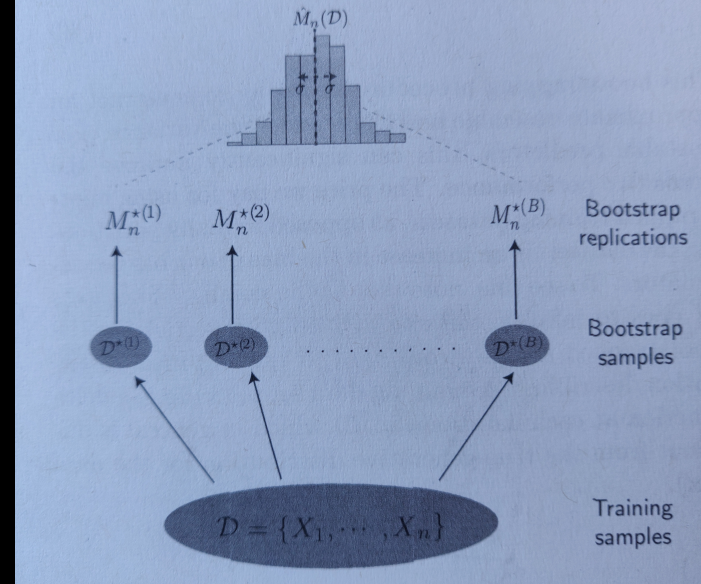
\includegraphics[width=0.7\linewidth]{gfx/Bootstrapping}
	\caption{}
	\label{fig:bootstrapping}
\end{figure}
Figure \ref{fig:bootstrapping} shows the procedure of empirical bootstrapping. 
\begin{mybox}{Bootstrapping - Summary}
	The goal is to assess the accuracy of a statistical quantity of interest, which in the main text is illustrated as the sample median $\hat{M}_m(\mD)$. We start from a given dataset $\mD$ and bootstrap $B$ size $n$ datasets $\mD^{*(1)},\dots,\mD^{*(B)}$ called the bootstrap samples. Then we compute the statistical quantity of interest on these bootstrap samples to get the median $M^{*(k)}_n$, for $k=1,\dots,B$. These are then used to evaluate the accuracy of $\hat{M}_n(\mD)$. It can be shown that in the $n\rightarrow\infty$ limit the distribution of $M^{*(k)}_n$ would be a Gaussian centred around $\hat{M}_n(\mD)$ with variance $\sigma^2$ defined by \ref{eq:ensemblesBootrapingVariance}.
\end{mybox}


\subsection{Algorithms}
\subsubsection{Decision Trees}
\label{subsubsec:ensemblesRFDecisionTree}
Decision trees are high-variance, weak classifiers that can be easily randomized, and as such, are ideally suited for ensemble-based methods.
They are employed for random forests, cf. \ref{subsec:ensemblesRandomForest}.\\
A decision tree uses a series of questions to hierarchically partition the the data. Each branch of the decision tree consists of a question that splits the data into smaller subsets with the leaves (end points) of the tree corresponding to the ultimate partitions of the data. When using decision trees for classification, the goal is to construct trees such that the partitions are informative about the class label. It is clear that more complex decision trees lead to finer partitions that give improved performance on the training set. However, this \textbf{generally leads to over-fitting}, limiting the out-of-sample performance. For this reason, in practice almost all decision trees use some form of regularization (e.g. maximum depth for the tree) to control complexity and reduce overfitting. Decision trees also have extremely high variance, and are often extremely sensitive to many details of the training data. This is not surprising since decision trees are learned by partitioning the training data. Therefore, \textbf{individual decision trees are weak classifiers.}\\
\\
However, these same properties make them ideal for incorporation in an ensemble method.\\




























\section{Gradient descent}
\label{sec:gd}
\subsection{Simple gradient descent}

As always in the context of ML, we want to minimize the cost function $E(\mathbf{θ})=\mC(\mx,g(\mathbf{θ}))$.
\begin{mybox}{Gradient descent}
The simplest gradient descent (GD) algorithm is characterized by the following \emph{update rule} for the parameters $\mathbf{θ}$. Initialize the parameters to some value $\mathbf{θ}_0$ and iteratively update the parameters according to the equation
\be
\centering\label{eq:gdsimple}
\mathbf{v}_t = \eta_t \nabla_{θ} E(\mathbf{θ}_t),\quad \mathbf{θ}_{t+1} = \mathbf{θ}_t-\mathbf{v}_t
\ee 
where we have introduced the \emph{learning rate} $\eta_t$ (one hyperparameter of the model), that controls how big a step we should take in the direction of the gradient at time step $t$.
\end{mybox}
For sufficiently small choice of $\eta_t$, this method will converge to a \emph{local minimum} of the cost function, however this is computationally expensive. In practice, one usually specifies a ’schedule’ that decreases $\eta_t$ at long times (common schedules include power law and exponential decay in time).\footnote{Note that  Newton's method is a first-order approximation of GD method, which is not practical as it is a computationally expensive algorithm. However, Newton's method automatically adjusts the step size so that one takes larger steps in flat directions with small curvature and smaller steps in steep directions with large curavture. This gives an intuition of how to modify GD methods to get better results.}
The simple GD has the following limitations
\begin{enumerate}
\item GD finds local minima of the cost function.\\
Because in ML we are often dealing with extremely rugged landscapes with many local minima, this can lead to poor performance.
\item Gradients are computationally expensive to calculate for large datasets.
\item GD is very sensitive to choices of the learning rates.\\
Ideally, we would ’adaptively’ choose the learning rates to match the landscape.
\item GD treats all directions in parameter space uniformly.
\item GD is sensitive to initial conditions.
\item GD can take exponential time to escape saddle points, even with random initialization..
\end{enumerate}
These limitiations lead to generalized GD methods which form the backbone of much of modern DL and NN.
\subsection{Modified gradient descent}
\subsubsection{Stochastic gradient descent (SGD) with mini-batches}
\label{subsubsec:gdSGD}
\begin{mybox}{SGD}
		In SGD, we replace the actual gradient over the full data at each gradient descent step by an approximation to the gradient computed using a minibatch. This introduces stochasticity and decreases the chance that our fitting algorithm gets stuck in isolated local minima, as you cycle over all minibatches one at a time.\\
The update rule is
	\be
	\centering\label{eq:gdstochastic}
	\mathbf{v}_t=\eta_t \nabla_{θ} E^{MB}(\mathbf{θ}),\quad \mathbf{θ}_{t+1} = \mathbf{θ}_t-\mathbf{v}_t.
	\ee 
\end{mybox}
\subsubsection{Algorithm gradient descent with momentum}
\marginpar{It has been argues that first-order methods (with appropriate initial conditions) can perform comparable to more expensive second-order methods, especially in the context of comples DL models.}
\begin{mybox}{GDM}
Introduce a ’momentum’ term into SGD which serves as a memory of the direction we are moving in parameter space. This helps the GD algorithm to gain speed in directions with persistent but small gradients even in the presence of stochasticity, while suppressing oscillations in high-curvature directions. The update rules is
\be 
\centering\label{eq:gdmomentum}
\mathbf{v}_t = \gamma \mathbf{v}_{t-1}+\eta_t \nabla_{θ} E^{MB}(\mathbf{θ}_t), \quad \mathbf{θ}_{t+1} = \mathbf{θ}_t-\mathbf{v}_t,
\ee
where we have introduced a momentum parameter $\gamma \in [0,1]$. 
\end{mybox}
\begin{mybox}{NAG}
	A final widely used variant of gradient descent with momentum is called the Nesterov accelerated gradient (NAG). In NAG, rather than calculating the gradient at the current position, one calculates the gradient at the position momentum will carry us to at time  $t+1$ , namely, $ θ_t−γ v_{t−1}$ . Thus, the update becomes
	\be 
	\centering\label{eq:gdNAG}
	\mathbf{v}_t = \gamma \mathbf{v}_t + \eta_t \nabla_{θ} E(\mathbf{θ}_t-\gamma \mathbf{v}_{t-1}),\quad \mathbf{θ}_{t+1} = \mt_{t}-\mathbf{v}_t.
	\ee 
\end{mybox}
\subsubsection{Methods that use the second moment of the gradient}
We would like to adaptively change the step size to match the landscape. This can be accomplished by tracking not only the gradient, but also the second moment of the gradient\footnote{Similar but avoiding the Hessian, which encodes local curvatures via second derivatives, as in Newton's method.}
\begin{mybox}{Root-mean-square propagation - RMSprop}
	In addition to keeping a running average of the first moment of the gradient, we also keep track of the second moment denoted by $\mathbf{s}_t=\mathbb{E}[\mathbf{g}^2_t]$. The update rule is 
	\be
	\centering\label{eq:gdRMSprop}
	\mathbf{g}_t=\nabla_{θ} E(\mathbf{θ}),\; \mathbf{s}_t=\beta \mathbf{s}_{t-1} + (1-\beta) \mathbf{g}^2_t,\; \mathbf{θ}_{t+1}=\mathbf{θ}_t - \eta_t \frac{\mathbf{g}_t}{\sqrt{\mathbf{s}_t+\epsilon}},
		\ee 
		where $\beta$ controls the averaging time of the second moment and is typically taken to be about $\beta=0.9$, $\eta_t$ is typically chosen to be $10^{-3}$, and $\epsilon\propto 10^{-8}$ is a small regularization constant to prevent divergencies. It is clear from this formula that the learning rate is reduced in directions where the gradient is consistently large.
\end{mybox}
\begin{mybox}{ADAM}
	In ADAM, we keep a running average of both the first and second moment of the gradient and use this information to adaptively change the learning rate for different parameters. In addition to keeping a running average of the second moments of the gradient (i.e $\mathbf{m}_t= \mathbb{E}[\mathbf{g}_t], \mathbf{s}_t=\mathbb{E}[\mathbf{g}^2_t]$), ADAM performs an additional bias correction to account for the fact that we are estimating the first two moments of the gradient using a running average (denoted by the hat in the update rule). The update rule is given by (where multiplication and division are once again understood to be element-wise operations)
	\begin{align}
		\centering\label{eq:gdADAM}
		\mathbf{g}_t &= \nabla_{θ} E(\mathbf{θ}), \quad \mathbf{m}_t =\beta_1 \mathbf{m}_{t-1} + (1-\beta_1) \mathbf{g}_t, \\
		\mathbf{s}_t &=\beta_2 \mathbf{s}_{t-1} + (1-\beta_2) \mathbf{g}^2_t,\quad \hat{\mathbf{m}}_t = \frac{\mathbf{m}}{1-(\beta_1)^t},\nonumber \\
		\hat{\mathbf{s}}_t &= \frac{\mathbf{s}_t}{1-(\beta_2)^t},\quad \mathbf{θ_{t+1}} = \mathbf{θ}_t - \eta_t \frac{\hat{\mathbf{m}}}{\sqrt{\hat{\mathbf{s}}_t} +\epsilon}\nonumber,
	\end{align}
where $\beta_1$ and $\beta_2$ set the memory lifetimes of the first and second moment (typically $\beta_{1,2} =\{0.9,0.99\}$ respectively, $\epsilon,\eta_t$ are same as in RMSprop).
\end{mybox}
The learning rates for RMSprop and ADAM can be set significantly higher than other methods due to their adaptive step sizes. For this reason, ADAM and RMSprop tend to be much quicker at navigating the landscape than simple momentum based methods.\footnote{Note that in some cases trajectories might not end up at the global minimum. This kind of landscape structure is generic in high-dimensional spaces where saddle points proliferate.}
\subsection{Practical tips for using GD}
Employ these tips for getting the best performance from GD based algorithms, especially in the context of deep neural networks (DNN)
\begin{enumerate}
	\item Randomize the data when making mini-batches.\\
	Otherwise, the GD method can fit spurious correlations resulting from the order in which data is presented.
	\item Transform your inputs.\\
	One simple trick for minimizing problems in difficult landscapes is to standardize the data by subtracting the mean and normalizing the variance of input variables. Whenever possible, also decorrelate the inputs. 
	\item Monitor the out-of-sample performance.\\
	Always monitor the performance of your model on a validation set (a small portion of the training data that is held out of the training process to serve as a proxy for the test set). If the validation error starts increasing then the model is beginning to overfit. Terminate the learning process. This \emph{early stopping} significantly improves performance in many settings.
	\item Adaptive optimization methods do not always have good generalization.\\
	Recent studies have shown that adaptive methods such as ADAM, RMSprop , and AdaGrad tend to have poor generalization to SGD or SGD with momentum, particularly in the high-dimensional limit (i.e. the number of parameters exceeds the number of data points). Although it is not clear at this state why sophisticated methods (e.g. ADAM, RMSprop, AdaGrad)  perform so well in training DNN such as generative adversarial networks (GANs), simpler procedures like properly-tuned plain SGD may work equally well or better in some applications.
\end{enumerate}







\section{Linear regression}
\label{sec:linearRegression}

\subsection{Least-square regressions -frequentist}
We'll consider ordinary least squares regression problem in which the "error function" is defined as the square from the deviation of our linear predictor to the true response. 
\begin{mybox}{OLS}
\emph{Ordinary least squares linear regression} (OLS) is defined as the minimization of the $L_2$ norm of the difference between the response $y_i$ and the predictor $g(\mx^{(i)};\mw)=\mw^T \mx^{(i)}$:
\be 
\centering\label{eq:lregOLS}
\min_{\mw \in \mR^p} \norm{\mX \mw -\my}^2_2 = \min_{\mw \in \mR^p}\sum_{i=1}^n (\mw^T \mx^{(i)} - y_i)^2.
\ee
Where \ref{eq:lregOLS} is the minimization of the loss function of OLS.\\
We are looking to find the parameters $\mw$ which minimize the $L_2$ error. Geometrically speaking, the predictor function $g$ defines a hyperplane in $\mR^p$. Minimizing the least squares error is therefore equivalent to minimizing the sum of all projections (i.e. residuals) for all points $\mx^{(i)}$ to this hyperplane. If $\rank (\mX)=p$ , namely, the feature predictors  $\mX_{:,1},\dots,\mX_{:,p}$  are linearly independent, then there exists unique solution to this problem, which we denote as $\hat{\mw}_{LS}$:
\be 
\centering\label{eq:lregOLSsolution}
\hat{\mw}_{LS} = \arg \min_{\mw \in \mR^p} \norm{\mX \mw - \my}^2_2 = (\mX^T \mX )^{-1} \mX^T \my,
\ee 
where we have assumed that $\mX^T\mX$ is inertible, which is often the case when $n\gg p$ (i.e. method works if number of data points exceeds number of features). The best fit of our data $\mX$ is
\be 
\label{eq:lregOLbestfit}
\hat{\my} = \mX \hat{\mw}_{LS} = \underbrace{\mX (\mX^T \mX)^{-1} \mX^T}_{\equiv P_{\mX}},
\ee 
where $P_{\mX}$ is the projection matrix which acts on $\my$ and projects it onto the column space of $\mX$, which is spanned by the predictors $\mX_{:,1},\dots,\mX_{:,p}$.
\end{mybox}
Note how we found the optimal solution $\hat{\mw}_{LS}$ in one shot, without doing any sort of iterative optimization.\\
What are the errors of OLS such that we can evaluate its performance according to \ref{subsec:performanceeval} ?\footnote{As we have seen, the difference between learning and fitting lies in the prediction on ’unseen’ data.}\\
We find that the average \emph{generalization error} for this method to be
\be 
\abs{\bar{E}_{in}-\bar{E}_{out}} = \sigma^2 \abs{(1-\frac{p}{n}) -(1+\frac{p}{n})}= 2 \sigma^2 \frac{p}{n}.
\ee 
\begin{mybox}{}
	This implies: If we have $p\gg n$ (i.e. high-dimensional data), the generalization error is extremely large, meaning the model is not learning. Even when we have $p\approx n$, we might still not learn well due to the intrinsic noise $\sigma^2$.
\end{mybox}
One way to ameliorate this is to use regularization. We will mainly focus on two forms of regularization which are introduced in the following:\\
the first one employs an $L_2$ penalty and is called \emph{Ridge regression}, while the second uses an $L_1$ penalty and is called $LASSO$.
\subsection{Regularized Least-square regressions-frequentist}
Due to poor generalization, regularization is necessary, in particular  in the \emph{high-dimensional limit} ($p\gg n$). Regularization typically leads to better generalization. 
\begin{mybox}{Idea behind regularization}
	Due to the equivalence between the constrained and penalized form of regularized regression, we can regard the regularized regression problem as an un-regularized problem but on a \emph{constrained set of parameters}. Since the size of the allowed parameter space (e.g. $\mw \in \mR^p$ when un-regularized vs. $\mw \in C \subset \mR^p$ when regularized) is roughly a proxy for model complexity, solving the regularized problem is in effect \textbf{solving the un-regularized problem with a smaller model complexity class}. This implies that we are \textbf{less likely to overfit}.
\end{mybox}
Why is that so ?\\
Let's say you are a young Physics student taking a laboratory class where the goal of the experiment is to measure the behaviour of several different pendula and use that to predict the formula (i.e. model) that determines the period of oscillation. In you investigation you would probably recod many things in an effort to give yourself the best possible chance of determining the unknown relationship, perhaps writing down the temperature of the room, any air currents, if the table were vibrating, etc. What you have done is create a high-dimensional dataset for yourself. However you actually possess an even higher-dimensional dataset than you probably would admit to yourself, e.g. whether it is Alice's birthday or whether you found a penny this morning, but you almost assuredly haven't written these down in your notebook. Why not ? The reason is because \emph{you entered the classroom with strongly held \textbf{prior beliefs} that none of those things affect the physics which takes place in that room}. What is serving you here is the \emph{intuition} that probably only a few things matter in the physics of pendula. Hence again you are approaching the experiment with prior beliefs about how many features you will need to pay attention to in order to predict what will happen when you swing an unknown pendulum.\\
The point is that we live in a high-dimensional world of information and while we have good intuition about what to write down in our notebook for well-known problems, often in the field of ML we cannot say with any confidence a priori \emph{what} the small list of things to write down will be, but we can at least \textbf{use regularization to help us enforce that the list not be too long} so that we don't end up predicting that the period of a pendulum depends on Bob having a cold on Wednesdays.
\subsubsection{Ridge-Regression}
\begin{mybox}{Ridge-Regression}
	We now add to the least squares loss function a \emph{regularizer} defined as as the $L_2$ norm of the parameter vector we wish to optimize over. In Ridge-Regression, the regularization penalty is taken to be the $L_2$-norm of the parameters 
	\be 
	E_{Ridge} = \lambda \norm{\mw}^2_2 = \lambda \mw^T\mw = \lambda \sum_{\gamma=1}^p w_\gamma w_\gamma.
	\ee 
	Thus, the model is fit by minimizing the sum of the in-sample error and the regularization term
	\be 
	\label{eq:lregRidge}
	\hat{\mw}_{Ridge} (\lambda) = \arg \min_{\mw \in \mR^p}\left(\norm{\mX \mw - \my}^2_2 + \lambda \norm{\mw}^2_2\right)
	\ee 
	Notice that the parameter $\lambda$ controls how much we weigh the fit and regularization term.
	The solution/estimate is found by differentiating w.r.t $\mw$
	\be 
	\label{eq:lregRidgeSol}
	\hat{\mw}_{Ridge}(\lambda)=\frac{\hat{\mw}_{LS}}{1+\lambda} 
	\ee 
	where the  equality via \ref{eq:lregOLSsolution} holds for orthogonal $\mX$. This implies that the ridge estimate is merely the least squares estimate scaled by a factor $(1+\lambda)^{-1}$.
	This problem is equivalent to the following \emph{constrained} optimization problem
	\be 
	\hat{\mw}_{Ridge}(t) ) \arg \min_{\mw \in \mR^p: \norm{\mw}^2_2 \leq t} \norm{\mX \mw -\my}^2_.2.
	\ee 
	Thus, by adding a regularization term, $\lambda \norm{\mw}^2_2$, to our least squares loss function, we are effectively constraining the magnitude of the parameter vector learned from the data. The solution
\end{mybox}
One can furthermore derive a relation (via singular value decomposition (SVD) on X) between the fitted vector $\hat{\my}=\mX\hat{\mw}_{Ridge}$ and the prediction made by least squares linear regression
\be 
\hat{y}_{Ridge} =\mX \hat{\mw}_{Ridge} \leq \mX \hat{\my} \equiv \hat{\my}_{LS}.
\ee 
It is clear that in order to compute the fitted vector $\hat{\my}$, both Ridge and least squares linear regression have to project $\my$ to the column space of $\mX$. The only difference is that Ridge regression further shrinks each basis component $j$ by a factor $d^2_j/(d^2_j+\lambda)$, where $d_1\geq d_2\geq \dots d_p \geq 0$ are the singular values of $\mX$.
\begin{mybox}{}
	It is considered good practice to always check the performance for the given model and data as a function of $\lambda$.
\end{mybox}
If increasing $\lambda$  simply degrades performance, we are most likely not undersampled.
\subsubsection{LASSO and Sparse Regression}
\begin{mybox}{LASSO}
	Now we add an $L_1$ regularization penalty, conventionally called ’least absolute shrinkage and selection operator’ (LASSO). The penalty is the $L_1$-norm of the parameters (sum of absolute values of parameters)
	\be 
	E_{LASSO}= \lambda \norm{\mw}_1 = \lambda \sum_{\gamma=1}^p \abs{\mw_\gamma}
	\ee 
	LASSO in the penalized form is defined by the following regularized regression problem
	\be 
	\label{eq:lregLASSO}
	\hat{\mw}_{LASSO}(\lambda) = \arg \min_{\mw \in \mR^p} \norm{\mX \mw - \my }^2_2 + \lambda \norm{\mw}_1.
	\ee 
	Obtaining a solution is not that easy, assuming $\mX$ to be orthogonal one finds a so-called threshold function (compare \ref{fig:lassovsridge})
	\be 
	\label{eq:lregLASSOSol}
	\hat{w}^{LASSO}_j(\lambda)= \text{sign}(\hat{w}^{LS}_j)\left[\abs{\hat{w}^{LS}_j}-\lambda\right]_+
	\ee 
	where $(x)_+$ denotes the positive part of $x$ and $\hat{w}^{LS}_j$ is the $j$th component of \ref{eq:lregOLSsolution}.\\
	In general, LASSO tends, in contrast to Ridge, to given sparse solutions, meaning many components of $\hat{\mw}_{LASSO}$ are zero. Looking at the behaviour of weights of LASSO and Ridge depending on the regularization parameter, one observes that LASSO, unlike Ridge, sets feature weights to zero leading to sparsity.
\end{mybox}
\begin{figure}[h!]
	\centering
	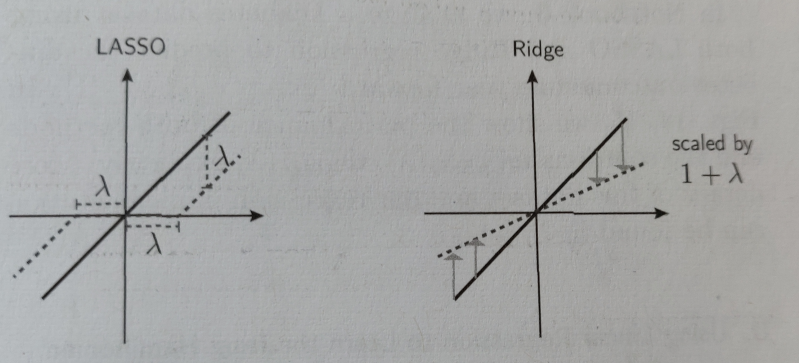
\includegraphics[width=0.7\linewidth]{gfx/LassoVsRidge}
	\caption{}
	\label{fig:lassovsridge}
\end{figure}
\begin{mybox}{On the hyperparameter}
	The regularization parameter $\lambda$ affects the weights (features) the model (LASSO, Ridge) learns on a data set.
\end{mybox}

\subsubsection{A note on LASSO and Ridge}
Note that both LASSO and Ridge regression are convex in  $\mw$ . What's more, Ridge is actually a strictly convex problem (assuming  $\lambda >0$ ) due to presence of $L_2$ penality. In fact, this is always true regardless of  $\mX$  and so the ridge regression solution is always well-defined.

In contrast, LASSO is not always strictly convex and hence by convexity theory, it need not have a unique solution. The LASSO solution is unique under general conditions, for example, when  $\mX$  has columns in general position. To mitigate this, one can define a modified problem called the elastic net such that the function we want to minimize is always strictly convex:
\bse 
\min_{\mw \in \mR^p}\norm{\mX \mw -\my}^2_2 + \lambda \norm{\mw}_1+\delta \norm{\mw}^2_2
\ese 
where  $λ,δ\geq 0$  are regularization parameters. Now aside from uniqueness of the solution, the elastic net combines some of the desirable properties (e.g. prediction) of ridge regression with the sparsity properties of the LASSO.
\subsubsection{Another note being a general comment on regularization}
Comparing the performance of OLS, LASSO and Ridge for the $1D$ Ising model via the coefficient of determination \ref{eq:errorR2} by looking at the parameter space of the hyperparameter $\lambda$, one can draw the following conclusions.\\
Choosing whether to use Ridge or LASSO regression turns out to be similar to fixing gauge degrees of freedom.
\begin{mybox}{Picking a regularization scheme}
	Different regularization schemes can lead to learning equivalent models but in different ’gauges’. Any information we have about the symmetry of the unknown model that generated the data should be reflected in the definition of the model and the choice of regularization.
\end{mybox}

\subsubsection{A general perspective on regularizers}
\begin{mybox}{On the hyperparameter}
	The \textbf{hyperparameter} $\lambda$ involved in e.g. LASSO and Ridge is usually predetermined, which means that it is not part of the regression process. Our learning performance and solution depends strongly on $\lambda$, thus it is vital to choose it properly. As discussed in \ref{subsec:priors}, one approach is to assume an \emph{uninformative prior} on the hyper-parameters, $p(\lambda)$, and average the posterior over all choices of $\lambda$ following this distribution. However, this comes with a large computational cost. Therefore, is is simpler to choose the regularization parameter through some optimization procedure.
\end{mybox}






\subsection{Bayesian formulation of linear regression}
\label{subsec:lregBayesian}
In the formal statistical treatment of regression, the goal is to estimate the \emph{conditional expectation} of the depndent variable given the value of the independent variable (sometimes called the covariate). To connect linear regression to the Bayesian framework, we use \ref{eq:bayesianFreqConnectionModel}. In combination with \ref{eq:bayesLogLikelihood}, we get
\bse 
l(\mt)=-\frac{1}{2\sigma^2} \sum_{i=1}^n(y_i-\mw^T \mx^{(i)})^2-\frac{n}{2} \log(2 \pi  \sigma^2) = -\frac{1}{2\sigma^2} \norm{\mX \mw -\my}^2_2 + const.
\ese
\begin{mybox}{} 
By comparing this with \ref{eq:lregOLSsolution}, it is clear that 
 performing least squares is the same as maximizing the log-likelihood of this model.
\end{mybox}

 \subsubsection{Regularization }
 What about adding regularization?
 \begin{mybox}{}
 The MAP estimate  \ref{eq:bayesMAPestimate} corresponds to regularized linear regression, where the choice of prior determines the type of regularization.
 \end{mybox}
The equivalence between MAP estimation with a Gaussian prior and Ridge regression is established by comparing \ref{eq:bayesMAPestimatorGaussianPrior} and Ridge regression \ref{eq:lregRidgeSol} with $\lambda \equiv \sigma^2/\tau^2$. An analogous derivation holds for LASSO \todo{todo ?}.

\subsection{Outlook from linear regression}
Linear regression can be applied to model non-linear relationships between input and response. This can be done by replacing the input $\mx$ with some non-linear function $\phi(\mx)$. Note that doing so preserves the linearity as a function of the parameters $\mw$, since the model is defined by their inner product $\phi^T(\mx) \mw$. This method is known as \emph{basis function expansion}.\footnote{Look into ML for physicists review for references.}







\section{Logistic Regression}
\label{sec:logisticRegression}
So far we have focused on learning from datasets for which there is a ’continuous’ output. However, a wide variety of problems, such as \emph{classification}, are concerned with outcomes taking the form of discrete variables (i.e. \emph{categories}).
\begin{example}
	For example, we may want to detect if there is a cat or a dog in an image.
\end{example}
We will now introduce \emph{logistic regression} which deals with binary, dichotomous outcomes (.e.g. True or False, Success or Failure,etc.).
\subsection{Mathematical set-up}
\subsubsection{Binary classification}
\label{subsubsec:classBinary}
Throughout this section, we consider the case where the dependent variables $y_i\in \Z$ are discrete and only take values from $m=0,\dots,M-1$ (which enumerate the $M$ classes). The goal is to predict output classes from the design matrix $\mX\in \mR^{n\times  p}$ made of $n$ samples, each of which bears $p$ features. The primary goal is to identify the classes to which new unseen samples belong.
\subsubsection{Multi-class classification}
\label{subsubsec:classMultiClass}
For multi-class classification, we can not only look at binary classification (in which the labels are dichotomous variables). One approach is to treat the label as a vector $\my_i\in \Z^M_2$, namely a binary string of length $M$ with only one component of $y_i$ being $1$ and the rest zero.
\begin{example}
	For example, $\my_i=(1,0,\dots,0)$ means data the sample $\mx_i$ belongs to class $1$.
\end{example}




\subsection{Classifiers}
Given $\mx_i$, the classifier returns the probability of being in category $m$. The following perceptron is an example of \emph{hard} classification, each datapoint is assigned to a category (i.e. $y_i=0$ or $y_i=1$). A \emph{soft} classifier on the other hand gives the probability of a given category as an output.\\
The classifiers do this by using threshold functions, which are discussed in the following \ref{subsubsec:thresholdfct}.\\
In many cases, it is favourable to work with a soft classifier.
\subsubsection{On threshold function functions}
\label{subsubsec:thresholdfct}
	A threshold function is a function that maps its input $\mx$ (a real-valued vector) to an output value $f(x)$ (a single binary value).
One simple way to get a discrete output is to have sign (or threshold) functions that map the output of a linear regressor to $\{0,1\}$. The following are possible:
\begin{enumerate}
	\item Step functions (perceptrons) given by the \emph{sign} function 
\be
\label{eq:logRegsign}
\sigma(s_i)=\text{sign}(s_i)= \left\{\begin{array}{ll}
	1 & \text{if } s_i\geq 0 \\
	0 & \text{otherwise} \\
\end{array}  \right\}
\ee
are employed for hard classification.
\item The \emph{logistic} (or \emph{sigmoid}) function (i.e. Fermi functions)
\be 
\label{eq:logRegSigmoid}
\sigma(s) = \frac{1}{1+e^{-s}}, \quad 1-\sigma(s) = \sigma(-s).
\ee 
\item The hyperbolic tangent 
\todo{Put definition here}
\be 
\label{eq:logRegHyperbolicTangent}
\tanh(z) 
\ee 
\item Rectified linear units (ReLUs) 
\item Leaky rectified linear unity (leaky ReLUs)
\item Exponential linear units (ELUs)
\end{enumerate} 














\subsection{Perceptron Learning Algorithm (PLA)}
Before delving into the details of logistic regression, it is helpful to consider a slightly simpler classifier.
\begin{mybox}{Perceptron crude idea}
	Consider a linear classifier that categorizes examples using a weighted linear-combination of the features and an additive offset:
	\be 
	\label{eq:logRegPerceptron}
	s_i = \mx^T_i \mw + b_0  \equiv \mathbf{\tx}^T_i \mathbf{\tw},
	\ee 
	where we use the short-hand notation $\mathbf{\tx}_i=(1,\mx_i)$ and $\mathbf{\tw}=(b_0,\mw)$. This function takes values on the entire real axis. IN the case of logistic regression, however, the labels $y_i$ are discrete variables. Using the sign function \ref{eq:logRegsign} to create discrete outputs via hard classification, we obtain the \emph{perceptron} model.\\
	In the modern sense, the perceptron is an algorithm for learning a binary classifier called a  \emph{threshold function}, see \ref{subsubsec:thresholdfct}.
\end{mybox}
\subsubsection{The algorithm}


Suppose that we're given a set of $N$ observations each bearing $p$ features, $\mx_n=(x_1^{(n)},\cdots, x_p^{(n)})\in\mathbb{R}^p$, $n=1,\cdots, N$. The goal of binary classification is to relate these observations to their corresponding binary label $y_n \in\{+1,-1\}$. Concretely, this amounts to finding a function $h: \mathbb{R}^p\rightarrow \{+1,-1\}$ such that $h(\mx_n)$ is ideally the same as $y_n$. 
\begin{mybox}{Perceptron} 
	A \emph{perceptron} accomplishes this feat by utilizing a set of weights $\tw=(w_0,w_1,\cdots, w_d)\in\mathbb{R}^{p+1}$ to construct $h$ so that labelling is done through
\be 
	h(\tx_n)=\text{sign }\left(w_0+\sum_{i=1}^p w_ix_i^{(n)}\right) =\text{sign }(\tw^T\tx_n),
	\ee 
	
	where $\tx_n=(1,x_1^{(n)},\cdots, x_p^{(n)}) = (1,\mx_n)$. The perceptron can be viewed as the zero-temperature limit of the logistic regression where the sigmoid (Fermi-function) becomes a step function.
	
\end{mybox}

PLA begins with randomized weights. It then selects a point from the training set at random. If this point, say, $\tx_n$, is misclassified, namely, $y_n\neq \text{sign }(\tw^T\tx_n)$, weights are updated according to 
\be 
\tw\leftarrow \tw+ y_n\tx_n
\ee 
Otherwise, $\tw$ is preserved and PLA moves on to select another point. This procedure continues until a specified threshold is met, after which PLA outputs $h$. It is clear that PLA is an online algorithm since it does not treat all available data at the same time. Instead, it learns the weights as it progress along data points in the training set one-by-one. The update rule is built on the intuition that whenever a mistake is encountered, it corrects its weights by moving towards the right direction. 












\subsection{Definition of logistic regression - Bayesian}
This is a binary classification problem, see \ref{subsubsec:classBinary}.
Here we define logistic regression and discuss the minimization of its corresponding cost function (the \emph{cross entropy}). 
\begin{mybox}{Logistic regression}
	Logistic regression is the canonical example of a soft classifier. In logistic regression, the probability that a data point $\mx_i$ belongs to a category $y_i = \{0,1\}$ is given by 
	\begin{align*}
		P(y_i=1|\mx_i,\mt)&= \frac{1}{1+e^{-\mathbf{\tx}^T_i \mt}} = \sigma(\mathbf{\tx}^T_i \mathbf{\tw})\\
		P(y_i=0|\mx_i,\mt) &= 1-P(y_i=1|\mx_i,\mt)
	\end{align*}
	where $\mt = \mathbf{\tw}$ are the weights we wish to learn from the data. The cost function of logistic regression, the \emph{cross entropy}, is found to be
	\be 
	\label{eq:logregCrossEntropy}
	\mC(\mathbf{\tw} )= \sum_{i=1}^n \left[-y_i \log \sigma(\mathbf{\tx}^T_i \mathbf{\tw}) -(1-y_i) \log\left(1-\sigma(\mathbf{\tx}^T_i \mathbf{\tw})\right)\right].
	\ee 
	In practice, we usually implement the cross-entropy (like in linear regression) with additional regularization terms, usually $L_1$ and $L_2$ regularization.
\end{mybox}
\begin{mybox}{Minimizing the cross entropy}
	The cross entropy is a convex function of the weights $\tw$ and, therefore, any local minimizer is a global minimizer. Minimizing this cost function leads to 
	\be 
	\label{eq:logregCrossEntropyMinimized}
	0 = \mathbf{\nabla} \mC(\tw) = \sum_{i=1}^n \left[\sigma(\tx^T_i \tw) - y_i\right]\tx_i.
	\ee 
	In words, the gradient points in the sum of training example directions weighted by the difference between the true label and the probability of predicting that label.
	Equation \ref{eq:logregCrossEntropyMinimized} defines a transcendental equation for $\tw$, the solution of which, unlike linear regression, cannot be written in a closed form. For this reason, one must use numerical methods such as \ref{sec:gd} to solve this optimization problem.
\end{mybox}\footnote{However, as a word of caution, note there is a generic instability in the MLE procedure for linearly separable data)}
In the notebooks, one looks at two examples to train a logistic regressor to classify binary data.
We call \emph{one-hot} a group of bits where only one bit is $1$ and all others $0$, i.e. representing states: $\ket{1}=(1,0,\dots,0), \ket{2}=(0,1,0,\dots,0)$.
\subsubsection{On the 2d Ising example}
Given an Ising state, we would like to classify whether it belongs to the ordered or the disordered phase, without any additional information other than the spin configuration itself. This categorical ML problem is well suited for logistic regression, and will thus consist of recognizing whether a given state is ordered by looking at its bit configurations. Notice that, for the purposes of logistic regression, the $2D$ spin state of the Ising model will be flattened out to a $1D$ array, so it will not be possible to learn information about the structure of the contiguous ordered $2D$ domains. SUch information can be incorporated using deep convolutional neural networks.\\
We use both ordered and disordered states to train the logistic regressor and, once the supervised training procedure is complete, we will evaluate the performance of our classification model on unseen ordered, disordered, and near-critical states. Here, we deploy the \emph{liblinear} routine (the default for Scikit' s logistic regression) and stochastic gradient descent to optimize the logistic regression cost function with $L_2$ regularization. We define the accuracy of the classifier as the percentage of correctly classified data points. Comparing the accuracy on the training and test data, we can study the degree of overfitting.\\
Similar to the linear regression examples, we find that there exists a sweet spot for the SGD regularization strength $\lambda$ that results in optimal performance of the logistic regressor.
\subsubsection{SUSY }
Here we will use logistic regression in an attempt to find the relative probability that an event is from a signal or a background. Is a good classification problem with noisy data, how to discriminate against the background ? Some signal events look background-like, and some background events look signal-like to our discriminator.
\subsection{SoftMax regression}
\label{subsec:logregSoftMax}
In this section we generalize logistic regression to the case of multiple categories which is called \emph{SoftMax regression}. This is a multi-class classification problem \ref{subsubsec:classMultiClass}.\\
For general categorical data, $y$ can then take on $M$ values so that $y\in \{0,1,\dots, M-1 \}$. For each datapoint $i$, define a vector $y_{im} \equiv [\my_i]_{m}$, whichs refers to the $m^\prime$-th component of vector $\my_i$, called a \emph{one-hot} vector, such that
\be
y_{im} = \left\{ \begin{array}{ll}
	1, & \text{if } y_i = m \\
	0, & \text{otherwise}. \\
\end{array}	\right\}
\ee 
\begin{mybox}{SoftMax regression}
	The probability of $\mx_i$ being in class $m^\prime$ is given by
	\be
	\label{eq:logregSoftMaxfct} 
	\hat{y}_{im (\tw) = p(yi=m^\prime | \tx_i;\tw) \equiv }P(y_{im^\prime} =1 | \mx_i,\{\tw_k\}^{M-1}_{k=0})=\frac{e^{-\tx^T_i \tw_{m^\prime}}}{\sum_{m=0}^{M-1} e^{-\tx^T_i \tw_m}},
	\ee 
	where $y_{im^\prime} \equiv [\my_i]_{m^\prime}$ refers to the $m^\prime$-th component of vector $\my_i$. This is known as the \emph{SoftMax} function. The generalized cost function reads
	\begin{align}
	\label{eq:logregSoftMaxcostFct}
	\mC(\tw) &= - \sum_{i=1}^n \sum_{m=0}^{M-1} \left[ y_{im} \log P(y_{im}=1|\mx_i, \tw_m) \right.. \\
	&\left. + (1-y_{im }) \log\left(1-P(y_{im} =1 |\mx_i ,\tw_m)\right)\right],
	\end{align} 
	which reduces to the cross entropy \ref{eq:logregCrossEntropy} for $M=1$, i.e. for only two possible classes.
\end{mybox}




\section{Ensemble Methods - On combining models}
\label{sec:ensembles}
\subsection{Introduction}
Ensemble methods combine predictions from multiple, often weak, statistical models to improve predictive performance. Ensemble methods, such as random forests, and boosted gradient trees, such as XGBoost, undergird many of the winning entries in data science competitions such as Kaggle, especially on structured datasets. Note that Neural Networks generally perform better than ensemble methods on unstructured data, images and audio. Even in the context of NN, it is common to combine predictions from multiple neural networks to increase performance on tough image classification tasks.
\subsubsection{Motivation}
\label{subsubsec:ensemblesMotivation}
We will give an overview of ensemble methods and provide rules of thumb for when and why they work.\\
On one hand, the idea of training multiple models and then using a weighted sum of the predictions of all these models is very natural. On the other hand, one can also imagine that the ensemble predictions can be much worse than the predictions from each of the individual models that constitute the ensemble, especially when pooling reinforces weak but correlated deficiencies in each of the individual predictors. Thus, it is important to understand when we expect ensemble methods to work.\\
As we saw in \ref{subsubsec:biasvarianceMathematicalEnsemble}, the key to determining when ensemble methods work is the degree of correlation between the models in the ensemble.
\subsubsection{Benefits of Ensemble Methods before diving in}
Three distinct shortcomings that are fixed by ensemble methods are: statistical, computational, and representational.\\
The first reason is statistical. When the learning set is too small, a learning algorithm can typically find several models in the hypothesis space $\mH$ that all give the same performance on the training data. Provided their predictions are uncorrelated, averaging several models reduces the risk of choosing the wrong hypothesis. The second reason is computational. Many learning algorithms rely on some greedy assumption or local search that may get stuck in local optima. As such, an ensemble made of individual models built from many different starting points may provide a better approximation of the true unknown function than any of the single models. Finally, the third reason is representational. In most cases, for a learning set of finite size, the true function cannot be represented by any of the candidate models in $\mH$. By combining several models in an ensemble, it may be possible to expand the space of representable functions and to better model the true function.\\
\\ 
The increase in representational power of ensembles comes from the fact that it is more advantageous to combine a group of simple hypotheses than to utilize a single arbitrary linear classifier. This of course comes with the price of introducing more parameters to our learning procedure. But if the problem itself can never be learned through a simple hypothesis, then there is no reason to avoid applying a more complex model. Since ensemble methods reduce the variance and are often easier to train than a single complex model, they are a powerful way of increasing representational power (also called expressivity in the ML literature).\\
\\
How should we construct ensembles ?\\
\begin{enumerate}
	\item Try to randomize ensemble construction as much as possible to reduce the correlations between predictors in the ensemble. This ensures that our variance will be reduced while minimizing an increase in bias due to correlated errors.
	\item The ensembles will work best for procedures where the error of the predictor is dominated by the variance and not the bias. Thus, these methods are especially well suited for unstable procedures whose results are sensitive to small changes in the training dataset.
	\item Although the discussion above was derived in the context of continuous predictors such as regression, the basic intuition behind ensembles applies equally well to classification tasks. Using an ensemble allows one to reduce the variance by averaging the result of many independent classifiers. As with regression, this procedure works best for unstable predictors for which error are dominated by variance due to finite sampling rather than bias.
\end{enumerate}


\subsection{Aggregate predictor methods - Bagging and Boosting}
A powerful approach is the idea to build a strong predictor by combing many weaker classifiers from different models.
In bagging, the contribution of all predictors is weighted equally in the bagged (aggregate) predictor \ref{eq:ensemblesBaggingaggregatePredictorcontinuous}. However, in principle, there are myriad ways to combine different predictors. In some problems one might prefero to use an autocratic approach that emphasizes the best predictors, while in others it might be better to opt for more ’democratic’ ways as is done in bagging, compare \ref{subsubsec:ensemblesBagging}. In boosting on the other hand, one associates weights to the different weak classifiers in order to amplify the contribution from the most robust classifiers, compare \ref{subsubsec:ensemblesBoosting}.
\subsubsection{Bagging}
\label{subsubsec:ensemblesBagging}
BAGGing, or Bootstrap AGGregation, is one of the most widely employed and simplest ensemble-inspired methods.
Bagging is effective on ’unstable’ learning algorithms where small changes in the training set result in large changes in predictions.\\
Imagine we have a very large dataset $\mL$ that we could partition into $M$ smaller data sets which we label $\{\mL_1,\dots,\mL_m\}$. If each partition is sufficiently large to learn a predictor, we can create an ensemble aggregate predictor composed of predictors trained on each subset of the data. For continuous predictors like regression, this is just the average of all the individual predictors 
\be 
\label{eq:ensemblesBaggingaggregatePredictorcontinuous}
\hat{g}^A_{\mL}(\mx) = \frac{1}{M} \sum_{i=1}^M g_{\mL_i} (\mx).
\ee 
For classification tasks where each predictor predicts a class label $j\in \{1,\dots,J\}$, this is just a majority vote of all the predictors,
\be 
\label{eq:ensemblesBaggingaggregatePredictorclassification}
\hat{g}^A_{\mL}(\mx) = \arg \max_j \sum_{i=1}^M I[g_{\mL_i}(\mx)=j],
\ee 
where $I[]$ is an indicator function that is equal to one if $g_{\mL_i}(\mx)=j$ and zero otherwise. \\
\begin{mybox}{}
	This can significantly reduce the variance without increasing the bias.
\end{mybox}
While simple and intuitive, this form of aggregation clearly works only when we have enough data in each partitioned set $\mL_i$. To see this, one can consider the extreme limit where $\mL_i$ contains exactly one point. In this case, the bases hypothesis $g_{\mL_i}(\mx)$ (e.g. linear regressor) becomes extremely poor and the procedure above fails. One way to circumvent this shortcoming is to resort to \emph{empirical bootstrapping}, which is treated in more detail in \ref{subsubsec:ensemblesBootstrapping}. The idea of empirical bootstrapping is to use sampling with replacement to create new ’bootstrapped’ datasets $\{L^{BS}_1,\dots,L^{BS}_M\}$ from our original dataset $\mL$. These bootstrapped datasets share many points, but due to the sampling with replacement, are all somewhat different from each other. 
\begin{mybox}{Bootstrapped Bagging}
	In the bagging procedure, we create an aggregate estimator by replacing the $M$ independent datasets by the $M$ bootstrapped estimators
	\be 
	\label{eq:ensemblesBaggingBSaggregatePredictorcontinuous}
	\hat{g}^{BS}_{\mL} (\mx) = \frac{1}{M} \sum_{i=1}^M g_{\mL^{BS}_i} (\mx),
	\ee
	and 
	\be 
	\label{eq:ensemblesBaggingBSaggregatePredictorclassification}
	\hat{g}^{BS}_{\mL}(\mx) = \arg\max_j \sum_{i=1}^M I[g_{\mL^{BS}_i} (\mx) = j].
	\ee 
	This bootstrapping procedure allows us to construct an approximate ensemble and thus reduce the variance. For unstable predictors, this can significantly improve the predictive performance. The price we pay for using bootstrapped training datasets, as opposed to really partitioning the dataset, is an increase in the bias of our bagged estimators.
\end{mybox}
\begin{mybox}{Limitations of Bagging}
When the procedure is unstable, the prediction error is dominated by the variance and one can exploit the aggregation component of bagging to reduce the prediction error. In contrast, for a stable procedure the accuracy is limited by the bias introduced by using bootstrapped datasets. This means that there is an instability-to-stability transition point beyond which bagging stops improving our prediction.
\end{mybox}
For more complicated datasets, how can we choose the right hyperparameters?
\begin{mybox}{Out-of-bag estimate and out-of-bag prediction error}
We can actually make use of one of the most important and interesting features of ensemble methods that employ Bagging: \emph{out-of-bag} (OOB) estimates. Whenever we bag data, since we are drawing samples with replacement, we can ask how well our classifiers do on data points that are not used in the training. This is the \emph{out-of-bag prediction error} and plays a similar role to cross-validation error in other ML methods. Since this is the best proxy for out-of-sample prediction, we choose hyperparameters to minimize the out-of-bag error.
\end{mybox}
This is listed in \ref{subsubsec:bayesOOBestimators} for reference, will have to expand on it.












\subsubsection{Boosting}
\label{subsubsec:ensemblesBoosting}
 \begin{mybox}{Boosting}
 	In boosting, an ensemble of weak classifiers $\{g_k(\mx)\}$ is combined into an aggregate, boosted classifier. However, unlike bagging \ref{subsubsec:ensemblesBagging}, each classifier is associated with a weight $\alpha_k$ that indicates how much it contributes to the aggregate classifier
 	\be 
 	\label{eq:ensemblesBoostingAggregateClassifier}
 	g_A(\mx) = \sum_{k=1}^M \alpha_k g_k(\mx),
 	\ee 
 	where $\sum_k \alpha_k =1$. Boosting, like all ensemble methods, works best when we combine simple, high-variance classifiers into a more complex whole.
 \end{mybox}
There are different ideas of how the boosting itself works, for now we only discuss \emph{adaptive boosting} or AdaBoost. The basic idea is to form the aggregate classifier in an iterative process. Importantly, at each iteration we reweight the error function to ’highlight’ data points where the aggregate classifier performs poorly (so that in the next round the procedure puts more emphasis on making those right.) In this way, we can successively ensure that our classifier has good performance over the whole dataset.\\
How does AdaBoost work ?\\
Suppose that we are given a data set $\mL=\{(\mx_i,y_i),i=1,\dots,N\}$ where $\mx_i \in \mathcal{X}$ and $y_i\in\mathcal{Y}=\{+1,-1\}$. Our objective is to find an optimal hypothesis/classifier $g:\mathcal{X}\rightarrow \mathcal{Y}$ to classify the data. Let $\mH=\{g:\mathcal{X}\rightarrow \mathcal{Y}\}$ be the family of classifiers available in our ensemble. In the AdaBoost setting, we are concerned with the classifiers that perform somehow better than ’tossing a fair coin’. This means that for each classifier, the family $\mH$ can predict $y_i$ correctly at least half of the time.\\
We construct the boosted classifier as follows:
\begin{enumerate}
	\item Initialize
	\bse 
	w_{t=1}(\mx_n)=\frac{1}{N},\quad n=1,\dots,N.
	\ese 
	\item For $t=1,\dots, T$ (desired termination step) do:
	\begin{enumerate}
		\item Select a hypothesis $g_t \in \mH$ that minimizes the weighted error 
		\be
		\epsilon_t = \sum_{i=1}^N w_t(\mx_i) \mI(g_(\mx_i)\neq y_i).
		\ee 
		\item Let $\alpha_t = \half \ln \frac{1-\epsilon_t}{\epsilon_t}$ update the weight for each data $\mx_n$ by 
		\bse 
		w_{t+1}(\mx_n)\leftarrow w_t(\mx_n) \frac{\exp[-\alpha_t y_n g_t(\mx_n)]}{Z_t},
		\ese 
		where $Z_t=\sum_{n=1}^N w_t(\mx_n) e^{-\alpha_t y_n g_t(\mx_n)}$ ensures all weights add up to unity.
		\item Output
	\bse 
	g_A(\mx) = \text{sign}\left(\sum_{t=1}^T \alpha_t g_t(\mx)\right).
	\ese 
	\end{enumerate}
\end{enumerate}
\subsection{Random Forests}
\label{subsec:ensemblesRandomForest}
We now review one of the most widely used and versatile algorithms in data science and ML, \emph{Random Forests} (RF).
\begin{mybox}{Random Forests}
	Random Forests is an ensemble method widely deployed for complex classification tasks. A random forest is composed of a family of (randomized) tree-based classifier decision trees, cf. \ref{subsubsec:ensemblesRFDecisionTree}.
\end{mybox}
In order to create an ensemble of decision trees, we must introduce a randomization procedure. The power of ensembles to reduce variance only manifests when randomness reduces correlations between the classifiers within the ensemble, as discussed in \ref{subsubsec:ensemblesMotivation}. Randomness is usually introduced into random forests in one of three distinct ways.
\begin{enumerate}
	\item Use bagging (cf. \ref{subsubsec:ensemblesBagging}) and simply ’\emph{bag}’ the decision trees by training each decision tree on a different bootstrapped dataset. Strictly speaking, this procedure dos not constitute a random forest but rather a bagged decision tree.
	\item Only use a different random subset of the featues at each split in the tree. This \emph{feature bagging} is the distinguishing characteristic of random forests. Using feature bagging reduces correlations between decision trees that can arise when only a few features are strongly predictive of the class label. 
	\item Extremized random forests (ERF) combine ordinary and feature bagging with an extreme randomization procedure where splitting is done randomly instead of using optimality criteria. Even though this reduces the predictive power of each individual decision tree, it still often improves the predictive power of the ensemble because it dramatically reduces correlations between members and prevents overfitting.
\end{enumerate}
\begin{mybox}{Why are they cool}
	RFs are largely immune to overfitting problems even as the number of estimators in the ensemble becomes large. By random selection of input features, random forest improves the variance reduction of bagging by reducing the correlation between the trees without dramatic increase of variance.
\end{mybox}
There are two main hyper-parameters that will be important in practice for the performance of the algorithm and the degree to which it overfits/underfits: the number of estimators in the ensemble and the depth of the trees used. 














\subsection{Gradient Boosted Trees and XGBoost}
\label{subsec:ensemblesGBoostedTreesandXGBoost}
The basic idea of gradient-boosted trees is to use intuition from boosting (cf. \ref{subsubsec:ensemblesBoosting}) and gradient descent (cf. \ref{sec:gd}) to construct ensembles of decision trees (for decision trees, see \ref{subsubsec:ensemblesRFDecisionTree}). Like in boosting, the ensembles are created by iteratively adding new decision trees to the ensembles. 
\begin{mybox}{Gradient Boosted Trees - Essence}
In gradient boosted trees, one critical component is a cost function that measures the performance of our ensemble. At each step, we compute the gradient of the cost function w.r.t. the predicted value of the ensemble and add trees that move us in the direction of the gradient. 
\end{mybox}
Of course, this requires a clever way of mapping gradients to decision trees, this is done within XGBoost (Extreme Gradient Boosting) \ref{subsubsec:ensemblesXGBoost}
\subsubsection{XGBoost}
\label{subsubsec:ensemblesXGBoost}
What follow is a rough sketch of the XGBoost algorithm.\\
Our starting point is a clever parametrization of decision trees. Here, we use notation where the decision tree makes continuous predictions (regression trees), though this can also be generalized to classification tasks. We parametrize a decision tree $j$, denoted as $g_j(\mx)$ with $T$ leaves by two quantities: a function $q: \mx \in \mR^d \rightarrow \{1,2,\dots, T\}$ that maps each data point to one of the leaves of the tree and a weight vector $\mw \in \mR^T$ that assigns a predicted value to each leaf. In other words, the $j$-th decision tree's prediction for the data point $\mx_i$ is simply $g_j(\mx_i) = w_{q(\mx_i)}$.\\
In addition to a parametrization of decision trees, we also have to specify a cost function which measures predictions. The prediction of our ensemble for a datapoint $(y_i,\mx_i)$ is given by
\bse 
\hat{y}_i = g_A(\mx_i) = \sum_{j=1}^M g_j(\mx_i), \quad g_j \in \mathcal{F} 
\ese 
where $M$ is the number of members of the ensemble, and $\mathcal{F}=\{g(\mx) = w_{q(\mx)} \}$ is the space of trees. As discussed for \ref{subsubsec:ensemblesRFDecisionTree}, we introduce a regularization term into the cost function to prevent overfitting.
\begin{mybox}{Cost function XGBoost}
	The cost function is composed of two terms, a term that measures the goodness of predictions on each datapoint, $l_i(y_i,\hat{y}_i)$, which is assumed to be differentiable and convex, and for each tree in the ensemble, a regularization term $\Omega(g_j)$ that does not depend on the data 
	\be 
	\label{eq:ensemblesXGBoostCostfct}
	\mC (\mX,g_A) =\sum_{i=1}^N l(y_i,\hat{y}_i) + \sum_{j=1}^M \Omega(g_j),
	\ee 
	where the index $i$ runs over data points and the index $j$ runs over decision trees in our ensemble. In XGBoost, the regularization function is chosen to be
	\be 
	\Omega(g) = \gamma T + \frac{\lambda}{2}\norm{\mw}^2_2,
	\ee 
	with $\gamma$ and $\lambda$ regularization parameters that must be chosen appropriately. Notice that this regularization penalizes both large weights on the leaves (similar to $L^2$-regularization) and having large partitions with many leaves.
\end{mybox}
As in boosting, we form the ensemble iteratively. For this reason, we define a family of predictors $\hat{y}^{(t)}_i$ as 
\be 
\hat{y}^{(t)}_i = \sum_{j=1}^t g_j(\mx_i) = \hat{y}^{(t-1)}_i + g_t(\mx_i).
\ee
Note that by definition $y^{(M)}_i=g_A(\mx_i)$. 
\begin{mybox}{}
The central idea is that for large $t$, each decision tree is a small perturbation to the predictor (of order $1/T$) and hence we can perform a Taylor expansion on our loss function to second order
\be 
\mC_t =\sum_{i=1}^N l(y_i,\hat{y}^{(t-1)}_i + g_t(\mx_i)) + \Omega(g_t) \approx \mC_{t-1} + \Delta \mC_t,
\ee 
where 
\bse \Delta \mC_t = a_i g_t(\mx_i) + \half b_i g_t(\mx_i)^2 + \Omega(g_t).
\ese 
We then choose the $t$-th decision tree $g_t$ to minimize $\Delta \mC_t$, one finds
\be 
\Delta \mC^{opt}_t = - \half \sum_{j=1}^T \frac{A^2_j}{B_j+\lambda} + \gamma T,
\ee 
where $B_j=\sum_{i\in I_j}b_i, A_j = \sum_{i\in I_j} a_i$, with the set of points that get mapped to leaf $j$ $I_j = \{i | q_t(\mx_i)=j \}$.
\end{mybox}
It is clear that $\Delta \mC^{opt}_t$ measures the in-sample performance of $g_t$ and we should find the decision tree that minimizes this value. In principle, one could enumerate all possible trees over the data and find the tree that minimizes $\Delta \mC^{opt}_t$. However, in practice this is impossible. Instead, an approximate greedy algorithm is run that optimizes one level of the tree at a time by trying to find optimal splits of the data. This leads to a tree that is a good local minimum of $\Delta\mC^{opt}_t$ which is then added to the ensemble.\\
\\
As a note about the sketch above, in practice additional regularization such as \emph{shrinkage} and \emph{feature subsampling} is used. In addition, there are many numerical and technical tricks used for the approximate algorithm and how to find splits of the data that give good decision trees.

\begin{mybox}{Fscore}
	One nice feature of ensemble methods such as XGBoost is that they automatically allow us to calculate feature scores (\emph{Fscores}) that rank the importance of various features for classification. The higher the Fscore, the more important the feature for classification.
\end{mybox}

























\section{An Introduction to Feed-Forward Deep Neural Networks (DNNS)}
\label{sec:dnn}
 Neural networks are one of the most powerful and widely-used supervised learning techniques. Deep Neural Networks (DNNs) got rebranded as ’Deep Learning’ and have become the workhorse technique for many image and speech recognition based ML tasks. The large-scale industrial deplyoment of DNNs has given rise to a number of high-level libraries and packages (Caffe, Keras, Pytorch, Tensorflow, etc.).\\
 Conceptually, it is helpful to divide NNs into four categories 
 \begin{enumerate}
 	\item General purpose NNs for supervised learning,
 	\item NNs designed specifically for image processing, the most prominent example of this class being Convolutional NNs (CNNs), 
 	\item NNs for sequential data such as Recurrent NNs (RNNs), and
 	\item NNs for unsupervised learning such as Deep Boltzmann Machines.
 \end{enumerate}
This section deals with the first two categories.\footnote{Though increasingly important for many applications such as audio and speech recognition, for now we omit a discussion of sequential data and RNNs. Look at \href{https://colah.github.io/posts/2015-08-Understanding-LSTMs/}{Chris Olah's blog} for an introduction to RNNs and LSTM networks.}
Results for modern NNs are largely empirical and heuristic and lack a firm theoretical footing. Therefore, in this review we (for now) only give the fundamentals.

\subsection{Neural Network Basics}
Neural networks (also called neural nets) are neural-inspired nonlinear models for supervised learning. Neural nets can be viewed as natural, more powerful extensions of supervised learning methods such as linear \ref{sec:linearRegression} and logistic regression \ref{sec:logisticRegression} and soft-max methods \ref{subsec:logregSoftMax}.
\subsubsection{The basic building block: neurons}
\label{subsubsec:dnnNeurons}
\begin{mybox}{Neurons}
The basic unit of a neural net is a stylized \emph{neuron} $i$ that takes a vector of $d$ input features $\mx=(x_1,x_2,\dots,x_d)$ and produces a scalar output $a_i(\mx)$. 
\end{mybox}
A neural network consists of many such neurons stacked into layers, with the output of one layer serving as the input for the next. The first layer in the neural net is called the \emph{input layer}, the middle layers are often called \emph{hidden layers}, and the final layer is called the \emph{output layer}.\\
The exact function $a_i$ varies depending on the type of non-linearity used in the NN. However, in essentially all cases $a_i$ can be decomposed into a linear operation that weights the relative importance of the various inputs, and a non-linear transformation $\sigma_i(z)$ which is usually the same for all neurons\footnote{I.e. a threshhold function which squishes the sum of all $a_i$ into a number between $0$ and $1$, cf. \ref{subsubsec:thresholdfct}.}, compare \ref{fig:neuron}. 

\begin{figure}[h!]
	\centering
	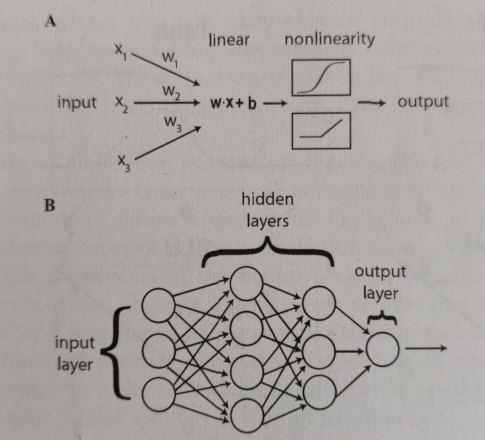
\includegraphics[width=0.7\linewidth]{gfx/Neuron}
	\caption{\itshape A) Neurons consist of a linear transformation that weights the importance of various inputs, followed by a non-linear activation function. B) Network architecture.}
	\label{fig:neuron}
\end{figure}




The linear transformation in almost all NNs takes the form of a dot product with a set of neuron-specific weights $\mw^{(i)} = (w^{(i)}_1,w^{(i)}_2,\dots,w^{(i)}_d)$ followed by re-centring with a neuron-specific bias $b^{(i)}$:
\be 
z^{(i)} = \mw^{(i)} \cdot \mx ü+ b^{(i)} = \tx^T \cdot \tw^{(i)},
\ee 
where $\tx=(1,\mx)$ and $\tw^{(i)} = (b^{(i)}, \mw^{(i)} )$.
\begin{mybox}{Choosing the right non-linearity}
 In terms of $z^{(i)}$ and the non-linear function $\sigma_i(z)$, we can write the full input-output function as 
\be 
\label{eq:dnnInputOutputfct}
a_i(\mx) = \sigma_i ( z^{(i)}).
\ee 
Historical choices of nonlinearities include step-functions (perceptrons), sigmoids (i.e. Fermi functions), and the hyperbolic tangent, cf. \ref{subsubsec:thresholdfct}. More recently, it has become more common to use rectified linear units (ReLUs), leaky rectified linear units (leaky ReLUs), and exponential linear units (ELUs). Different choice of non-linearities lead to different computational and training properties for neurons. The underlying reason for this is that we train neural nets using gd based methods, cf. \ref{sec:gd}, that require us to take derivatives of the neural input-output function with respect to the weights $\mw^{(i)}$ and the bias $b^{(i)}$.
\end{mybox}
Notice that the derivatives of the aforementioned non-linearities $\sigma(z)$ have very different properties. The derivative of the perceptron is zero everywhere except where the input is zero. This discontinuous behaviour makes it impossible to train perceptrons using gradient descent. For this reason, until recently the most popular choice of non-linearity was the $\tanh$ function or a sigmoid/Fermi function. However, this choice of non-linearity has a major drawback. When the input weights become large, as they often do in training, the activation functions saturates and the derivative of the output w.r.t. the weights tends to zero since $\partial \sigma /\partial z \rightarrow 0$ for $z\gg 1$. Such \emph{vanishing gradients} are a feature of any saturating function, making it harder to train deep networks. In contrast, for a non-saturating function such as ReLUs or ELUs, the gradients stay finite even for large inputs.

\subsubsection{Layering neurons to build deep networks: network architecture}
\label{subsubsec:dnnNetworkArchitecture}
The basic idea of all NNs is to layer neurons in a hierarchical fashion, the general structure of which is known as the \emph{network architecture}, compare \ref{fig:neuron}. In the simplest feed-forward networks, each neuron in the \emph{input layer} of the neurons takes the inputs $\tx$ and produces an output $a_i(\tx)$ that depends on its current weights, see \ref{eq:dnnInputOutputfct}. The outputs of the input layer are then treated as the inputs to the next \emph{hidden layer}. This is usually repeated several times until one reaches the top or \emph{output layer}.
\begin{mybox}{Output layer and general architecture}
	The output layer is almost always a simple classifier of the form discussed before: a logistic regression \ref{sec:logisticRegression} or soft-max function \ref{subsec:logregSoftMax} in the case of categorical data (i.e. discrete labels) or a linear regression \ref{sec:linearRegression} layer in the case of continuous outputs. Thus, the whole neural network can be though of as a complicated nonlinear transformation of the inputs $\tx$ into an output $\hat{y}$ that depends on the weights and biases of all the neurons in the input, hidden, and output layers.
\end{mybox}
The use of hidden layers greatly expands the representation power (\emph{expressivity}) of a NN when compared with a simple soft-max or linear regression network, this is exemplified by the following theorem.
\begin{mybox}{Universal approximation theorem}
	A NN with a single hidden layer can approximate any continuous multi-input/multi-output function with arbitrary accuracy.
\end{mybox}
What does this mean and where does this come from ?\\
Note that by increasing the number of hidden neurons we can improve the approximation. Suppose we're given a function $f(x)$ which we'd like to compute to within some desired accuracy $ϵ>0$. The guarantee is that by using enough hidden neurons we can always find a neural network whose output $g(x)$ satisfies 
 \bse 
 \abs{g(x)-f(x)} < \epsilon,
 \ese 
  for all inputs $x$.
The approximation of the function works in the following way like a Riemann sum. Basically every pair of neurons in the hidden layer can be combined, via a combination of both weights, into a step function (or a sigmoid function which becomes a step function for large inputs). To be more precise, you can make every activation function into a step function by a clever combination of weights and bias if the activation function satisfies the following properties:\\
We do need to assume that $s(z)$ is well-defined as$z\rightarrow \infty$ and $z\rightarrow -\infty$. These two limits are the two values taken on by our step function. We also need to assume that these limits are different from one another. If they weren't, there'd be no step, simply a flat graph! But provided the activation function $s(z)$ satisfies these properties, neurons based on such an activation function are universal for computation (i.e. they are able to approximate any function). Why this is is described in the following.
\\
 Having $N$ pairs of hidden layer neuron pairs gives you $N$ step function, which you can arrange beside each other, or overlapping. This is basically the approximation of the function. You arrange step functions in such a way that they give you the function in a small section of the interval. Therefore, basically neuron pairs in the hidden layer provide support functions as in analysis, which are step functions approximating the true function for a small part of the interval. Therefore, by simply increasing the number of hidden layer neurons, you increase the number of step functions and decrease their width, resulting in a finer approximation of the function.\\
This makes use of the weighted combination $\sum_j w_j a_j$ output from the hidden neurons, however the function is given by the output layer, i.e. by the output $\sigma(\sum_j w_j a_j +b)$ where $b$ is the bias on the output neuron. How do you make the transition ?\\
The solution is to design a neural network whose hidden layer has a weighted output given by $\sigma^{-1}\circ f(x)$, such that the overall output will be a very good approximation of $\sigma\circ \sigma^{-1} \circ f(x) = f(x)$.
\\
If you have more inputs for one neuron, i.e. a many-input function $f(x_1,x_2,\dots)$, you get more weights, because every input $x_i$ has a weight $w_i$ associated with it which determines how much this input variable should contribute in this particular neuron, where every neuron also has one specific bias associated with it.\\
For two input variables:\\
 You can again create step function but this time in three dimensions (i.e. $x_1,x_2,g(x_1,x_2)$), which are called tower functions. These are constructed by introducing a second hidden layer. A pair of Neurons in the first hidden layer giving us a step-function in one direction can be combined with a pair of neurons giving us a step function in another direction (and so on) to create a tower function by a clever combination of heights of the two neuron pairs and bias of the neuron in the second hidden layer both of these pairs are connected to. Then, you can create any $3$ or $m$ dimensional function by stacking tower functions together. We can also make them as thin as we like, and whatever height we like. As a result, we can ensure that the weighted output from the second hidden layer approximates any desired function of two variables.
In particular, by making the weighted output from the second hidden layer a good approximation to $\sigma^{-1}\circ f$, we ensure the output from our network will be a good approximation to any desired function, $f$.\\
For $m$ input variables you need to have $m$ neuron pairs in the first hidden layer to feed into one respective neuron in the second hidden layer, where the former create all the step functions in the different dimensions by clever combination of parameters and the latter gives the output tower function in the given dimension.\\
For vector-valued functions, you simply compute the components of the vector separately via the above method and then put them into a vector.
\begin{mybox}{Conclusion}
We saw that we can approximate any function with just one hidden layer. Given this, you might wonder why we would ever be interested in deep networks, i.e., networks with many hidden layers. Can't we simply replace those networks with shallow, single hidden layer networks?\\
While in principle that's possible, there are good practical reasons to use deep networks. Deep networks have a hierarchical structure which makes them particularly well adapted to learn the hierarchies of knowledge that seem to be useful in solving real-world problems. Put more concretely, when attacking problems such as image recognition, it helps to use a system that understands not just individual pixels, but also increasingly more complex concepts: from edges to simple geometric shapes, all the way up through complex, multi-object scenes. Deep networks do a better job than shallow networks at learning such hierarchies of knowledge.
\end{mybox}









\subsubsection{Further on network architecture: How many layers is adequate for a problem ?}
\label{subsubsec:dnnBestPracticeArchitecture}
Deep architectures are favourable for learning. Increasing the number of layers increases the number of parameters and hence the representational power of NNs. Indeed, recent numerical experiments suggest that as long as the number of parameters is larger than the number of data points, certain classes of NNs can fit arbitrarily labelled random noise samples. This suggests that large NNs of the kind used in practice can express highly complex function. Adding hidden layers is also thought to allow neural nets to learn more complex features from the data. Work on convolutional networks suggests that the first few layers of a neural network learn simple, ’low-level’ features that are then combined into higher-level, more abstract features in the deeper layers.\\
\\
Choosing the exact network architecture for a NN remains an art that requires extensive numerical experimentation and intuition, and is often times problem-specific. Both the number of hidden layers and the number of neurons in each layer can affect the performance of a NN.
\begin{mybox}{Rule of thumb}
	A general rule of thumb that seems to be emerging is that the number of parameters in the NN should be large enough to prevent underfitting.
\end{mybox}
Empirically, the best architecture for a problem depends on the task, the amount and type of data that is available, and the computational resources at one's disposal. Certain architectures are easier to train, while others might be better at capturing complicated dependencies in the data and learning relevant input features. Finally, there are architectures beyond simple deep, feed-forward NNs.
For example, modern NNs for image segmentation often incorporate ’skip connections’ that skip layers of NN. This allows information to directly propagate to a hidden or output layer, bypassing intermediate layers and often improving performance.

\subsection{Training deep networks}
\label{subsec:dnnTraining}
\begin{mybox}{Training procedure}
	The training procedure is the same as we used for training simpler supervised learning algorithms such as logistic and linear regression, compare \ref{subsec:recipeML}:\\
	Construct a cost/loss function and then use gradient descent to minimize the cost function and find the optimal weights and biases. 
\end{mybox}
NNs differ from these simpler supervised procedures in that generally they contain multiple hidden layers that make taking the gradient computationally more difficult, this will be discussed in more detail via the \emph{backpropagation} algorithm for computing gradients in \ref{subsec:dnnBackpropagation}.\\
\\
Like all supervised learning procedures, the first thing one must do to train a NN is to specify a loss function. Given a data point $(\tx_i,y_i)$, $\tx_i \in \mR^{d+1}$, the NN makes a prediction $\hat{y}_i(\tw)$, where $\tw$ are the parameters of the NN. Recall that in most cases, the top output layer of our NN is either a continuous predictor or a classifier that makes discrete (categorical) predictions. Depending on whether one wants to make continuous or categorical predictions, one must utilize a different kind of loss function.
\begin{enumerate} 
\item For continuous data, the loss functions that are commonly used to train NNs are identical to those used in linear regression:
\begin{enumerate}
	\item One is the mean squared error
	\be 
	\label{eq:dnnCostSquaredError}
	E(\tw) = \frac{1}{n}\sum_{i=1}^n (y_i-\hat{y}_i(\tw) )^2, 
	\ee 
	where $n$ is the number of data points,
	\item and the mean-absolute error (i.e. $L_1$ norm) 
	\be 
	\label{eq:dnnCostAbsoluteError} 
	E(\tw) = \frac{1}{n} \sum_i \abs{y_i - \hat{y}_i(\tw)}.
		\ee 
\end{enumerate}
The full cost function often includes terms that implement regularization (e.g. $L_1$ or $L_2$ regularizers).
\item For categorical data, the most commonly used loss function is the cross-entropy (\ref{eq:logregCrossEntropy} and \ref{eq:logregSoftMaxcostFct}), since the output layer is often taken to be a logistic classifier for binary data with two types of labels, or a soft-max classifier if there are more than two types of labels. As usual, these loss functions are often supplemented by aditional terms that implement regularization.
\end{enumerate}
Having defined an architecture and a cost function, we must now train the model. Similar to other supervised learning methods, we make use of gradient-descend based methods \ref{sec:gd} to optimize the cost function. Recall that the basic idea of GD is to update the parameters $\tw$ to move in the direction of the gradient of the cost function $\nabla_{\tw} E(\tw)$.\footnote{Most modern NN packages, such as Keras, allow the user to specify which of the optimizers discussed in \ref{sec:gd} they would like to use in order to train the NN. Depending on the architecture, data, and computation resources, different optimizers may work better on the problem, though vanilla SGD \ref{subsubsec:gdSGD} is a good first choice.}

\subsection{The Backpropagation algorithm}
\label{subsec:dnnBackpropagation}
The training procedure of a NN requires us to be able to calculate the derivative of the cost function w.r.t. all the parameters of the NN (the weights and biases of all the neurons in the input, hidden, and visible layers). The backpropagation algorithm is a clever procedure that exploits the layered structure of NNs to more efficiently compute gradients.\\
We will assume that there are $L$ layers in our network with $l=1,\dots,L$ indexing the layer. Denote by $w^l_{jk}$ the weight for the connection from the $k$-th neuron in layer $l-1$ to the $j$-th neuron in layer $l$ We denote the bias of this neuron by $b^l_j$. By construction, in a feed-forward NN the activation $a^l_j$ of the $j$-th neuron in the $l$-th layer can be related to the activities of the neurons in the layer $l-1$ by the equation
\be 
\label{eq:dnnBackpropActivation}
a^l_j = \sigma \left(\sum_k w^l_{jk} a^{l-1}_k + b^l_j\right)= \sigma(z^l_j).
\ee
Define the error $\Delta^L_j$ of the $j$-th neuron in the $L$-th layer as the change in cost function w.r.t. the weighted input $z^L_j$ 
\be
\label{eq:dnnBackprop1}
\Delta^L_j=\frac{\partial E}{\partial z^L_j},
\ee 
where $E$ is the cost function which depends directly on the activities of the output layer $a^L_j$ and indirectly on all the activities of neurons in lower layers iteratively via \ref{eq:dnnBackpropActivation}. Equation \ref{eq:dnnBackprop1} therefore asks the question of how much the cost function changes when we change the weighted sum. Equally, the following three equations ask the question of how the cost function changes w.r.t. a change in the bias, weight and activation respectively.
Equation \ref{eq:dnnBackprop1} together with the following three equations
\begin{align}
	\Delta^l_j&= \frac{\partial^E}{\partial z} = \frac{\partial E}{\partial b^l_j}, \label{eq:dnnBackprop2} \\
	\Delta^l_j &= \sum_k \frac{\partial E}{\partial z^{l+1}_k} \frac{\partial z^{l+1}_k}{z^l_j} =\left(\sum_k \Delta^{l+1}_k w^{l+1}_{kj} \right) \sigma^\prime(z^l_j), \label{eq:dnnBackprop3} \\
	\frac{\partial E}{\partial w^l_{jk}} &= \frac{\partial E}{\partial z^l_j} \frac{\partial z^l_j}{\partial w^l_{jk}} = \Delta^l_j a^{l-1}_k.\label{eq:dnnBackprop4}
\end{align}
define the four backpropagation equations relating the gradients of the activations of various neuron $a^l_j$, the weighted inputs $z^l_j=\sum_k w^l_{jk} a^{l-1}_k +b^l_j$, and the errors $\Delta^l_j$. These equations can be combined into a simple, computationally efficient algorithm to calculate th gradient w.r.t. all parameters. As all of them are asking the question of how the error/cost function is affected by a change in one of the parameters, they are  a means of quantifying how to most easily minimize the cost function, compare figure \ref{fig:backpropagation}. This is what the backpropagation algorithm is doing. It combines the average amount of change of the error function w.r.t. one of the parameters into the gradient vector
\bse 
\vec{\nabla} \mC = (w_1,w_2,\dots,w_{1000}, b_1,\dots, b_{400}).
\ese 
The optimized gradient of the cost function is determined via the backpropagation algorithm by choosing the direction of change in this huge parameter space.
\begin{mybox}{The Backpropagation algorithm}
	\begin{enumerate}
		\item \emph{Activation at input layer}:\\
		Calculate the activation $a^1_j$ of all the neurons in the input layer.
		\item \emph{Feedforward}:\\
		Starting with the first layer, exploit the feed-forward architecture through \ref{eq:dnnBackpropActivation} to compute $z^l$ and $a^l$ for each subsequent layer.
		\item \emph{Error at top layer}:\\
		Calculate the error of the top layer using \ref{eq:dnnBackprop1}. This requires to know the expression for the derivative of both the cost function $E(\tw)=E(\textbf{a}^L)$ and the activation function $\sigma(z)$.
		\item \emph{’Backpropagate’ the error}:\\
		Use \ref{eq:dnnBackprop3} to propagate the error backwards and calculate $\Delta^l_j$ for all layers. 
		\item \emph{Calculate gradient}:\\
		Use equations \ref{eq:dnnBackprop2} and \ref{eq:dnnBackprop4} to calculate $\frac{\partial E}{\partial b^l_j}$ and $\frac{\partial E}{\partial w^l_{jk}}$.
	\end{enumerate}
\end{mybox}
The algorithm consists of a forward pass from the bottom layer to the top layer where one calculates the weighted inputs and activations of all the neurons. One then \emph{backpropagates} the error starting with the top layer down to the input layer and uses these errors to calculate the desired gradients. This description makes clear the incredible utility and computational efficiency of the backgpropagation algorithm. We can calculate all the derivatives using a single ’forward’ and ’backward’ pass of the NN. This computational efficiency is crucial since we must calculate the gradient w.r.t. all parameters of the NN at each step of gradient descent.\footnote{These basic ideas also underlie almost all modern automatic differentiation packages such as Autograd (Pytorch).}\\
\begin{figure}[h!]
	\centering
	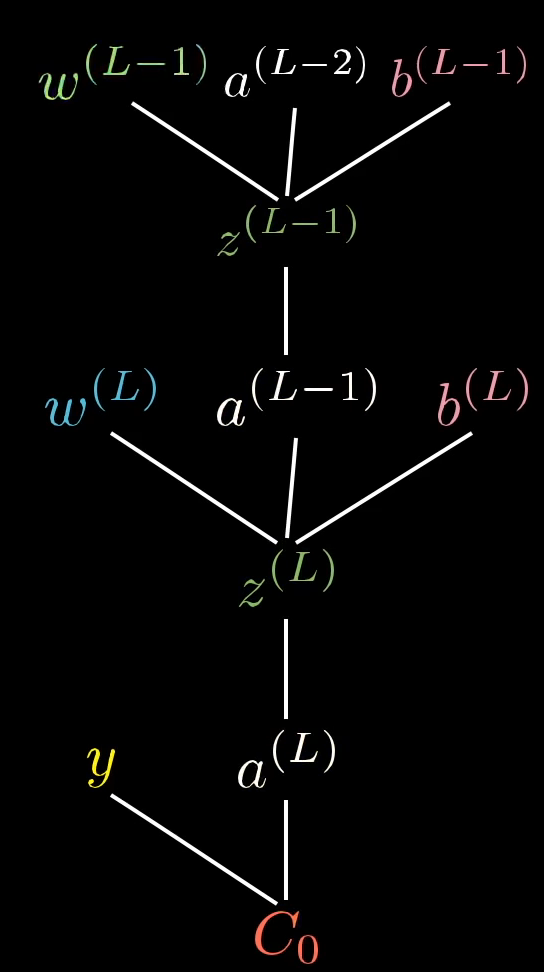
\includegraphics[width=0.3\linewidth]{gfx/Backpropagation}
	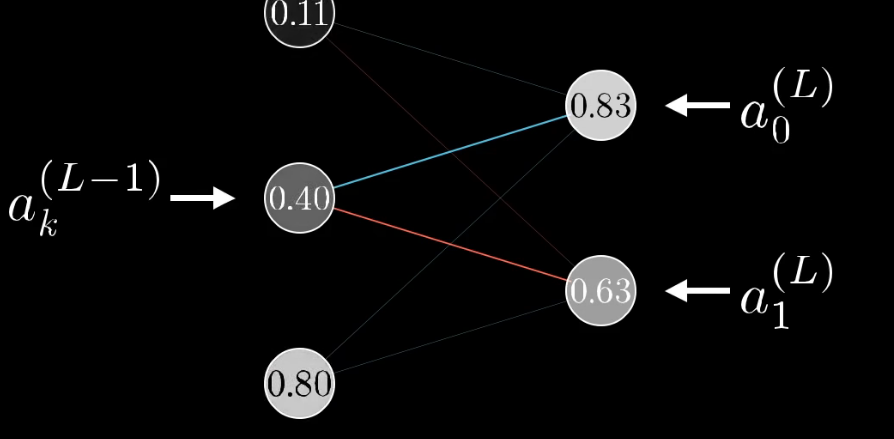
\includegraphics[width=0.6\linewidth]{gfx/Backpropagation2}
	\caption{Left :\itshape Backpropagation for a DNN with one neuron per layer. \normalfont Right: \itshape $L$-th layer is introduced by multiple activations in the previous layer if we have more than one neuron.}
	\label{fig:backpropagation}
\end{figure}
\subsubsection{What can go wrong with backpropagation ?}
\label{subsubsec:dnnBackpropagationProblems}
A problem that occurs in deep networks, which transmit information through many layers, is that gradients can vanish or explode. This is known as the \emph{problem of vanishing or exploding gradients}. Especially pronounced in NNs that try to capture long-range dependencies, such as RNN for sequential data. 
Consider the eigenvalues (or singular values) of the weight matrices $w^l_{jk}$. In order for the gradients to be finite for deep networks, we need these eigenvalues to stay near unity even after many gradient descent steps.\footnote{ In modern feed-forward and ReLU NNs, this is achieved by initializing the weights for the gradient descent in clever ways and using non-linearities that do not saturate, such as ReLUs ( recall that for saturating functions, $\sigma^\prime \rightarrow 0$, which will cause the gradient to vanish).}
Proper initialization and regularization schems such as \emph{gradient clipping} (cutting-off gradients with very large values), and \emph{batch normalization} also help mitigate this problem.\\
Summarizing Backpropagation:\\
Backpropagation is the algorithm for determining how a single training example would nudge all weights and biases of the NN - not in terms of whether they should go up or down but in terms of what relative proportions to those changes cause the \emph{most rapid decrease of the cost function}. A true GD step would involve doing this for all your tens of thousands of training examples and averaging the desired changes that you get (i.e. average change to weight $w_{143}$). This however is computationally slow, such that you randomly subdivide the data into mini-batches and compute each step w.r.t. a mini-batch. Repeatedly going through all the mini-batches making these adjustments to the weights, you will converge towards a local minimum.
\subsection{Regularizing neural networks and other practical considerations}
\label{subsec:dnnRegularizingPractical}
DNNs, like all supervised learning algorithms, must navigate the bias-variance tradeoff \ref{subsubsec:biasvariancetradeoff}.
Regularization techniques play an important role in ensuring that DNNs generalize well to new data. In addition to special regularization techniques (Batch Normalization, Dropout), large DNNs seem especially well-suited to implicit regularization that already takes place in SGD \ref{subsubsec:gdSGD}. The implicit stochasticity and local nature of SGD often prevent overfitting of spurious correlations in the training data, especially when combined with techniques such as Early Stopping.
\subsubsection{Implicit regularization using SGD: Initialization, hyper-parameter tuning, and Early Stopping}
\label{subsubsec:dnnRegularizingPracticalSGDEarlyStopping}
\emph{Implicit regularization using SGD: initialization, hyper-parameter tuning, and Early Stopping}.\\
	The most commonly employed and effective optimizer for training NN is SGD. SGD acts as an implicit regularizer by introducing stochasticity (from the use of mini-batches) that prevents overfitting. 
	\begin{enumerate} 
	\item In order to achieve good performance, it is important that the weight initialization is chosen randomly, in order to break any leftover symmetries. One common choice is drawing the weights from a Gaussian centred around zero with some variance that scales inversely with number of inputs to the neuron. 
	\begin{mybox}{}
		Since SGD is a local procedure, as networks gets deeper, \emph{choosing a good weight initialization becomes increasingly important} to ensure that the gradients are well-behaved.
	\end{mybox}
It is important to experiment with different variances, the NN is extremely sensitive to the choice of variance.
	\item The second important thing is to appropriately choose the learning rate or step-size by searching over five logarithmic grid points. If the best performance occurs at the edge of the grid, repeat this procedure until the optimal learning rate is in the middle of the grid parameters.
	\item Finally, it is common to centre or whiten the input data (as in linreg \ref{sec:linearRegression} and logreg \ref{sec:logisticRegression}).
\end{enumerate}
 Another important form of regularization that is often employed in practice is \emph{Early Stopping}.
\begin{mybox}{Early Stopping}
	The idea of Early Stopping is to divide the training data into two portions, the dataset we train on, and a smaller \emph{validation set} that serves as a proxy for out-of-sample performance of the test set (i.e. cross-validation \ref{subsec:recipeML}, note however that you also split test test into test and play set, where you perform hyperparameter grid search on the play set). As we train the model, we plot both the training error and the validation error (i.e. $E_{in}, E_{out}$). We expect the training error to continuously decrease during training ($E_{in, t} \leq E_{in,t-1}$). However, the validation error will eventually increase due to overfitting. The basic idea of Early Stopping is to halt the training procedure when the validation error starts to rise. This Early Stopping procedure ensures that we stop the training and avoid fitting sample specific features in the data.
\end{mybox}
\subsubsection{Dropout}
\label{subsubsec:dnnRegularizerPracticalDropout}
\begin{mybox}{Dropout}
The basic idea of Dropout is to prevent overfitting by reducing spurious correlations between neurons within the network by introducing a randomization procedure similar to that underlying ensemble models such as Bagging \ref{subsubsec:ensemblesBagging}. Dropout prevents problems of correlation and computational cost by randomly dropping out neurons (along with their connections) from the NN during each step of the training. Typically, for each mini-batch in the GD step, a neuron is dropped from the NN with a probability $p$. The GD step is then performed only on the weights of the ’thinned’ network of individual predictors. Since during training, on average weights are only present a fraction $p$ of the time, predictions are made by reweighing the weights by $p$: $\tw_{test} = p\tw_{train}$. The learned weights can be viewed as some ’average’ weight over all possible thinned NNs, this is similar to Bagging and reduces the variance.
\end{mybox}
\subsubsection{Batch Normalization}
 \label{subsubsec:dnnRegularizerPracticalBatchNorm}
The basic inspiration is that training NNs works best when the inputs are centred around zero w.r.t. the bias. The reason for this is that it prevents neurons from saturating and gradients from vanishing in deep nets.
\begin{mybox}{Batch Normalization}
	The idea of Batch Normalization is to introduce new ’BatchNorm’ layers that standardize the inputs by the mean and variance of the mini-batch. Consider a layer $l$ with $d$ neurons whose inputs are $(z^l_1,\dots,z^l_d)$. We standardize each dimension so that
	\be 
	\label{eq:dnnRegularizerPracticalBatch1}
	z^l_k \rightarrow \hat{z}^l_k = \frac{z^l_k -\mathbb{E}[z^l_k]}{\sqrt{Var[z^l_k]}},
	\ee
	where the mean and variance are taken over all samples in the mini-batch. One furthermore introduces two new parameters $\gamma^l_k, \beta^l_k$ for each neuron that can additionally shift and scale the normalized input
	\be 
	\label{eq:dnnRegularizerPracticalBatch2}
	\hat{z}^l_k \rightarrow \gamma^l_k \hat{z}^l_k + \beta^l_k.
	\ee 
	These two equations \ref{eq:dnnRegularizerPracticalBatch1}, \ref{eq:dnnRegularizerPracticalBatch2} are like adding new extra layers $\hat{z}$ in the deep net architecture.
\end{mybox}
Hence, the new parameters $\gamma^l_k$ and $\beta^l_k$ can be learned just like the weights and biases using backpropagation (since this is just an extra layer for the chain rule). We initiliaze the NN so that at the beginning of training the inputs are being standardized. Backpropagation then adjusts $\gamma,\beta$ during training.\\
In practice, Batch Normalization considerably improves the learning speed by preventing gradients from vanishing. The randomness introduced by the mini-batches seems to shape Batch Normalization as a power regularization tool by introducing additional randomness into the training procedure.

\subsection{Deep neural networks in practice}
\label{subsec:dnnPractice}
Different packages:
\begin{enumerate} 
	\item In Tensorflow one constructs data flowgraphs, the nodes of which represent mathematical operations, while the edges encode mutlidimensional tensors (data arrays). A DNN can then be thought of as a graph with a particular architecture and connectivity.
	\item PyTorch offers libraries for automatic differentiation of tensors at GPU speed. As we discussed above, manipulating NNs boils down to fast array multiplication and contraction operations and, therefore, the \textbf{torch.nn} library often does the job.
	\item Keras is a high-level package which does simple jobs in a few lines of code, but does not give you much control for more complicated processes.
\end{enumerate}







\subsection{Recipe DNNs}
\label{subsec:dnnRecipe}
Constructing a Deep Neural Network to solve supervised ML problems is a multiple-stage process. Quite generally, one can identify the key steps as follows:
\begin{enumerate} 
	\item Collect and pre-process the data.
	\item  Define the model and its architecture
	\item  Choose the optimizer and the cost function
	\item  Train the model 
	\item  Evaluate and \emph{study}\footnote{I.e. early stopping} the model performance on the *unseen* test data
	\item Use the validation data to adjust the hyperparameters (and, if necessary, network architecture) to optimize performance for the specific dataset.
\end{enumerate}
A few comments:
\begin{enumerate}
	\item While we treat step $1$ above as consisting mainly of loading and reshaping a dataset prepared ahead of time, we emphasize that obtaining a sufficient amount of data is a typical challenge in many applications. Oftentimes insufficient data serves as a major bottleneck on the ultimate performance of DNNs. In such cases one can consider \emph{data augmentation}, i.e. distorting data samples from the existing dataset in some way to enhance size of the dataset. Obviously, if one knows how to do this, one already has partial information about the important features in the data.
	\item How do you determine the split ratio into training and validation dataset ?
	\begin{mybox}{Rule of thumb}
		The more classification categories there are in the task, the closer the sizes of the training and test datasets should be ($\rightarrow 50/50$) in order to prevent overfitting.
	\end{mybox}
	Once the size of the training set is fixed, it is common to reserve $20 \%$ of it for validation , which is used to fine-tune the hyperparameters of the model.
	\item Also related to preprocessing is the standardization of the dataset. As discussed in backpropagation \ref{subsec:dnnBackpropagation}, the problem of vanishing and exploding gradients come up when values of the data differ by orders of magnitude. Two approaches are possible:
	\begin{enumerate}
		\item All data should be mean-centred, i.e. from every data point we subtract the mean of the entire dataset.
		\item Rescale the data - for which there are two ways:
		\begin{enumerate}
			\item If the data is approximately normally distributed one can rescale by the standard deviation.
			\item Otherwise, it is typically rescaled by the maximum absolute value so the rescaled data lies within the interval $[-1,1]$ (i.e. .reshape$(-1,1)$). Rescaling ensures that the weights of the DNN are of a similar order of magnitude, compare Batch Normalization \ref{subsubsec:dnnRegularizerPracticalBatchNorm}. 
		\end{enumerate}
	\end{enumerate}
	\item How to choose the right hyperparameters to start training the model ?\\
	The optimal learning rate is often an order of magnitude lower than the smallest learning rate that blows up the loss. It is usually a good idea to play with a small enough fraction of the training data to get a rough feeling about the correct hyperparameter regimes, the usefulness of the DNN architecture, and to debug the code. The size of this small ’play set’ should be such that training on it can be done fast and in real time to allow to quickly adjust the hyperparameters. A typical strategy of exploring the hyperparameter landscape is to use grid searches.
\end{enumerate}
Whereas it is always possible to view Steps $1-5$ as generic and independent of the particular problem we are trying to solve, it is only when these steps are put together in Step $6$ that the real benefit of DL is revelaed.\\
The optimal choice of network architecture \ref{subsubsec:dnnNetworkArchitecture},\ref{subsubsec:dnnBestPracticeArchitecture}, cost function \ref{subsec:dnnTraining}, and optimizer is determined by the properties of the training and test datasets, which are usually revealed when we try to improve the model \ref{subsec:dnnRegularizingPractical}.



\section{Convolutional Neural Networks (CNNS)}
\label{sec:cnn}
\subsection{Symmetries}
\label{subsec:cnnSymmetries}
One of the core lessons of physics is that we should \textbf{explot symmetries and invariances when analyzing physical systems.} Likey physical systems, many datasets and supervised learning tasks also possess additional symmetries and structure. 
\begin{example}
For instance, consider a supervised learning task where we want to label images from some dataset as being pictures of cats or not. Our statistical procedure must first learn features associated with cats. Because a cat is a physical object, we know that these features are likely to be local (groups of neighbouring pixels in the $2D$ image corresponding to whiskers, tails, etc.). We also know that the cat can be anywhere in the image. Thus, it does not really matter where in the picture these features occur (though relative positions of features likely do matter). \emph{This is a manifestation of translational invariance that is built into our supervised learning task.}
\end{example}
The all-to-all coupled NNs in \ref{sec:dnn} fail to exploit this additional structure. CNNs take advantage of this additional structure (locality and translational invariance). 
\\
Note that in the absence of spatial locality, applying CNNs to a problem is useless.








\subsection{The structure of convolutional neural networks}
\label{subsec:cnnStructure}
A CNN is a translationally invariant NN that respects locality of the input data\footnote{Excellent course in \href{https://cs231n.github.io/}{Andrej Karpathy and Fei-Fei Li}.}.
\subsubsection{Architecture}
There are two kinds of basic layers that make up a CNN:

\begin{figure}[h!]
	\centering
	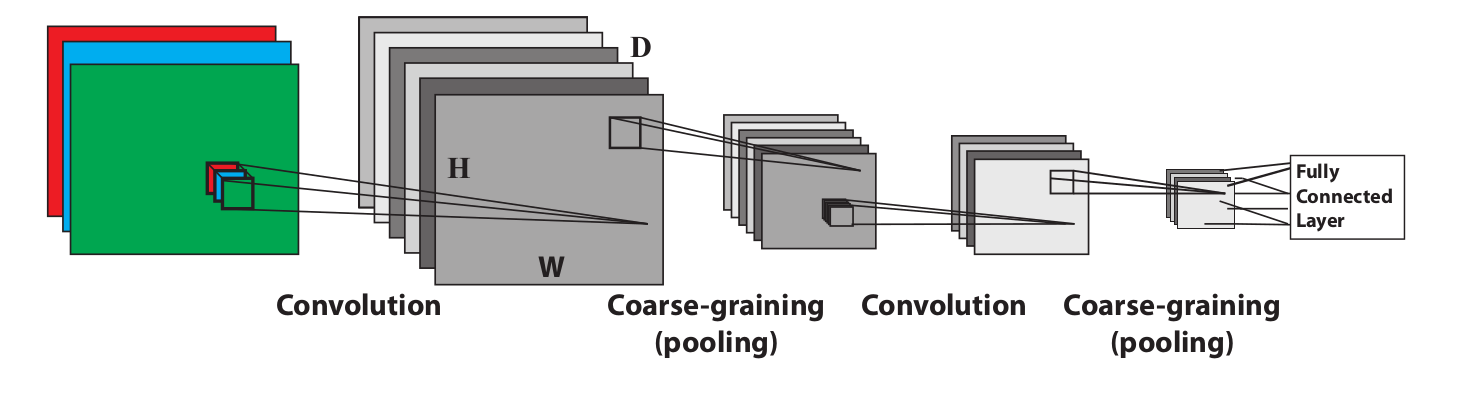
\includegraphics[width=0.8\linewidth]{gfx/cnn}
	\caption{Architecture of a CNN: \itshape The neurons in a CNN are arranged in three dimension: height $(H)$, width $(W)$, and depth $(D)$. For the input layer, the depth corresponds to the  number of channels (in this case $3$ for RGB images). Neurons in the convolutional layers calculate the convolution of the image with a local spatial filter (e.g. $3\times 3$ pixel grid, times $3$ channels for first layer) at a given location in the spatial $(W,H)$-plane. The depth $D$ of the convolutional layer corresponds to the number of filters used in the convolutional layer. Neurons at the same depth correspond to the same filter. Neurons in the convolutional layer mix inputs at different depths but preserve the spatial location. Pooling layers perform a spatial coarse graining (pooling step) at each depth to give a smaller height and width while preserving the depth. The convolutional and pooling layers are followed by a fully connected layer and classifier (not shown).}
	\label{fig:cnn}
\end{figure}

\begin{enumerate}
\item A convolution layer that computes the convolution of the input with a bank of filters\footnote{As a mathematical operation, see this practical guide to :\href{http://setosa.io/ev/image-kernels}{Image kernels}.},
\item and pooling layers that coarse-grain the input while maintaining locality and spatial structure, compare fig. \ref{fig:cnn}.
\end{enumerate}
\begin{mybox}{Pedagogical summary of CNN}
	
	The weights of a cnn are the kernel convolution operations. Each depth in the convolutional layer corresponds to one specific filter/kernel convolution applied to three $3$ input (RGB) channels. One weight/filter could correspond to a convolution that highlights all the horizontal edges, another one highlights all the vertical edges, we dont know and we dont care. The input, i.e. a face, however is a combination of features, a combination of edges, shapes etc. All of the different depths per layer will look different, will highlight different features, will be a different representation of the face, which the machine deems as important. We therefore do not pick which convolutions to apply, i.e. which features are to be highlighted, the machine does, as in a DNN. One layer in the final layer could for example be highlighted if there is a ear at a certain position, they will eventually describe one pixel. We have completely removed the spatial dimension from the $3D$ input image. At the end you have a classifier, which decides whether the resulting convolution of convolutions is a picture of Alice's face or not. Therefore, the weights (i.e. the kernel convolutions) are adjusted via (backpropagation) supervised learning as we know whether the picture corresponds to Alice or not, i.e. only the weights and dimension of the input is different but the training and prediction procedure is the same.
\end{mybox}

\subsubsection{On convolutional layers}
\label{subsubsec:cnnConvolutionalLayer}
For two-dimensional data, a layer $l$ is characterized by three numbers: height $H_l$, width $W_l$, and depth $D_l$\footnote{The depth $D_l$ is often called ’number of channels’, to distinguish it from the depth of the NN itself, i.e. the total number of layers (which can be convolutional, pooling or fully-connected), c.f. \ref{fig:cnn}.}
 The height and width correspond to the sizes of the two-dimensional spatial $(W_l, H_l)$-plane (in neurons), and the depth $D_l$ (marked by the different colours in \ref{fig:cnn})-to the number of filters in that layer. All neurons corresponding to a particular filter have the same parameters (i.e. shared weights and bias).\\
 In general, we will be concerned with local spatial filters (often called a \emph{receptive field} in analogy with neuroscience) that take as inputs a small spatial patch of the previous layer at all depths. For instance, a square filter of size $F$ is a three-dimensional array of size $F\times F\times D_{l-1}$. The convolution consists of running this filter over all locations in the spatial plane.
 \begin{example}
 	To demonstrate how this works in practice, let us consider the simple example consisting of a one-dimensional input of depth $1$, shown in fig \ref{fig:cnnExample}. In this case, a filter of size $F\times 1\times 1$ can be specified by a vector of weights $w$ of length $F$. 
 \end{example}
The stride, $S$, encodes by how many neurons we translate the filter by when performing the convolution. In addition, it is common to pad the input with $P$ zeroes (c.f. \ref{fig:cnnExample}).

\begin{figure}[h!]
	\centering
	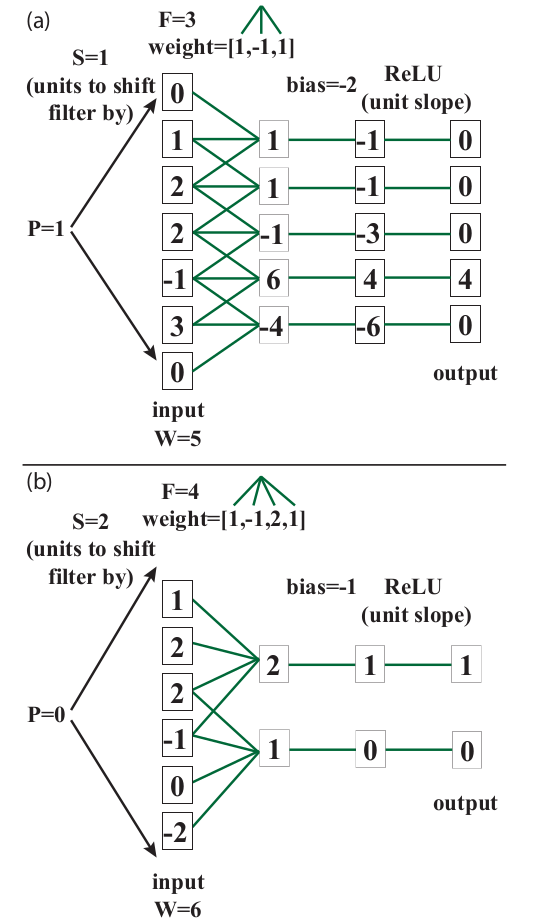
\includegraphics[width=0.4\linewidth]{gfx/cnnExample}
	\caption{Two examples to illustrate a one-dimensional convolutional layer with ReLU nonlinearity:\itshape Convolutional layer for a spatial filter of size $F$ for a one-dimensional input of width $W$ with stride $S$ and padding $P$ followed by a ReLU non-linearity.}
	\label{fig:cnnExample}
\end{figure}
For an input of width $W$, the number of neurons (outputs) in the layer is given by $(W-F+2P)/S+1$. After computing the filter, the output is passed through a non-linearity (e.g. a ReLU). In practice, one often inserts a BatchNorm layer before the non-linearity, cf. \ref{subsubsec:dnnRegularizerPracticalBatchNorm}.
\subsubsection{On pooling layers}
\label{subsubsec:cnnPooling}
The convolutional layers are interspersed with pooling layers that coarse-grain spatial information by performing a subsampling at each depth. \\
A limitation of the feature map output of convolutional layers is that they record the precise position of features in the input. This means that small movements in the position of the feature in the input image will result in a different feature map. This can happen with re-cropping, rotation, shifting, and other minor changes to the input image. A common approach to addressing this problem from signal processing is called down sampling. This is where a lower resolution version of an input signal is created that still contains the large or important structural elements, without the fine detail that may not be as useful to the task.

Down sampling can be achieved with convolutional layers by changing the stride of the convolution across the image. A more robust and common approach is to use a pooling layer.
The pooling layer operates upon each feature map separately to create a new set of the same number of pooled feature maps.
Pooling involves selecting a pooling operation, much like a filter to be applied to feature maps. The size of the pooling operation or filter is smaller than the size of the feature map; specifically, it is almost always $2×2$ pixels applied with a stride of $2$ pixels.

This means that the pooling layer will always reduce the size of each feature map by a factor of $2$, e.g. each dimension is halved, reducing the number of pixels or values in each feature map to one quarter the size. For example, a pooling layer applied to a feature map of $6×6$ ($36$ pixels) will result in an output pooled feature map of$ 3×3$ ($9$ pixels). 
\\
\\
One common pooling operation is the \emph{max pool}, another one is average pooling. In a max pool, the spatial dimensions are coarse-grained by replacing a small region (say $2\times 2$ neurons) by a single neuron whose output is the maximum value of the output in the region. This generally reduces the dimension of outputs, compare \ref{fig:cnnPooling}.
\begin{example}
	For example, if the region we pool over is $2\times 2$, then both the height and the width of the output layer will be halved. 
\end{example}
Generally, pooling operations do not reduce the depth of the convolutional layers because pooling is performed separately at each depth.
\begin{figure}[h!]
	\centering
	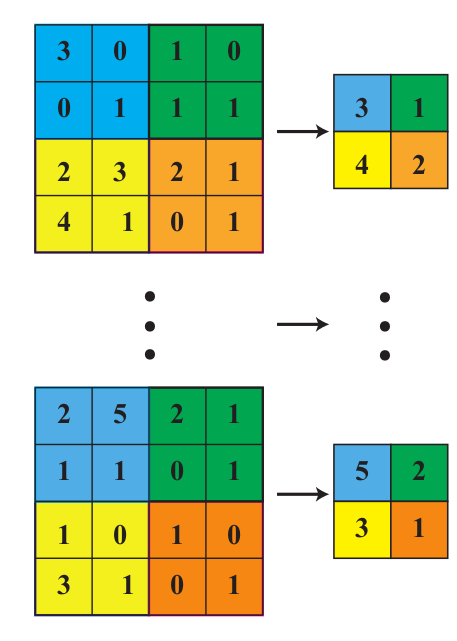
\includegraphics[width=0.7\linewidth]{gfx/cnnPooling}
	\caption{Illustration of Max Pooling: \itshape Illustration of max pooling over a $2\times 2$ region. Notice that pooling is done at each depth (vertical axis) separately. The number of outputs is halved along each dimension due to this coarse-graining.}
	\label{fig:cnnPooling}
\end{figure}
\subsubsection{Classifying layer}
In a CNN, the convolution and max-pool layers are generally followed by an all-to-all connected layer and a high-level classifier such as soft max. This allows us to train CNNs as usual using backpropagation  \ref{subsec:dnnBackpropagation}. From a backprop perspective, CNNs are almost identical to fully connected NN architectures except with tied parameters.\\
Apart from introducing additional structure, such as translational invariance and locality, this convolutional structure also has important practical and computational benefits. All neurons at a given layer represent the same filter, and hence can all be described by a single set of weights and biases. This reduces the number of free parameters by a factor of $H\times W$ at each layer.
\begin{example}
	For a layer with $D=10^2$ and $H=W=10^2$, this gives us a reduction in parameters of nearly $10^6$.
\end{example}
This allows for the training of much larger models than would otherwise be possible with fully connected layers. 









\subsection{Pre-trained CNNs and transfer learning}
\label{subsec:cnnTransferLearning}
The huge CNN models trained by industry are called: AlexNet, GoogLeNet, ResNet, InceptionNet, VGGNet, etc. The trained models have been released and are now available in standard packages such as Torch Vision library in Pytorch or the Caffe framework. These models can be used directly as a basis for fine-tuning in different supervised image recognition tasks through a process called \emph{tranfer learning}.
\begin{mybox}{Transfer learning}
	The basic idea behind transfer learning is that the filters (receptive fields) learned by the convolution layers of these networks should be informative for most image recognition based tasks, not just the ones they were originally trained for. In other words, we expect that , since images reflect the natural world, the filters learned by these CNNs should transfer over to new tasks with only slight modifications and fine-tuning.
\end{mybox}
There are three distinct ways one can take a pretrained CNN and repurpose it for a new task.
\begin{enumerate}
	\item \emph{Use CNN as fixed feature detector at top layer}:\\
	If the new dataset we want to train on is small and similar to the original dataset, we can simply use the CNN as a fixed feature detector and retrain our classifier. In other words, we remove the classifier (soft-max) layer at the top of the CNN and replace it with a new classifier (linear support vector machine (SVM) or soft-max) relevant to our supervised learning problem. In this procedure, the CNN serves as a fixed map from images to relevant features (the outputs of the top fully-connected layer right before the original classifier). This procedure prevents overfitting on small, similar datasets and is often a useful starting point for transfer learning.
	\item \emph{Use CNN as fixed feature detector at intermediate layer}:\\
	If the dataset is small and quite different from the dataset used to train the original image, the features at the top level might not be suitable for our dataset. In this case, one may want to instead use features in the middle of the CNN to train our new classifier. These features are though to be less fine-tuned and more universal (e.g. edge detectors) This is motivated by the idea that CNNs learn increasingly complex features the deeper one goes in the network (see discussion on representational learning in \ref{subsubsec:dnn2SuccessfulRepresentation}).
	
	\item \emph{Fine-tune the CNN}:\\
	If the dataset is large, in addition to replacing and retraining the classifier in the top layer, we can also fine-tune the weights of the original CNN using backpropagation. One may choose to freeze some of the weights in the CNN during the procedure or retrain all of them simultaneously.
	
\end{enumerate}
All of these procedures can be carried our easily by using packages such as Caffe or the Torch Vision library in PyTorch.\footnote{Read the \href{https://pytorch.org/tutorials/}{Pytorch tutorials} carefully if interested in transfer learning.}












\section{High-Level Concepts in Deep Neural Networks}
\label{sec:dnn2}
Here we discuss some high-level questions about the practice and performance of neural networks. 


\subsection{Organizing deep learning workflows using the bias-variance tradeoff}
\label{subsec:dnn2Workflow}
Here we present a DL workflow inspired by the bias-variance tradeoff \ref{subsubsec:biasvariancetradeoff}. This workflow is especially relevant to industrial applications where one is often trying to employ NNs to solve a particular problem.\footnote{Draws heavily from \href{https://www.youtube.com/watch?v=F1ka6a13S91}{Andrew Ng's tutorial}.}
\begin{figure}[h!]
	\centering
	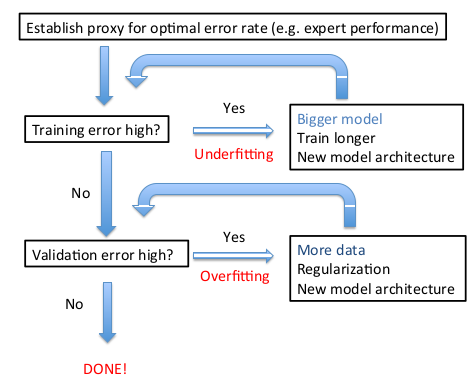
\includegraphics[width=0.7\linewidth]{gfx/WorkflowDNN}
	\caption{}
	\label{fig:dnnworkflow}
\end{figure}
The first thing we would like to do is divide the data into three parts. A training set, a validation or dev (development) set, and a test set. The test set is the data on which we want to make predictions. The dev set is a subset of the training data we use to check how well we are doing out-of-sample, after training the model on the training dataset. We use the validation error as a proxy for the test error in order to make tweaks to our model. It is crucial that we do not use any of the test data to train the algorithm. Follow the following \textbf{workflow}, compare \ref{fig:dnnworkflow}.
\begin{enumerate}
\item \emph{Estimate optimal error rate (Bayes rate).}\\
The first thing one should establish is the difficulty of the task and the best performance one can expect to achieve. No algorithm can do better than the ’signal’ in the dataset. 
\begin{example}
	It is much easier to classify objects in high-resolution images than in very blurry, low-resolution images.
\end{example}
Thus, one need to establish \textbf{a proxy or baseline for the optimal performance that can be expected from any algorithm}. In the context of Bayesian statistics, this is often called the \emph{Bayes rate}. Since we do not know this \emph{a priori}, we must get an estimate of this. For many tasks such as speech or object recognition, we can approximate this by the performance of humans on the task. For a more specialized task, we would like to ask how well experts, trained at the task, perform. This expert performance then serves as a proxy for our Bayes rate.

\item \emph{Minimize underfitting (bias) on training data set.}\\
After we have established the Bayes rate, we want to make sure that we are using a sufficiently complex model to avoid underfitting on the training dataset. In practice, this means comparing the training error rate to the Bayes rate. Since the training error does not care about generalization (variance), our model should approach the Bayes rate on the training set. If it does not, the bias of the DNN model is too large and one should try training the model longer and/or using a larger model. Finally, if none of these techniques work, it is likely that the model architecture is not well suited to the dataset, and one should modify the neural architecture in some way to better reflect the underlying structure of the data (symmetries, \emph{locality}, etc.).
\item \emph{Make sure you are not overfitting}:\\
Next, we run our algorithm on the validation or dev set. If the error is similar to the training error rate and Bayes rate, we are done. If it is not, then we are overfitting the training data. Possible solutions include, regularization and, importantly, collecting more data. Finally, if none of these work, one likely has to change the DNN architecture.
\end{enumerate}
If the validation and test sets are drawn from the same distributions, then good performance on the validation set should lead to similarly good performance on the test set. (Of course performance will typically be slightly worse on the test set because the hyperparameters were fit to the validation set.) However, sometimes the training data and test data differ in subtle ways because, for example, they are collected using slightly different methods, or because it is cheaper to collect data in one way versus another. In this case, there can be a mismatch between the training and test data. This can lead to the NN overfitting these small differences between the test and training sets, and a poor performance on the test set despite having a good performance on the validation set.
\\
One possibility to alleviate this is to make two validation or dev sets, one constructed from the training data and one constructed from the test data. The difference between the performance of the algorithm on these two validation sets quantifies the train-test mismatch. This can serve as another important diagnostic when using DNNs for supervised learning.

\subsection{Why NN are so successful: three high-level perspectives on neural networks}
\label{subsec:dnn2Successful}
\subsubsection{Neural networks as representation learning}
\label{subsubsec:dnn2SuccessfulRepresentation}
The ability of DL to learn good representations with very little hand-tuning (i.e. blackbox learning of relevant features) is very potent. Many of the other supervised learning algorithms discussed (regression-based models \ref{sec:linearRegression},\ref{sec:logisticRegression}; ensemble methods \ref{subsec:ensemblesRandomForest},\ref{subsec:ensemblesRandomForest}) perform comparably or even better than NNs but when using hand-crafted features with small-to-intermediate sized datasets.\\
The hierarchical structure of DL models is thought to be crucial to their ability to represent complex, abstract features.
\begin{example}
	Consider the use of CNNs for image classification tasks. The analysis of CNNs suggests that the lower-levels of the NNs learn elementary features, such as edge detectors, which are then combined into higher levels of networks into more abstract, higher-level features.
\end{example}
One of the interesting consequences of this line of thinking is the idea that one can train a CNN on one large dataset and the features it learns should also be useful for other supervised tasks. This results in the ability to learn important and salient features directly from the data and then transfer this knowledge to a new task\footnote{This ability to learn important, higher-level, coarse-grained features is reminiscent of ideas like RG in physics where the RG flows separate out relevant and irrelevant directions.}.

\subsubsection{Neural networks can exploit large amounts of data}
The advent of Big Data favours supervised learning methods that can fully exploit this. One important reason for the success of DNNs is that they are able to exploit the additional signal in large datasets for difficult supervised learning tasks. Fundamentally, modern DNNs are unique in that they contain million of parameters, yet can still be trained on existing hardwares. The complexity of DNNs (i.t.o. parameters) combined with their simple architecture (layer-wise connections) hit a sweet spot between expressivity (ability to represent very complicated functions) and trainability (ability to learn millions of parameters.).\\
\\
When the amount of data is small, DNNs offer no substantial benefit over conventional supervised learning algorithms (like support vector machines SVM or ensemble methods). However, large DNNs with large datasets outperform other methods by a vast amount, not having to specify parameters helps as well. It is likely that as long as a DNN is large enough, it should generalize well and not overfit.

\subsubsection{Neural networks scale up well computationally}
The architecture of NNs naturally lends itself to parallelization and the exploitation of fast but specialized processors (GPU or TPU). The layered architecture of NNs also makes it easy to use modern techniques such as automatic differentiation that make it easy to quickly deploy them. Algorithms such as SGD and the use of mini-batches make it easy to parallelize code and train much larger DNNs.

\subsection{Limitations of supervised learning with deep networks}
\label{sec:dnn2Limitations}
Often, the same or better performance on a task can be achieved by using a few hand-engineered features (or even a collection of random features). Limitations may be and are not limited to:
\begin{enumerate}
	\item \emph{Need labelled data.}
	\item \emph{Supervised NNs are extremely data intensive.}\\
	The utility of DNNs is extremely limited if data is hard to acquire or datasets are small (hundreds to a few thousand samples), especially for supervised learning where you need labels for the data.
	\item \emph{Homogeneous data.}\\
	Almost all DNNs deal with homogenoeus data of one type, very hard to design architectures that mix and match data types. Ensemble methods can do this in contrast.
	\item\emph{Many physics problems are not about prediction.}\\
	In physics, we are often not interested in solving prediction tasks such as classification. Instead, we want to learn something about the underlying distribution that generates the data. In this case, it is often difficult to cast these ideas in a supervised learning setting. While the problems are related it is possible to make good predictions with a ’wrong’ model. The model might or might not be useful for understanding the physics.	
\end{enumerate}
The use of unsupervised methods in part circumnavigates these problems.

















































\chapter{Unsupervised Learning}
\section{Dimensional Reduction and Data Visualization}
\label{sec:dimRed}
In this section, we will begin our foray into unsupervised learning by way of data visualization. Data visualization methods are important for modelling as they can be used to identify correlated or redundant features along with irrelevant features (noise) from raw or processed data. For data involving a relatively small number of features, studying pair-wise correlations (i.e. pairwise scatter plots of all features) may suffice in performing a complete analysis. This rapidly becomes impractical for datasets involving a large number of measured features (such as images). \begin{mybox}{Dimensional Reduction}
	Thus, in practice, we often have to perform \emph{dimensional reduction}, namely, project or embed the data onto a lower dimensional space, which we refer to as the \emph{latent} space.\\
	A recurrent objective of dim. red. techniques is to preserve the relative pairwise distances (or defined similarities) between data points from the original space to the latent space.
\end{mybox}
Part of the complication of dim. red. lies in the fact that low-dimensional representations of high-dimensional data necessarily incurs information loss.

\subsection{Some of the challenges of high-dimensional data}
\label{subsec:dimRedChallengesData}
\subsubsection{High-dimensional data lives near the edge of sample space}
Like one sees in statistical physics, for high-dimensional data, approximately all of the datapoints are contained only in the surface of the $D$-dimensional sphere/cube/... describing it.

\subsubsection{Real-world data vs. uniform distribution}
Fortunately, real-world data is not random or uniformly distributed.\\
In facet, real data usually lives in a much lower dimensional space than the original space in which the features are being measured. This is sometimes referred to as the \emph{blessing of non-uniformity} (in opposition to the curse of dimensionality \ref{subsubsec:performanceevalCurseDimensionality}). 
\begin{example}
	For weakly interacting particles in stat. phys., one can describe them via thermodynamic variables containing the macroscopic dynamics without having to specify the high-dimensional $N\propto 10^{23}$ amount of d.o.f. of the respective phase space dynamics of every particle in the ensemble.
\end{example}

\subsubsection{Intrinsic dimensionality and the crowding problem}
\begin{mybox}{Intrinsic dimensionality of the data}
	Qualitatively, this refers to the minimum number of dimensions (parameters) required to capture the signal in the data (to parametrize the data).  For example, if a data set is described by a sphere, then you need three parameters ($r,\vartheta,\varphi$), i.e. an intrinsic dimensionality of $3$, to parametrize the sphere $S^2 \subset \mR^3$.
\end{mybox}
\begin{mybox}{Crowding problem}
	Attempting to represent data in a space of dimensionality lower than its intrinsic dimensionality can lead to a \emph{crowding problem}. In short, because we are attempting to satisfy too many constraints (e.g. preserve all relative distances of the original space), this results in a trivial solution for the latent space where all mapped data points collapse to the centre of the map. In our example, if you collapse the sphere into two-dimensions, i.e. the circle with variable radius, the two hemispheres would be projected non-bijectively onto the circle, i.e. $\vartheta\in [0,\pi)\mapsto \vartheta=const$. Thus, you would lose a lot of information via the embedding in $\mR^2$.
\end{mybox}
To alleviate this, one needs to weaken the constraints imposed on the visualization scheme. Powerful methods such as t-distributed stochastic embedding (t-SNE) and uniform manifold approximation and projection (UMAP) have been devised to circumvent this issue in various ways.


\subsection{Principal component analysis (PCA)}
\label{subsec:dimRedPCA}
\begin{mybox}{PCA}
A ubiquitous method for dimensional reduction, data visualization and analysis is \emph{Principal Component Analysis} (PCA). The goal of PCA is to perform an orthogonal transformation of the data in order to find high-variance directions. PCA is inspired by the observation that in many cases, the relevant information in a signal is contained in the directions with largest variance. This can be seen as ’fitting’ an ellipse to the data with the major axis corresponding to the first principal component (direction of largest variance).
\end{mybox}
Such PCA-based projections often capture a lot of the large scale structure of many datasets. Even without prior physical knowledge, one can extract relevant order parameters using a simple PCA-based projection.
\subsubsection{The theory}
\label{subsubsec:dimRedPCAtheory}
Consider $N$ data points, $\{\mx_1,\dots,\mx_N\}$ that live in a $p$-dimensional feature space $\mx_i \in \mR^p$. Denote the $N\times p$ design matrix as $\mX = [\mx_1,\dots,\mx_N]^T$ whose rows are the data points and columns correspond to different features, compare \ref{subsec:recipeML}. The $p\times p$ (symmetric) covariance matrix is therefore 
\be 
\label{eq:dimRedPCAcovMatrix}
\mS(\mX) = \frac{1}{N-1} \mX^T \mX.
\ee 
notice that the $j$-th diagonal entry of $\mS(\mX)$ corresponds to the variance of the $j$-th feature and $\mS(\mX)_{ij}$ measures the covariance (i.e. connect correlation in the language of physics) between feature $i$ and feature $j$.\\
Via singular value decomposition (SVD), one finds
\be 
\mS(\mX) = \mathbf{V} \left(\frac{\mathbf{S}^2}{N-1}\right) \mathbf{V}^T \equiv \mathbf{V}\mathbf{Λ} \mathbf{V}^T,
\ee 
where $\mathbf{V}$ contains (as its columns) the right singular vectors of $\mX$, and $\mathbf{Λ}$ is a diagonal matrix with eigenvalues $\lambda_i =s^2_i/(N-1)$ ($s_i$ are the singular values) in the decreasing order along the diagonal (i.e. eigendecomposition). It is clear that the right singular vectors of $\mX$ (i.e. the columns of $\mathbf{V}$) are principal directions of $\mS(\mX)$, and the singular values of $\mX$ are related to the eigenvalues of the covariance matrix $\Sigma(\mX)$ via $\lambda_i$. To reduce the dimensionality of data from $p$ to $\tilde{p}<p$, we first construct the $p\times \tilde{p}$ projection matrix $\mathbf{V}_{\tilde{p}}$ by selecting the singular components with the $\tilde{p}$ largest singular values. The projection of the data from $p$ to $\tilde{p}$ is simply $\tilde{\mathbf{Y}}=\mX \mathbf{V}_{\tilde{p}}$. \\
The singular vector with the largest singular value (i.e. the largest variance) is referred to as the first principal component; the singular vector with the second largest singular value as the second principal component, and so on. An important quantity is the ratio $\lambda_i/\sum_{i=1}^p \lambda_i$ which is referred as the \emph{percentage of the explained variance contained in a principal component}.\\
It is common in data visualization to present the data projected on the first few principal components. This is valid as long as a large part of the variance is explained in those components. Low values of explained variance may imply that the intrinsic dimensionality of the data is high or simply that it cannot be captured by a linear representation.

\subsection{Multidimensional scaling}
\label{subsec:dimRedMDS}
\begin{mybox}{MDS}
	Multidimensional scaling (MDS) is a non-linear dimensional reduction technique which preserves the pairwise distance or dissimilarity $d_{ij}$ between data points. There are two types of MDS, metric and non-metric.
\end{mybox}
\subsubsection{Metric MDS}
In metric MDS, the distance is computed under a pre-defined metric and the latent coordinates $\tilde{\mathbf{Y}}$ are obtained by minimizing the difference between the distance measured in the original space ($d_{ij}(\mx)$) and that in the latent space ($d_{ij}(\mathbf{Y})$):
\be 
\label{eq:dimRedMDS}
\tilde{\mathbf{Y}} = \arg \min_{\mathbf{Y}} \sum_{i<j} w_{ij} \abs{d_{ij} (\mX)-d_{ij}(\mathbf{Y})},
\ee 
where $w_{ij}\geq 0$ are weight values. The weight matrix $w_{ij}$ is a set of free parameters that specify the level of confidence (or precision) in the value of $d_{ij}(\mX)$. If Euclidean metric is used, MDS gives the same result as PCA and is usually referred to as classical scaling. Thus MDS is often considered as a generalization of PCA.

\subsubsection{Non-metric MDS}
In non-metric MDS, $d_{ij}$ can be any distance matrix. The objective function is then to preserve the ordination in the data, i.e. if $d_{12}(\mX) < d_{13}(\mX)$  in the original space, then in the latent space we should have $d_{12}(\mathbf{Y})< d_{13}(\mathbf{Y})$.

\subsubsection{General comment}
Both MDS and PCA can be implemented using standard Python packages such as Scikit. They are often among the first data visualization techniques one resorts to.

\subsection{t-SNE}
\label{subsec:dimRedTSNE}
It is often desirable to preserve local structures in high-dimensional datasets. However, when dealing with datasets having clusters delimitated by complicated surfaces or datasets with a large number of clusters, preserving local structures becomes difficult using linear techniques such as PCA\footnote{Non-linear techniques such as non-classical MDS, self-organizing map, Isomap and Locally Linear Embedding preserve local structures but fail to capture structures at the larger scale such as the clusters in which the data is organized.}.
\marginpar{Non-parametric here means that it does not explicitly parametrize feature extraction required to compute the embedding coordinates. Thus it cannot be applied to find the coordinate of new data points.}
\begin{mybox}{t-SNE}
	Recently, $t$-stochastic neighbour embedding ($t$-SNE) has emerged as one of the go-to methods for visualizing high-dimensional data. $t$-SNE is a non-parametric method that constructs non-linear embeddings. Each high-dimensional training point is mapped to low-dimensional embedding coordinates, which are optimized in a way to preserve the local structure in the data.
\end{mybox}
\subsubsection{The theory}
The idea of stochastic neighbour embedding is to associate a probability distribution to the neighbourhood of each data (note $x\in \mR^p$, $p$ is the number of features):
\be 
p_{i|j} = \frac{\exp(-\norm{x_i-x_j}^2/2 \sigma^2_i)}{\sum_{k\neq i} \exp(-\norm{x_i-x_k}^2/2 \sigma^2_i)},
\ee 
where $p_{i|j }$ can be interpreted as the likelihood that $x_j$ is $x_i$'s neighbour (thus we take $p_{i|i}=0$). $\sigma_i$ are free bandwidth parameters that are usually determined by fixing the local entropy $H(p_i)$ of each data point:
\be 
H(p_i) \equiv -\sum_j p_{j|i}\log_2 p_{j|i}.
\ee 
The local entropy is then set to equal a constant across \emph{all data points} $\Sigma = 2^{H(p_i)}$, where $\Sigma$ is called the \emph{perplexity}. The perplexity constraint determines $\sigma_i \forall i$ and implies that points in regions of high-density will have smaller $\sigma_i$.\\
\\
Using Gaussian likelihoods in $p_{i|j}$ implies that only points that are nearby $x_i$ contribute to its probability distribution. This ensures that the similarity for nearby points is well represented but neglects the contributions of points far away. To alleviate this, we define a symmetrized distribution $p_{ij} \equiv (p_{i|j}+p_{j|i})/(2N)$. This \emph{guarantees} that $\sum_j p_{ij} >1/(2N)$ for all data points $x_i$, resulting in each data point $x_i$ making a significant contribution to the cost function to be defined below.
\begin{mybox}{tSNE}
	$t$-SNE constructs a \emph{similar} probability distribution $q_{ij}$ in a low dimensional latent space (with coordinates $Y=\{y_i\}, y_i \in \mR^{p^\prime}$, where $p^\prime <p$ is the dimension of the latent space):
	\be 
	\label{eq:dimRedTSNEprobdistr}
	q_{ij} = \frac{(1+\norm{y_i-y_j}^2)^{-1}}{\sum_{k\neq i} (1+\norm{y_i-y_k}^2)^{-1}}.
	\ee 
	The crucial point to note is that $q_{ij}$ is chosen to be a longtail distribution. This preserves short distance information (relative neighbourhoods) while strongly repelling two points that are far apart in the original space.\\
	In order to find the latent space coordinates $y_i$, $t$-SNE minimizes the Kullback-Leibler divergence between $q_{ij}$ and $p_{ij}$:
	\be 
	\label{eq:dimRedTSNECostfct}
	\mC(Y) = D_{KL} (p||q) \equiv \sum_{ij} p_{ij} \log\left(\frac{p_{ij}}{q_{ij}}\right).
	\ee 
	This minimization is done via GD (see \ref{sec:gd}).
\end{mybox}
Computing the gradient of \ref{eq:dimRedTSNECostfct}, we can see what the embedding cost-function $\mC$ is capturing
\begin{align}
	\label{eq:dimRedTSNEForce}
	\partial_{y_i} \mC&=\sum_{j\neq i} 4 p_{ij} q_{ij} Z_i(y_i-y_j) - \sum_{j\neq i} 4 q^2_{ij} Z_i(y_i-y_j)\nonumber \\
	&= F_{\text{attractive,}i} -F_{\text{repulsive,}i},
\end{align}
where $Z_i=1/(\sum_{k\neq i} (1+\norm{y_k-y_i}^2)^{-1})$. Notice that $F_{\text{attractive,}i}$ induces a significant attractive force only between points that are nearby point $i$ in the \emph{original space} since it involves the $p_{ij}$ term. Finding the embedding coordinates $y_i$ is thus equivalent to finding the equilibrium configuration of particles interacting through forces, compare \ref{eq:dimRedTSNEForce}.\\
\\
The $t$-SNE visualization cleanly separates all the clusters while certain clusters blend together in PCA for example. This is a direct consequence of the fact that $t$-SNE keeps nearby points close together while repelling points that are far apart, compare \ref{eq:dimRedTSNEForce}.

\subsubsection{Important properties of $t$-SNE}
\begin{enumerate}
\item $t$-SNE can rotate data:\\
The KL divergence is invariant under rotations in the latent space, i.e. $t$-SNE plots that are rotations of each other should be considered equivalent.
\item $t$-SNE results are stochastic.\\
In applying GD, the solution of different $t$-SNE runs depends on the initial seed and results in different outcomes.
\item \emph{$t$-SNE generally preserves short distance information}.\\
As a rule of thumb, one should expect that nearby points on the $t$-SNE map are also closeby in the original space, i.e. $t$-SNE tends to preserve ordination (but not actual distances).
\item \emph{Scales are deformed in $t$-SNE}.\\
Since a scale-free distribution is used in the latent space, one should not put too much emphasis on the meaning of the size of any clusters observed in the latent space.
\item \emph{$t$-SNE is computationally intensive}:\\
$\mO(N^2)$.
\end{enumerate}





\section{Clustering}
\label{sec:cluster}
This section is also concerned with unsupervised learning methods.\\
Unsupervised learning is concerned with discovering structure in unlabelled data (for instance learning local structures for data visualization \ref{sec:dimRed}). The lack of labels make unsupervised learning much more difficult and subtle than its supervised counterpart. What is somewhat surprising is that even without labels it is still possible to uncover and exploit the hidden structure in the data. Perhaps, the simplest example of unsupervised learning is clustering.
\begin{mybox}{Clustering}
 The aim of clustering is to group unlabelled data into clusters according to some similarity or distance measure. Informally, a cluster is thought of as a set of points sharing some pattern or structure.\\
 Clustering finds many applications throughout data mining, data compression and signal processing. Clustering can be used to identify coarse features or high level structures in an unlabelled dataset.
\end{mybox}
The field of clustering is vast and there exists a flurry of clustering methods suited for different purposes. Some common considerations one has to take into account when choosing a particular method is the distribution of the clusters (overlapping/noisy clusters vs. well-separated clusters), the geometry of the data (flat vs. non-flat), the cluster size distribution (multiple sizes vs. uniform sizes), the dimensionality of the data (low vs. high dimensional) and the computational efficiency of the desired method (small vs. large dataset).


\subsection{Practical clustering methods}
\label{subsec:clusterPractical}
Throughout this section we focus on the Euclidean distance as a similarity measure.

\subsubsection{$K$-means}
\label{subsubsec:clusterPracticalKmeans}

Consider a set of $N$ \emph{unlabelled} observations $\{\mx_n\}^N_{n=1}$ where $\mx_n\in \mR^p$ and where $p$ is the number of features. Also consider a set of $K$ cluster centres called the cluster \emph{means}: $\{\mathbf{μ}_k\}^K_{k=1}$, with $\mathbf{μ}_k\in \mR^p$, which we'll compute ’empirically’ in the clustering procedure. The cluster means can be thought of as the representatives of each cluster, to which data points are assigned. 
\begin{mybox}{$K$-means set-up}
	$K$-means clustering can be formulated as follows: given a fixed integer $K$, find the cluster means $\{\mathbf{μ}\}$ and the data point assignments in order to minimize the following objective function
	\be
	\label{eq:clusterPracticalKmeansCostfct}
	\mC(\{x,\mathbf{μ}\}) = \sum_{k=1}^K \sum_{n=1}^N r_{nk} ( \mx_n - \mathbf{μ}_k)^2,
	\ee
	where $r_{nk} \in \{0,1\}$ is a binary variable called the \emph{assignment}. The assignment $r_{nk}$ is $1$ if $x_n$ is assigned to cluster $k$ and $0$ otherwise. Notice that $\sum_k r_{nk}=1 \forall n$ and $\sum_n r_{nk}\equiv N_k$, where $N_k$ is the number of points assigned to cluster $k$. The minimization of this objective function can be understood as trying to find the best cluster means such that the variance within each cluster is minimized.
\end{mybox}
In physical terms, $\mC$ is equivalent to the sum of the moments of inertia of every cluster. The cluster means $\mathbf{μ}_k$ correspond to the centres of mass of their respective cluster.
\begin{mybox}{$K$-means algorithm}
	The $K$-means algorithm alternates between two steps:
	\begin{enumerate}
		\item \emph{Expectation}: Given a set of assignments $\{r_{nk}\}$, minimize $\mC$ w.r.t. $\mathbf{μ}_k$. Taking a simple derivative and setting it to zero yields the following update rule:
		\be 
		\mathbf{μ}_k = \frac{1}{N_k} \sum_n r_{nk} \mx_n.
		\ee 
		\item \emph{Maximization}: Given a set of cluster means $\{\mathbf{μ}_k\}$, find the assignments $\{r_{nk} \}$ which minimize $\mC$. Clearly, this is achieved by assigning each data point to their nearest cluster-mean:
		\be
		r_{nk} = \left\{ \begin{array}{ll}
		1 & \text{if } k=\arg \min_{k^\prime} (\mx_n-\mathbf{μ}_{k^\prime})^2 \\
		0& \text{otherwise}.
		\end{array}\right\}
		\ee 
	\end{enumerate}
Practically, the algorithm should terminate when the change in the objective function from one iteration to another becomes smaller than a pre-specified threshold.
\end{mybox}
A nice property of the $K$-means algorithm is that it is guaranteed to converge.\footnote{To see this, one can verify explicitly (by taking second-order derivatives) that the expectation and assignment step respectively always decrease $\mC$. Thus, since $\mC$ is bounded from below, the two-step iteration of $K$-means \emph{always} converges to a local maximum of $\mC$. Since $\mC$ is generally a non-convex function, in practice one usually needs to run the algorithm with different initial random cluster centre initializations and post-select the best local minimum.} The complexity is $\mO(KN)$ per iteration and is thus scalable to very large datasets.\\
A common drawback of $K$-means is the following:\\
If the true clusters have very different variances (spreads), $K$-means can lead to spurious results since the underlying assumption is that the latent model has uniform variances.\\
\\
We can measure the performance of $K$-means by thinking about the distortion- the square distance of each point from the centroid defining the cluster. This is the objective function that K-means tries to optimize.

\subsubsection{Hierarchical clustering: Agglomerative methods}
\label{subsubsec:clusterPracticalHierarchical}
Agglomerative clustering is a bottom up approach that starts from small initial clusters which are then progressively merged to form larger clusters.
\begin{figure}[h!]
	\centering
	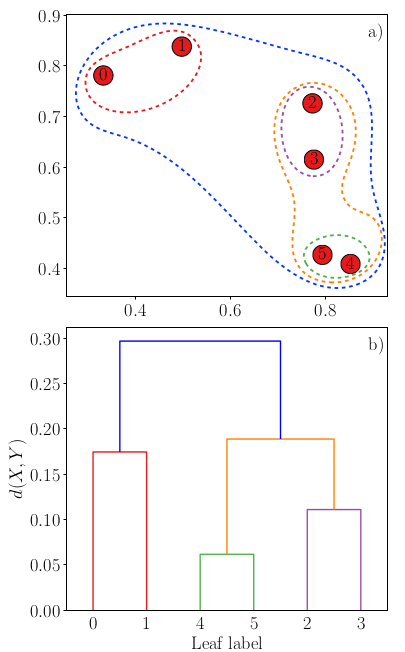
\includegraphics[width=0.4\linewidth]{gfx/HierarchicalCLustering}
	\caption{\itshape The merging process generates a hierarchy of clusters that can be visualized in the form of a dendrogram.}
	\label{fig:hierarchicalclustering}
\end{figure}
This hierarchy \ref{fig:hierarchicalclustering} can be useful to analyze the relation between clusters and the subcomponents of individual clusters. Agglomerative methods are usually specified by defining a distance measure between clusters. Different choices of distance result in different clustering algorithms. At each step, the two clusters that are the closest w.r.t. the distance measure are merged until a single cluster is left.

\begin{mybox}{Agglomerative clustering algorithm}
	\begin{enumerate}
		\item Initialize each point to its own cluster.
		\item Given a set of $K$ clusters $X_1,X_2,\dots,X_K$, merge clusters until one cluster is left ($K=1$):
		\begin{enumerate}
			\item Find the closest pair of clusters $(X_i,X_j)$:
			\bse 
			(i,j)=\arg \min_{i^\prime,j^\prime} d(X_{i^\prime},X_{j^\prime} )
			\ese 
			\item Merge the pair. Update. $K\leftarrow K-1$.
		\end{enumerate}
	\end{enumerate}
\end{mybox}
The most popular distances used in agglomerative methods, often called \emph{linkage methods}
\begin{enumerate}
	\item Single-linkage: the distance between clusters $i$ and $j$ is defined as the minimum distance between two elements of the different clusters
\be
\label{eq:ClusterPracticalHierarchicalSinglelinkage}
d(X_i,X_j) = \min_{\mx_i \in X_i,\mx_j \in X_j} \norm{\mx_i-\mx_j}_2. 
\ee 
\item Complete linkage: the distance between clusters $i$ and $j$ is defined as the maximum distance between two elements of the different clusters
\be 
\label{eq:ClusterPracticalHierarchicalCompleteLinkage}
d(X_i,X_j) = \max_{\mx_i \in X_i,\mx_j\in X_j} \norm{\mx_i-\mx_j}_2.
\ee 
\item Average linkage: average distance between points of different clusters
\be 
\label{eq:ClusterPracticalHierarchicalAverageLinkage}
d(X_i,X_j) = \frac{1}{\abs{X_i}\cdot \abs{X_j}} \sum_{\mx_i \in X_i,\mx_j\in X_j} \norm{\mx_i-\mx_j}_2.
\ee 
\item Ward's linkage: This distance measure is analogous to the $K$-means method as it seeks to minimize the total inertia. The distance measure is the ’error squared’ before and after merging which simplifies to
\be 
\label{eq:ClusterPracticalHierarchicalWardsLinkage}
d(X_i,X_j) = \frac{\abs{X_i} \abs{X_j}}{\abs{X_i \cup X_j}} (\mathbf{μ}_i-\mathbf{μ}_j)^2, 
\ee 
where $\mathbf{μ}_j$ is the centre of cluster $j$.
\end{enumerate}
A common drawback of hierarchical methods is that they do not scale well: At every step, a distance matrix between all clusters must be updated/computed. This leads to a complexity of $\mO(N^2)$, i.e. the method is suitable for small to medium-size datasets.

\subsubsection{Density-based (DB) clustering}
\label{subsubsec:clusterPracticalDBSCAN}
Density clustering makes the intuitive assumption that clusters are defined by regions of space with higher density of data points. Data points that constitute noise or that are outliers are expected to form regions of low density. The method is also suitable for large-scale applications.\\
The core assumption of DB clustering is that a \emph{relative} local density estimation of the data is possible. In other words, it is possible to order points according to their densities. Density estimates are usually accurate for low-dimensional data but become unreliable for high-dimensional data due to large sampling noise.\\
\\
	Consider a set of $N$ data points $X\equiv \{\mx_n\}^N_{n=1}$. Define the $\epsilon$-neighbourhood of point $\mx_n$ 
\be 
N_{\epsilon} (\mx_n) = \{\mx \in X| \md(\mx,\mx_n) < \epsilon \}.
\ee 
$N_{\epsilon}(\mx_n)$ are the data points that are at a distance smaller than $\epsilon$ from $\mx_n$, $\md(\cdot,\cdot)$ is the Euclidean metric. $N_{\epsilon}(\mx_n)$ can be seen as a crude estimate of local density. $\mx_n$ is considered to be a \emph{core-point} if at least \textbf{minPts} are in its $\epsilon$-neighbourhood. \textbf{minPts} is a free parameter of the algorithm that sets the scale of the size of the smallest cluster one should expect. Finally, a point $\mx_i$ is said to be \emph{density-reachable} if it is in the $\epsilon$-neighbourhood of a \emph{core-point}.
\begin{mybox}{DBSCAN algorithm}
\begin{enumerate}
	\item[$\rightarrow$] Until all points in $X$ have been visited; \textbf{do}
	\begin{enumerate}
		\item Pick a point $\mx_i$ that has not been visited
		\item Mark $\mx_i$ as a visited point
		\item If $\mx_i$ is a core point; \textbf{then}
		\begin{enumerate}
			\item Find the set $C$ of all points that are \emph{density reachable} from $\mx_i$.
			\item $C$ now forms a cluster. Mark all points within that cluster as being visited.
		\end{enumerate}
	\end{enumerate}
	\item[$\rightarrow$] Return the cluster assignments $C_1,\dots,C_k$, with $k$ the number of clusters. Points that have not been assigned to a cluster are considered noise or outliers.
\end{enumerate}
\end{mybox}
DBSCAN is very efficient with a $\mO(N\log N)$.

\subsection{Clustering and Latent Variables via the Gaussian Mixture Models}
\label{subsec:clusterConcepts}
Here we collect important concepts of unsupervised learning and showcase them via GMM.
\subsubsection{Important concepts in unsupervised learning}
\label{subsubsec:clusterConceptsCollection}

\begin{mybox}{Important concepts in unsupervised learning}
	\label{subsubsec:clusterConceptsCollectionImportant}
\begin{enumerate}
\item It is often useful to think of the visible correlations between features in the data as resulting from hidden or latent variables.
\item We will often posit a generative model that encodes the structure we think exists in the data and then find the parameters that maximize the likelihood of the observed data.
\item Often we will not be able to directly estimate the MLE, and will have to instead look for a computationally efficient way to find a local minimum of the likelihood.
\end{enumerate}
\end{mybox}
A central concept in many unsupervised learning techniques is the idea of a latent or hidden variable. Even though latent variables are not directly observable, they still influence the visible structure of the data. 
\begin{example}
In the context of clustering we can think of the cluster identity of each datapoint (i.e. which cluster does a datapoint belong to) as a latent variable.
\end{example}
The latent variables in our data (cluster identity) are a way of representing and abstracting the correlations between datapoints.\\

\begin{mybox}{Clustering}
We can think of clustering as an algorithm to learn the most probable value of a latent variable (cluster identity) associated with each datapoint.
\end{mybox}
 Calculating these latent variables requires additional assumptions about the structure of our dataset. Like all unsupervised learning algorithms, in clustering we must make an assumption about the underlying probability distribution from which the data was generated. Our model for how the data is generated is called the \emph{generative model}. In clustering, we assume that data points are assigned a cluster, with each cluster characterized by some \emph{cluster-specific} probability distribution  (e.g. Gaussian with some mean and variance that charaterizes the cluster). We then specify a procedure for finding the value of the latent variable. This is often done by choosing the values of the latent variable that minimize some cost function.\\
 \\
 One common choice for a class of cost functions for many unsupervised learning problems is MLE \ref{subsubsec:bayesEstMLE}. In MLE, we choose the values of the latent variables that maximize the likelihood of the observed data under our generative model (i.e. maximize the probability of getting the observed dataset under our generative model).
 
 
 
 
 
 
 
 \begin{mybox}{Cluster validation}
 	\label{subsubsec:clusterConceptsValidation}
 	\emph{Cluster validation} describes the procedure of verifying whether the obtained labels are ’valid’, which is usually done by visual inspection. That is, the data is represented in a low-dimensional space and the cluster labels obtained are visually inspected to make sure that different labels organize into distinct ’blobs’. This is particularly difficult for high-dimensional data, cf. \ref{subsec:clusterHighD}.
 \end{mybox}
 
 
 
 
\subsubsection{Concepts visualized via the Gaussian Mixture Model (GMM)}
\label{subsubsec:clusterConceptsGMM}
Gaussian Mixture Models are a generative model often used in the context of clustering. In GMM, points are drawn from one of $K$ Gaussians, each with its own mean $\mathbf{μ}_k$ and covariance matrix $\Sigma_k$,
\be 
\label{eq:clusterGMMGaussian}
\mathcal{N}(\mx |\mathbf{μ},\mS) \sim \exp \left[-\half (\mx -\mathbf{μ}) \mS^{-1} (\mx-\mathbf{μ})^T\right].
\ee 
Let us denote the probability that a point is drawn from mixture $k$ by $\pi_k$. Then the probability of generating a point $\mx$ in a GMM is given by
\bse 
p(\mx | \{\mm_k,\mS_k,\pi_k \})= \sum_{k=1}^K \mathcal{N}(\mx |\mm_k,\mS_k) \pi_k.
\ese 
Given a dataset $\mX=\{\mx_1,\dots,\mx_N\}$, we can write the likelihood of the dataset as
\bse 
p(\mX | \{\mm_k,\mS_k,\pi_k\}) = \prod_{i=1}^N p(\mx_i| \{\mm_k,\mS_k,\pi_k \} ).
\ese 
For future reference, let us denote the set of parameters (of $K$ Gaussians in the model) $\{\mm_k,\mS_k,\pi_k\}$ by $\mt$.\\
\\
We will now go through this model exemplifying the important concepts lined out in \ref{subsubsec:clusterConceptsCollectionImportant} in the exact same steps to give an example of these.
\begin{enumerate} 
	\item 
To see how we can use GMM and MLE to perform clustering, we introduce discrete binary $K$-dimensional latent variables $\mathbf{z}$ for each data point $\mx$ whose $k$-th component is $1$ if point $\mx$ was generated from the $k$-th Gaussian and zero otherwise (i.e. one-hot variables).
For instance, if we were considering a Gaussian mixture with $K=3$, we would have three possible values for $\mathbf{z}\equiv (z_1,z_2,z_3): (1,0,0),(0,1,0)$ and $(0,0,1)$. We cannot directly observe the variable $\mathbf{z}$. It is a latent variable that encodes the cluster identity of point $\mx$. Let us also denote all the $N$ latent variables corresponding to a dataset $\mX$ by $\mathbf{Z}$.
\item 
Viewing the GMM as a generative model, we can write the probability $p(\mx |\mathbf{z})$ of observing a data point $\mx$ given $\mathbf{z}$ as\footnote{Note that the notation with $;$ is something we have seen in \ref{eq:infoMutualInfo}, it describes a conditional dependence and makes a distinction between data and parameters.}
\bse 
p(\mx | \mathbf{z}; \{ \mm_k,\mS_k\} ) = \prod_{k=1}^K \mathcal{N}(\mx |\mm_k,\mS_k)^{z_k}
\ese 
as well as the probability of observing a given value of latent variable
\bse 
p(\mathbf{z}| \{\pi_k\}) = \prod_{k=1}^K \pi^{z_k}_k.
\ese 
Using Bayes' rule \ref{eq:bayesrule}, we can write the joint probability of a clustering assignment $\mathbf{z}$ and a data point $\mx$ given the GMM parameter as
\bse 
p(\mx ,\mathbf{z};\mt) = p(\mx| \mathbf{z}; \{\mm_k,\mS_k\} ) p(\mathbf{z}|\{\pi_k\}).
\ese 
Using Bayes' again we find the conditional probability of the data point $\mx$ being in the $k$-th cluster, $\gamma(z_k)$, given model parameters $ \theta$ as 
\be 
\label{eq:clusterConceptsGMMresponsibility}
\gamma(z_k)\equiv p(z_k=1 | \mx;\theta)= \frac{\pi_k \mathcal{N}(\mx|\mu_k,\Sigma_k)}{\sum_{j=1}^K \pi_j \mathcal{N}(\mx |\mu_j,\Sigma_j)}.
\ee 
The $\gamma(z_k)$ are often referred to as the \emph{responsibility} that mixture $k$ takes for explaining $\mx$. Just like in our discussion of soft-max classifiers, this can be made into a ’hard-assignment’ by assigning each point to the cluster with the largest probability: $\arg \max_k \gamma(z_k)$ over the responsibilities.\\
\\
The complication is of course that we do not know the parameters $\mt$ of the underlying GMM but instead must also learn them from the dataset $\mX$. Ideally we would do this by choosing the parameters that maximize the likelihood of the data
\bse 
\hat{\mt} = \arg \max_{\mt} \log p(\mX|\mt).
\ese 
Once we know the MLEs $\hat{\mt}$, we could use \ref{eq:clusterConceptsGMMresponsibility} to calculate the optimal hard cluster assignment $\arg \max_k \hat{\gamma}(z_k)$ where $\hat{\gamma}(z_k) =p(z_k=1|\mx;\hat{\mt})$.

\item It is almost impossible to find the global maximum of the likelihood function. Instead, we must settle for a local maximum. One approach to finding a local maximum of the likelihood is to use a method like SGD \ref{subsubsec:gdSGD} on the negative log-likelihood (i.e. the cost function \ref{eq:bayesErrorFct}), or expectation minimization \ref{subsec:varMFTEM}.
\end{enumerate}


\subsection{Clustering in high dimensions}
\label{subsec:clusterHighD}
One major problem that is aggravated in high-dimensions is the generic accumulation of noise due to random measurement error for each feature. This in turn leads to increased errors for pairwise similarity and distance measures and thus tends to ’blur’ distances between data points.\\
\\
In order to perform clustering on high-dimensional data, it is often useful to denoise the data before proceeding using a standard clustering method such as $K$-means \ref{subsubsec:clusterPracticalKmeans}. 
For example, PCA \ref{subsec:dimRedPCA} can be used to denoise the data by projecting the original $N$ dimensions onto $n < N$ (i.e. $20n\approx N$) with the largest principal components. The resulting features can then be used to construct a Euclidean distance matrix, which in turn can be used by $t$-SNE \ref{subsec:dimRedTSNE} to compute the embedding that is presented. Using $t$-SNE directly on original data leads to a ’blurring’ of the clusters.\\
However, simple feature selection or feature denoising (using PCA for instance) can sometimes be insufficient for learning clusters due to the presence of large variations in the signal and noise of the features that are relevant for identifying the underlying clusters.

\subsubsection{Cluster validation in high dimensions}
For high-dimensional data, cluster validation \ref{subsubsec:clusterConceptsValidation} is done by performing dimensional reduction \ref{sec:dimRed}. However, this can lead to the appearance of spurious clusters since dimensional reduction inevitably loses information about the original data, i.e. use methods with care.\\
Perhaps one of the most intuitive ways of defining a good clustering is by measuring how well the clusters generalizes. Clustering methods based on leveraging powerful classifiers to measure the generalization errors of the \href{https://pypi.org/project/hal-x/}{cluster} could be promising.


\subsection{Practical considerations of clustering methods - when do we use which method ?}
When tuning a clustering method it is important to understand what the implicit assumption of the clustering method are. For instance, methods based on density (local information), will typically fare well at clustering topological datasets since points are connected from neighbour to neighbour. At the same time, methods based on long-distance information ($𝐾$-means for instance), will typically perform poorly in such instances. Density-based methods will, however, have more difficulty at dealing with datasets with large fluctuations in the density distribution of the dataset (3rd row). Another drawback of density based methods is that they do not generalize well to high-dimensional space due to large sampling noise in the density estimates.








\section{Variational Methods and Mean-Field Theory (MFT)}
\label{sec:varMFT}
\subsection{Variational methods introduction}
\label{subsec:varMFTconcept}
A common thread in many unsupervised learning tasks is accurately representing the underlying probability distribution from which a dataset is drawn. When dealing with complicated probability distributions, it is often much easier to learn the \emph{relative weights} of different states or data points (ratio of probabilities), than \emph{absolute} probabilities. 
\begin{example}
	This is the case for statistical physics, where the whole partition function drops out in ratios of cumulants. 
\end{example}
One approach to solve for partition functons is to use Monte-Carlo based methods to draw samples from the underlying distribution (this can be done knowing only the relative probabilities) and then use these samples to numerically estimate the partition function. This is the philosophy behind powerful methods such as Markov Chain Monte Carlo (MCMC).\\
\\
An alternative approach are via variational methods, an example of which is Mean-Field Theory in statistical physics. We use this in the following to explore the concepts of Variational Methods and visualize them on the Ising model.



\subsection{Variational mean-field theory via Ising model}

\subsubsection{Important concepts of MFT}
\label{subsubsec:varMFTconcepts}
\begin{mybox}{Idea variational method}
The alternative approach is to approximate the probability distribution $p(\mx)$ and partition function using a \emph{variational distribution} $q(\mx;\theta_q)$ whose partition function we can calculate exactly. The variational parameters $\theta_q$ are chosen to make the variational distribution as close to the true distribution as possible, this is where the name ’variational distribution’ comes from, because we vary the parameters $\theta_q$.\\
MFT can be naturally understood as a procedure for approximating the true distribution of the system by a factorized distribution.
\end{mybox}
Variational MFT is a systematic way for constructing such an approximate distribution $q(\mx;\theta_q)$.\\
Even though MFT is not exact, it can often yield qualitatively and even quantitatively precise predictions (especially in high dimensions). The discrepancy between the true physics and MFT predictions stems from he fact that the variational distribution $q$ we chose cannot capture correlations. These correlations become less and less important in higher dimensions and the MFT ansatz becomes more accurate.\\
We emphasize that the failure of any particular variational ansatz does not compromise the usefulness of the approach. In some cases, one can consider changing the variational ansatz to improve the predictive properties of the corresponding variational MFT.
\subsubsection{On the example of the Ising model}
\label{subsubsec:varMFTising}
Here we discuss the ideas given in \ref{subsubsec:varMFTconcepts} on the example of the Ising model.\\
The probability of finding the Ising system in a given spin configuration at temperature $\beta^{-1}$ is given by
\bse 
p(\mathbf{s} |\beta,\mathbf{J}) = \frac{1}{Z_p(\mathbf{J})} e^{-\beta E(\mathbf{s},\mathbf{J}) }.
\ese 
Even though the true probability distribution $p(\mathbf{s}|\beta,\mathbf{J})$ may be a very complicated object, we can still make progress by approximating $p(\mathbf{s}|\beta,\mathbf{J})$ by a \emph{variational distribution}
$q(\mathbf{s},\mt)$ which captures the essential features of interest, with $\mt$ some parameters that define our variational ansatz.\\
The main idea is to choose parameters that minimize the difference between the variational free-energy $F_q(\mathbf{J},\mt)$ and the true free-energy $F_p(\mathbf{J}|\beta)$. This is
\bse 
F_q(\mathbf{J},\mt) = F_p(\mathbf{J},\beta) + D_{KL}(q||p),
\ese 
with the KL-divergence \ref{eq:infoKLdivergence}. Its properties show us that the variational free-energy is always larger than the true free energy $F_q (\mathbf{J},\mt) \geq F_p(\mathbf{J})$,with equality if and only if $q=p$ (the latter inequality is known as Gibbs inequality). They also show us that finding the best variational free-energy is equivalent to minimizing the KL divergence.
\\
\\
One starts the MFT by making an ansatz for the variational distribution $q(\mathbf{s},\mt)$ which is here chosen such that all spins are independent, i.e. ignoring spin correlations. This gives us the free energy via the partition function (which became analytically solvable), the former of which we then try to minimize w.r.t. the variational parameters $\mt$. One obtains the mean-field equations for the Ising model
\begin{align}
	m_i &= \expval{s_i}_q = \sum_{s_i=\pm 1} s_i \frac{e^{\theta_i s_i}}{2 \cosh \theta_i} = \tanh(\theta_i),\label{eq:varMFTIsing1}\\
	\theta_i &= \beta \sum_j J_{ij} m_j(\theta_j) + h_i \label{eq:varMFTIsing2}.
\end{align}
To find a solution to these equations, one method is to iterate through and update each $\theta_i$, once at a time, in an asynchronous fashion. The iterative procedure to find the solutions to \ref{eq:varMFTIsing2} is given by the following.\\
We start by initializing our variational parameters to some $\mt^{(0)}$ and repeat the following two steps until convergence:
\begin{enumerate}
	\item \emph{Expectation}:\\
	Given a set of assignments at iteration $t$, $\mt^{(t)}$, calculate the corresponding magnetizations $\mathbf{m}^{(t)}$ using \ref{eq:varMFTIsing1}.
	\item \emph{Maximization}:\\
	Given a set of magnetizations $m_t$, find new assignments $\theta^{(t+1)}$ which minimize the variational free energy $F_q$. From \ref{eq:varMFTIsing2}, this is just
	\bse 
	\theta^{(t+1)}_i = \beta \sum_j J_{ij} m^{(t)}_j +h_i.
	\ese 
\end{enumerate}













 
\subsection{Expectation Maximization (EM)}
\label{subsec:varMFTEM}
Expectation-Maximization (EM) is a practical way to perform maximum likelihood estimation (MLE) even when some of the data is hidden (i.e in the presence of latent or hidden variables)\\
EM is a general method that can be derived for any latent (hidden) variable model using a variational procedure. We will focus on latent variable models where some of the variables are hidden and cannot be directly observed. This often makes MLE \ref{subsubsec:bayesEstMLE} difficult to implement. EM gets around this difficulty by using an iterative two-step procedure closely related to variational free-energy based approximation schemes in stat. phys.
\subsubsection{EM in a nutshell - mathematical}
\label{subsubsec:varMFTEMmath}
To set the stage, let $\mx$ be the set of visible variables we can directly observe and $\mathbf{z}$ be the set of latent or hidden variables that we cannot directly observe. Denote the underlying probability distribution from which $\mx$ and $\mathbf{z}$ are drawn by $p(\mathbf{z},\mx |\mt)$, with $\mt$ representing all relevant parameters. Given a dataset $\mx$, we wish to find the MLE of the parameters $\mt$ that maximizes the probability of the observed data.\\
As in variational MFT \ref{subsec:varMFTconcept}, we view $\mt$ as variational parameters chosen to maximize the log-likelihood $L(\mt)=\expval{\log p(\mx|\mt)}_{P_{\mx}}$, where the expectation is taken with respect to the marginal distributions of $\mx$.
\begin{mybox}{EM in a nutshell}
EM is a powerful approach for finding local minima in latent variable models using an iterative procedure. Given an initial guess for the parameters $\theta^{(0)}$, the EM algorithm iteratively generates new estimates for the parameters $\theta^{(1)},\theta^{(2)},\dots$ Importantly, the likelihood is guaranteed to be non-decreasing under these iterations and hence EM converges to a local maximum of the likelihood. This is formulated in the following:
\begin{enumerate}
\item \emph{Expectation step (E step)}:\\
Given the known values of observed variable $\mx$ and the current estimate of parameter $\mt_{t-1}$, find the probability distribution of the latent variable $\mathbf{z}$:
\be 
\label{eq:varMFTEM1}
q_{t-1}(\mathbf{z}) = p(\mathbf{z}|\mt^{(t-1)}, \mx).
\ee 
\item \emph{Maximization step (M step)}:\\
Re-estimate the parameter $\mt^{(t)}$ to be those with with maximum likelihood, assuming $q_{t-1}(\mathbf{z})$ found in the previous step is the true distribution of hidden variable $\mathbf{z}$:
\be 
\label{eq:varMFTEM2}
\mt_t = \arg \max_{\mt} \expval{\log p(\mathbf{z},\mx |\mt)}_{q_{t-1}}.
\ee 
\end{enumerate}
It was shown that each EM iteration increases the true log-likelihood $L(\mt)$, or at worst leaves it unchanged. In most models, this iteration procedure converges to a \emph{local maximum} of $L(\mt)$.
\end{mybox}

\begin{mybox}{EM in application}
	The E-M algorithm often approximates the MLE even in the presence of latent (hidden variables). Like with most optimization methods for non-concave functions, E-M only guarantees convergence to a local maximum of the objective function. For this reason, its performance can be boosted by running the EM procedure starting with multiple initial parameters.
\end{mybox}
\subsubsection{EM via statistical physics}
\label{subsubsec:varMFTEMphys}
Recall that our goal is to maximize the log-likelihood $L(\mt)$. With data $\mathbf{z}$ missing, we surely cannot just maximize $L(\mt)$ directly since parameter $\mt$ might couple both $\mathbf{z}$ and $\mx$. EM circumvents this by optimizing another objective function, $F_q(\mt)$, constructed based on estimates of the hidden variable distribution $q(\mathbf{z}|\mx)$. Indeed, the function optimized is none other than the \emph{variational free energy}, encountered in \ref{subsubsec:varMFTising}.\\
Then, the maximization step (M-step) in the algorithm in  \ref{eq:varMFTEM2} is equivalent to minimizing the variational free-energy $F_q(\mt)$. Surprisingly, the expectation step (E-step) can also be viewed as the optimization of this variational free-energy. Concretely, one can show that the distribution of hidden variables $\mathbf{z}$ given the observed variable $\mx$ and the current estimate of parameter $\mt$, \ref{eq:varMFTEM1}, is the \emph{unique} probability $q(\mathbf{z})$ that minimizes $F_q(\mt)$.\\
\begin{mybox}{EM algorithm in physics language}
	We can re-write EM as follows:
	\begin{enumerate}
		\item \emph{Expectation Step:}\\
		Construct the approximating probability distribution of unobserved $\mathbf{z}$ given the values of observed variable $\mx$ and parameter estimate $\mt^{(t-1)}$:
		\be 
		q_{t-1}(\mathbf{z}) = \arg \min_q F_q (\mt^{(t-1)}).
		\ee 
		\item \emph{Maximization step:}\\
		Fix $q$, update the variational parameters
		\be 
		\mt^{(t)} = \arg \max_{\mt} -F_{q_{t-1}} (\mt).
		\ee 
	\end{enumerate}
\end{mybox}
\begin{mybox}{Summary Em physics language}
	EM implements ML estimation \ref{subsubsec:bayesEstMLE} even with missing or hidden variables through optimizing a lower bound of the true log-likelihood. In stat. phys., this is reminiscent of optimizing a variational free-energy which is a lower bound of true free-energy due to Gibbs inequality. The E-step can be seen as representing the unobserved variable $\mathbf{z}$ by a probability distribution $q(\mathbf{z})$. This probability is used to construct an alternative objective function $-F_q(\mt)$, which is then maximized w.r.t. $\mt$ in the M-step. By construction, maximizing the negative variational free-energy is equivalent to doing ML estimation on the joint data (i.e. bot observed and unobserved). The name ’M-step’ is intuitive since the parameters $ \mt$ are found by maximizing $-F_q(\mt)$. The name ’E-step’ comes from the fact that one usually doesn' t need to construct the probability of missing data explicitly, but rather need only compute the ’expected’ sufficient statistics over these data.
\end{mybox}
In many cases, implementation of EM is guaranteed to increase the likelihood monotonically, which could be a perk during debugging.\\
For a comparison between EM and statistical physics see \ref{fig:analogyemstatphys}.

\begin{figure}[h!]
	\centering
	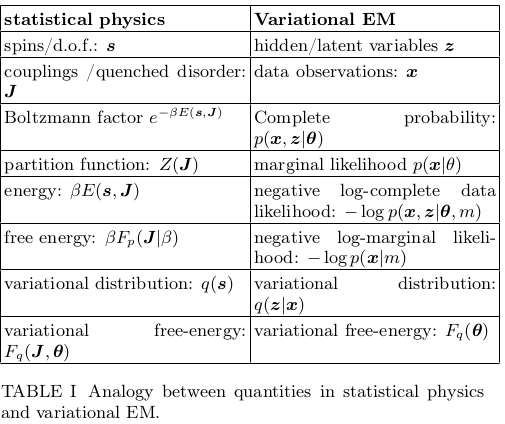
\includegraphics[width=0.7\linewidth]{gfx/AnalogyEMstatphys}
	\caption{}
	\label{fig:analogyemstatphys}
\end{figure}









\section{Energy Based Models: Maximum Entropy (MaxEnt) Principle, Generative Models, and Boltmann Learning}
\label{sec:energy}
\subsection{Introduction - Why do we need another class of models}
Supervised learning models discussed in \ref{ch:supervised} are \emph{discriminative} - they are designed to perceive differences between groups or categories of data. Discriminative models form the core techniques of most supervised learning methods, but they have several limitations.
\begin{enumerate}
	\item They require labelled data.
	\item There are tasks that discriminative approaches simply cannot accomplish, such as drawing new examples from an unknown probability distribution. 
\end{enumerate}

	A model that can earn to represent and sample from a probability distribution is called \emph{generative}. \emph{Energy-based} generative models are able to deal with tasks discriminative models even fail to attempt in the first place. This section is concerned with introducing these models.

\subsection{An overview of energy-based generative models}
\label{subsec:energyOverview}
\subsubsection{The idea}
This overview will highlight the similarities and differences with the supervised learning methods encountered in earlier sections.\\
\begin{mybox}{Generative model idea}
	Generative models are a ML technique that allows to learn how to generate new examples similar to those found in a training dataset. The core idea of most generative models is to learn a parametric model for the probability distribution from which the data was drawn. One we have learned a model, we can generate new examples by sampling from the learned generative model. As in stat. phys., this sampling is often done using MCMC methods.
\end{mybox}
The added complexity of learning models directly from samples introduces many of the same fundamental tensions we encountered when discussing discriminative models. The ability to generate new examples requires models to be able to "generalize" beyond the examples they have been trained on, that is to generate new samples that are not samples of the training set. The models must be expressive enough to capture the complex correlations present in the underlying data distribution, but the amount of data we have is finite which can give rise to overfitting.
\subsubsection{Generative models in practice}
In practice, most generative models that are used in ML are flexible enough that, with a sufficient number of parameters, they can approximate any probability distribution. For this reason,there are three axes on which we can differentiate classes of generative models:
\begin{enumerate}
	\item First axis is how easy the model is to train - both in terms of computational time and the complexity of writing code for the algorithm.
	\item The second axis is how well the model generalizes from the training set to the test set.
	\item The third axis is which characteristics of the data distribution the model is capable of and focuses on capturing.
\end{enumerate}
All generative models must balance these competing requirements and generative models differ in the tradeoffs they choose.\\
\\
One of the fundamental reasons that energy-based models have been less widely-employed than their discriminative counterparts is that the training procedure for these models differs significantly from those for supervised NNs (\ref{sec:dnn},\ref{sec:cnn},\ref{sec:dnn2}). Though both employ GD \ref{sec:gd} based procedure for minimizing a cost function (one common choice for generative models is the negative log-likelihood function \ref{eq:bayesErrorFct}), energy-based models do not use backpropagation\ref{subsec:dnnBackpropagation} and automatic differentiation for computing gradients. Rather, one must turn to ideas inspired by MCMC based methods in physics and statistics that sometimes go under the name "\emph{Boltzmann learning}". As a result, training energy-based models requires additional tools that are not immediately available in packages such as PyTorch and TensorFlow.\\
The open-source package \emph{Paysage} that is built on top of PyTorch bridges this gap by providing the toolset for training energy-based models. Paysage makes it easy to quickly code and deploy energy-based models such as Restricted Boltzmann Machines (RBMs) and Stacked RBMs - a "deep" unsupervised model.\\
\\
	Finally, we note that generative models at their most basic level are complex parametrizations of the probability distribution the data is drawn from. For this reason, generative models can do much more than just generate new examples. They can be used to perform a multitude of other tasks that require sampling from a complex probability distribution including "de-noising", filling in missing data, and even discrimination. The versatility of generative models is one of the major appeals of these unsupervised learning methods.


\subsection{Maximum entropy models: the simplest energy-based generative models}
\label{subsec:energyMaxEnt}
MaxEnt models have no latent (or hidden) variables, making them ideal for introducing the key concepts and tools that underlie energy-based generative models.
\subsubsection{Derivation of the theory}
It is possible to rederive the Boltzmann distribution (and the idea of generalized ensembles) entirely from information theoretic arguments. The Boltzmann distribution can be viewed as resulting from a statistical inference procedure for learning probability distributions describing physical systems where one only has partial information about the system (usually the average energy).\\
The key quantity in MaxEnt models is the information theoretic, or Shannon, entropy \ref{eq:infoShannon}. The Boltzmann distribution follows from the Principle of Maximum Entropy.
\begin{mybox}{Principle of Maximum Entropy}
A physical system should be described by the probability distribution with the largest entropy subject to certain constrains (often provided by measuring the average value of conserved, extensive quantities such as energy, particle number,..). The principle uniquely specifies a procedure for parametrizing the functional form of the probability distribution. Once we have specified and learned this form we can, of course, generate new examples by sampling this distribution.
\end{mybox}
How does this work ?\\
Suppose that we have chosen a set of functions $\{f_i(\mx)\}$ whose average value we want to fix to some observed values $\expval{f_i}_{obs}$. The Principle of Maximum Entropy states that we should choose the distribution $p(\mx)$ with the largest uncertainty (i.e. the largest Shannon entropy $S_p$ \ref{eq:infoShannon}), subject to the constraints that the model averages match the observed averages
\be 
\expval{f_i}_{model} = \int \md \mx f_i(\mx) p(\mx) = \expval{f_i}_{obs}.
\ee 
We can formulate the Principle of Maximum Entropy as an optimization problem using the method of Lagrange multipliers by minimizing 
\begin{align*}
	\mL[p] &= -S_p + \sum_i \lambda_i \left(\expval{f_i}_{obs} - \int \md \mx f_i (\mx) p(\mx) \right)\\
	&+ \gamma \left(1- \int \md \mx p(\mx)\right)\\
	0&=\frac{\delta \mL}{\delta p} = (\log p(\mx) +1) - \sum_i \lambda_i f_i(\mx) -\gamma,
\end{align*}
where the first set of constraints enforce the requirement for the averages and the last constraint enforces the normalization that the trace over the probability distribution equals one. The differentiation leads to the general form of the maximum entropy distribution
\be 
p(\mx) = \frac{1}{Z} e^{\sum_i \lambda_i f_i(\mx)}
\ee 
where $Z(\lambda_i)= \int \md \mx e^{\sum_i \lambda_i f_i(\mx)}$ is the partition function. The maximum entropy distribution is clearly just the usual Boltzmann distribution with energy $E(\mx) = - \sum_i \lambda_i f_i(\mx)$. The values of the Lagrange multipliers are chosen to match the observed averages for the set of functions $\{f_i(\mx)\}$ whose average value is being fixed:
\bse 
\expval{f_i}_{model}=\int \md \mx p(\mx) f_i(\mx) = \frac{\partial \log Z}{\partial \lambda_i} = \expval{f_i}_{obs}.
\ese 
In other words, the parameters of the distribution can be chosen such that 
\bse 
\partial_{\lambda_i} \log Z= \expval{f_i}_{data}.
\ese 
\begin{mybox}{Comparison to stat. phys.}
	Our $\mx$ denotes the microscopic state of the system, i.e. the MaxEnt distribution is a probability distribution over microscopic states. However, in thermodynamics we only have access to average quantities. If we know only the average energy $\expval{E(\mx)}_{obs}$, the MaxEnt procedure tells us to maximize the entropy subjet to the average energy constraints, this yields
	\be 
	p(\mx) = \frac{1}{Z} e^{-\beta E(\mx)},
	\ee 
	where we identified $\lambda_1 = - \beta= -1/k_BT$. Now suppose we also constrain the particle number $\expval{N(x)}_{obs}$. Then we obtain the following MaxEnt distribution
	\be 
	p(\mx) = \frac{1}{Z} e^{-\beta (E(\mx) - \mu N(\mx))},
	\ee 
	where we identified $\lambda_1=-\beta, \lambda_2=\mu/\beta$. Since this is just the Boltzmann distribution, we can also relate the partition function in our MaxEnt model to the thermodynamic free-energy via $F=-\beta^{-1} \log Z$. The choice of which quantities to constrain is equivalent to working in different thermodynamic ensembles.
\end{mybox}
\subsubsection{From statistical mechanics to ML}
The MaxEnt idea also provides a general procedure for learning a generative model from data. They key difference between MaxEnt models in physics and ML is that in ML we have no direct access to observed values $\expval{f_i}_{obs}$. Instead, these averages must be directly estimated from data (samples). To denote this difference, we will call empirical averages calculated from data as $\expval{f_i}_{data}$. We can think of MaxEnt as a statistical inference procedure simply by replacing $\expval{f_i}_{obs}$ by $\expval{f_i}_{data}$ as above.\\
This subtle change has important implications for training MaxEnt models. 
\begin{enumerate}
\item First, since we do not know these averages exactly, but must estimate them from the data, our training procedures must be careful not to overfit to the observations (our samples might no be reflective of the true values of these statistics). 
\item Second, the averages of certain functions $f_i$ are easier to estimate from limited data than others. This is often an important consideration when formulating which MaxEnt model to fit to the data.
\item Finally, we note that unlike in physics where conservation laws often suggest the functions $f_i$ whose averages we hold fix, ML offers no comparable guide for how to choose the $f_i$ we care about.
\end{enumerate}
For these reasons, choosing the $\{f_i\}$ is often farm from straightforward.\footnote{Note that MaxEnt is closely related to Bayesian inference from a ML perspective.}

\subsubsection{Generalized Ising models from MaxEnt}
The form of a MaxEnt model is completely specified once we choose the averages $\{f_i\}$ we wish to constrain. One common choice often used in MaxEnt modeling is to constrain the first two moments of a distribution. When our random variables $\mx$ are continuous, the corresponding MaxEnt distribution is a multi-dimensional Gaussian. If the $\mx$ are binary (discrete), then the corresponding MaxEnt distribution is a generalized Ising (Potts) model with all-to-all couplings.\\
\\
Partition functions for maximum entorpy models are often intractable to compute. Therefore, it is helpful to consider two special cases where $\mx$ has different support (different kinds of data). 
\begin{enumerate}
	\item First, consider the case that the random variable $\mx \in \mR^n$ are real numbers. The partition function can be calculated analytically
	\bse 
	Z = \int \md x e^{\mathbf{a}^T \mathbf{x}+\half \mathbf{x}^TJ\mx}=\sqrt{(2\pi)^n \det J^{-1}} e^{- \half \mathbf{a}^T J^{-1} \mathbf{a}}.
	\ese
	The resulting probability density function is,
	\begin{align}
		\label{eq:energyCostfctMaxEntmodel}
		p(\mx) &= Z^{-1} e^{-E(\mx)} =\frac{1}{\sqrt{(2 \pi)^n \det J^{-1}} } e^{\half \mathbf{a}^T J^{-1} \mathbf{a}+ \mathbf{a}^T \mx+ \half \mx^T J \mx }\nonumber \\
		&=\frac{1}{\sqrt{(2 \pi)^n \det \Sigma} } e^{-\half (\mx -\mu)^T \Sigma^{-1} (\mx-\mu)},
	\end{align} 
where $\mu=-J^{-1} \mathbf{a}$ and $\Sigma = - J^{-1}$. This, of course, is the normalized, multi-dimensional Gaussian distribution.
\item Second, consider the case that the random variable $\mx$ is a binary with $x_i \in \{-1,+1\}$. The partition function can no longer be computed in a closed form. This model is known as the Ising model in physics and as Markov Random Field in ML. Calculating partition function for the Ising model is intractable. For this reason, the best we can do is estimate it using numerical techniques such MCMC methods \todo{reference} or approximate methods like variational MFT methods \ref{sec:varMFT}. 
\end{enumerate}
Finally we note that ML and physics notation for binary variables differ ($x_i \in  \{0,1\}$ rather than $x_i \in \{\pm 1\}$), which can lead to confusion translating between literature or programming packages in ML and physics problems.





\subsection{Cost functions for training energy-based models}
\label{subsec:energyCostfctHowTo}
The MaxEnt procedure gives us a way if parametrizing an energy-based generative model.\\
	For any energy-based generative model, the energy function $E(\mx,\{\theta_i\} )$ depends on some parameters $\theta_i$ - couplings in the language of stat. phys.- that must be inferred directly from the data. For example, for the MaxEnt models the $\{\theta_i\}$ are just Lagrange multipliers $\{\lambda_i\}$. 
\begin{mybox}{Training procedure.}
The goal of the training procedure is to use the available training data to fit these parameters.\\
	Like in many other ML techniques, we will fit these couplings by minimizing a cost function using SGD \ref{subsubsec:gdSGD}. Such a procedure naturally separates into two parts: choosing an appropriate cost function, an calculating the gradient of the cost function with respect to the model parameters.
\end{mybox}
\begin{mybox}{Defining a cost function}
	 Formulating a cost function for generative models is a little bit trickier than for supervised, discriminative models. The objective of discriminative models is straightforward - predict the label from the features. However, what we mean by a "good" generative model is much harder to define using a cost function. We would like the model to generate examples similar to those we find in the training dataset. However, we would also like the model to generalize - we do not want the model to reproduce "spurious details" that are particular to the training dataset. Unlike for discriminative models, there is no straightforward idea like cross-validation on the data labels that neatly addresses this issue. For this reason, formulating cost functions for generative models is subtle and represent an important and interesting open are of research.
\end{mybox}
Calculating the gradients of energy-based models also turns out to be different than for discriminative models, such as DNNs. Rather than relying on automatic differentiation techniques and backpropagation, calculating the gradient requires drawing on intuitions from MCMC-baed methods.\\
\\
What follows is an in-depth discussion of \emph{Boltzmann learning} for energy-based generative models, focussing on MaxEnt models. We put the emphasis on training procedures that generalize to more complicated generative models with latent variables such as RBMs.






\subsubsection{Maximum likelihood}
By far the most common approach used for training a generative model is to maximize the log-likelihood of the training data set. Recall, that the log-likelihood characterizes the log-probability of generating the observed data using our generative model. By choosing the negative log-likelihood as the cost function, the learning procedure tries to find parameters that maximize the probability of the data.\\
In what follows, we employ a general notation that is applicable to all energy-based models, not just the MaxEnt models \ref{subsec:energyMaxEnt}. The reason for this is that much of this discussion does not rely on the specific form of the energy function but only on the fact that our generative model takes a Boltzmann form. We denote the generative model by the probability distribution $p_{\theta}(\mx)$ and its corresponding partition function by $\log Z(\{\theta_i\})$. In MLE, the parameters of the model are fit by maximizing the log-likelihood
\be 
\label{eq:energyCostfctLogLikely}
\mL(\{\theta_i\}) = \expval{\log(p_{\theta}(\mx))}_{data}=-\expval{E(\mx;\{\theta_i\})}_{data} - \log Z(\{\theta_i\}),
\ee 
where we made use of 
\begin{enumerate}
	\item Our generative distribution is of the Boltzmann form, and
	\item the partition function does not depend on the data
	\bse 
	\expval{Z}_{data}=Z.
	\ese 
\end{enumerate}


\subsubsection{Regularization}
\label{subsubsec:energyCostfctRegularization}
Just as for discriminative models like linear and logistic regression, it is common to supplement the log-likelihood with additional regularization terms (cf. \ref{subsec:lregRegularization}). Instead of minimizing the negative log-likelihood, one minimizes a cost function of the form
\be 
-\mL(\{\theta_i\}) +E_{reg}(\{\theta_i\}),
\ee 
where $E_{reg}(\{\theta_i\})$ is an additional regularization term that prevents overfitting. From a Bayesian perspective, this new term can be viewed as encoding a (negative) log-prior on model parameters and performing a maximum-a-posteriori (MAP) estimate instead of a MLE.
\begin{mybox}{Regularization energy based models}
	A common choice for the regularization function are the sums of the $L_1$ or $L_2$ norms of the parameters
	\be 
	\label{eq:energyCostfctRegularizationFct}
	E_{reg}(\{\theta_i\}) = \Lambda \sum_i \abs{\theta_i}^\alpha ,\quad \alpha=1,2
	\ee 
	with $\Lambda$ controlling the regularization strength. A large $\Lambda$ will force many parameters to be close to or exactly zero, $\Lambda=0$ is MLE. Just as in regression, an $L_1$ penalty enforces sparsity, with many of the $\theta_i$ set to zero, and $L_2$ regularization shrinks the size of the parameters towards zero.
\end{mybox}
One challenge of generative models is that is is often difficult to choose the regularization strength $\Lambda$. Recall that, for linear \ref{sec:linearRegression} and logistic regression \ref{sec:logisticRegression}, $\Lambda$ is chosen to maximize the out-of-sample performance on a validation dataset (i.e. cross-validation). However, for generative models our data are usually unlabelled. Therefore, choosing a regularization strength is more subtle and there exists no universal procedure for choosing $\Lambda$. One common strategy is to divide the data into a training set and a validation set and monitor a summary statistic such as the log-likelihood, energy distance, or variational free-energy \ref{subsubsec:varMFTEMphys} of the generative model on the training and validation sets. If the gap between the training and validation datasets starts growing, one is probably overfitting the model even if the log-likelihood of the training dataset is still increasing. This also give a procedure for "early stopping".\\
In practice, when using such regularizers it is important to try many different values of $\Lambda$ and then try to use a proxy statistic for overfitting to evaluate the optimal choice of $\Lambda$.



\subsection{Computing gradients}
\label{subsec:energyGradients}
We still need to specify a procedure for minimizing the cost function. SGD \ref{subsubsec:gdSGD} is normally employed, but how do you actually compute the gradients ?\\
Define operators conjugate to the parameters $\theta_i$
\bse 
\mO_i(\mx) = \frac{\partial E(\mx;\theta_i)}{\partial \theta_i},
\ese 
which implies, as $Z$ is the cumulant generating function for the Boltzmann distribution, that
\bse 
\expval{\mO_i(\mx)}_{model}= \tr_{\mx} p_{\theta}(\mx) \mO_i(\mx) = -\frac{\partial \log Z(\{\theta_i\})}{\partial \theta_i}.
\ese 
\begin{mybox}{MLE}
Then, \ref{eq:energyCostfctLogLikely} becomes
\begin{align}
	\label{eq:energyGradientsMLE}
	-\frac{\partial \mL(\{\theta_i\})}{\partial \theta_i} &= \langle \frac{\partial E(\mx;\theta_i)}{\partial \theta_i}\rangle_{data} +\frac{\partial \log Z(\{\theta_i\})}{\partial \theta_i} \nonumber \\
	&=\expval{\mO_i(\mx)}_{data} - \expval{\mO_i(\mx)}_{model}.
\end{align}
The gradient of the log-likelihood w.r.t. a model parameter \ref{eq:energyGradientsMLE} is a difference of moments - one calculated directly from the data and one calculated from our model using the current model parameters. The data-dependent term is known as the \emph{positive phase} of the gradient and the model-dependent term is known as the \emph{negative phase} of the gradient. This derivation also gives an intuitive explanation for likelihood-based training procedures. The gradient acts on the model to lower the energy of configurations that are near observed data points while raising the energy of configurations that are far from observed data points. Finally, we note that all information about the data only enters the training procedure through the expectations $\expval{\mO_i(\mx)}_{data}$ and our generative model is blind to information beyond what is contained in these expressions. 
\end{mybox}
\subsubsection{How does one actually compute the gradient then ?}
To use SGD, we must still calculate the expectation values in \ref{eq:energyGradientsMLE}. The positive phase of the gradient can be easily calculated using samples from the training dataset. The negative phase, however, is generally much more difficult to compute because analytically calculating the partition function is intractable for most interesting models.
\begin{definition}
	There are exceptional cases in which we can calculate the expectation values analytically. When this happens, the generative model is said to have a \emph{Tractable Likelihood}. One example of a generative model with a Tractable Likelihood is the Gaussian MaxEnt model for real valued data \ref{eq:energyCostfctMaxEntmodel}.
\end{definition}
Returning to the generic case where most energy-based model have \emph{intractable likelihoods}, we must estimate expectation values numerically. One way to do this is draw samples $\mathcal{S}_{model} =\{\mx^\prime_i\}$ from the model $p_{\theta}(\mx)$ and evaluate arbitrary expectation values using these samples:
\be 
\expval{f(\mx)}_{model} = \int \md \mx p_\theta(\mx) f(\mx) \approx \sum_{\mx^\prime_i\in\mathcal{S}_{model}} f(\mx^\prime_i).
\ee 
The samples from the model $\mx^\prime_i\in\mathcal{S}_{model}$ are often referred to as \emph{fantasy particles} in the ML literature and can be generated using simple MCMC algorithms such as Metropolis-Hasting.\\
\\
Finally, we note that once we have the fantasy particles from the model, we can also easily calculate the gradient of any expectation value $\expval{f(\mx)}_{model}$ using what is commonly called the "log-derivative trick" in ML
\begin{align*}
	\frac{\partial}{\partial \theta_i} \expval{f(\mx)}_{model} &= \int \md \mx \frac{\partial p_\theta(\mx)}{\partial \theta_i} f(\mx) \\
	&= \langle \frac{\partial \log p_\theta(\mx)}{\partial \theta_i} f(\mx)\rangle _{model} \\
&= \expval{\mO_i(\mx) f(\mx)}_{model} \approx \sum_{\mx^\prime_j\in\mathcal{S}_{model}} \mO_i(\mx_j) f(\mx^\prime_j).
\end{align*}




\subsection{Summary of the training procedure}
\label{subsec:energyTrainingProcedure}
We now summarize the discussion above and present a general procedure for training an energy-based model using SGD on the cost function.
\begin{mybox}{Training Procedure - Recipe}
	Our goal is to fit the parameters of a model $p_{\lambda}(\{\theta_i\}) = Z^{-1} e^{-E(\mx,\{\theta_i\})}$. Training the model involves the following steps:
		\begin{enumerate}
			\item Read a minibatch of data, $\{\mx\}$.
			\item Generate fantasy particles $\{\mx^\prime\} \sim p_\lambda$ using an MCMC algorithm (e.g., Metropolis-Hastings).
			\item Compute the gradient of log-likelihood using these samples and \ref{eq:energyGradientsMLE}, where the averages are taken over the minibatch of data nad the fantasy particles from the model, respectively.
			\item Use the gradient as input to one of the gradient based optimizers from \ref{sec:gd}.
		\end{enumerate}
\end{mybox}
\subsubsection{Practical tips}
In practice, it is helpful to supplement this pasigc proecure with some tricks that help training. As with discriminative NNs, it is important to initialize the parameters properly and print summary statistics during the training procedure on the traing and validation sets to prevent overfitting. This is more discussed in \ref{subsubsec:deepGenerativeTrainingPractical}\todo{Cheap tricks, to compile and reference !}.











\section{Deep Generative Models: Hidden Variables and Restricted Boltzmann Machines (RBMs)}
\label{sec:deepGenerative}
Here, we extend the discussion in \ref{sec:energy} to energy-based models that include latent or hidden variables.\\
Including latent variables in generative models greatly enhances their expressive power allowing the model to represent sophisticated correlations between visible veatures without sacrificing trainability.

\subsection{Why hidden (latent) variables ?}
\label{subsec:deepGenerativeWhy}
\subsubsection{Idea}
Latent or hidden variables are a powerful yet elegant way to encode sophisticated correlations between observable features.

\begin{mybox}{Quintessence - physics perspective}
	The underlying reason for this is that marginalizing over a subset of variables -"integrating out" degrees of freedom in the language of physics - induces complex correlations is a familiar component of many physical theories. For example when considering free electrons living on a lattice, integrating out phonons gives rise to higher-order electron-electron interactions (e.g. superconducting or magnetic correlations). More generally, in the Wilsonian renormalization group paradigm, all effective field theories can be though of as arising form integrating out high-energy degrees of freedom.
\end{mybox}
Generative models with latent variables run this logic in reverse.
\begin{mybox}{Quintessence - generative models perspective}
	Encode complex interactions between visible variables by introducing additional, hidden variables that interact with visible degrees of freedom in a simple manner, yet still reproduce the complex correlations between visible degrees in the data once marginalized over (integrated out). This allows us to encode interactions between the visible variables using simpler interactions at the cost of introducing new latent variables/degrees of freedom.
\end{mybox}
This trick is also widely exploited in physics (e.g. in the Hubbard-Stratonovich transformation or the introduction of ghost fields in gauge theory).

\subsubsection{For example - the Ising model}
\label{subsubsec:deepGenerativeHopfield}
To make these ideas more concrete, let us revisit the pairwise Ising model, which is described by a Boltzmann distribution $p(\mathbf{v}) = e^{E(\mathbf{v})}/Z$ with energy 
\bse 
E(\mathbf{v}) = - \sum_i a_i v_i - \half \sum_{ij} v_i J_{ij} v_j,
\ese 
where $J_{ij}$ is a symmetric coupling matrix that encodes the pairwise constraints and $a_i$ enforce the single-variable constraint.\\
Our goal is to replace the complicated interactions between the visible variables $v_i$ encoded by $J_{ij}$, by interactions with a new set of latent variables $h_\mu$. In order to do this, it is helpful to rewrite the coupling matrix in a slightly different form. Using SVD, we can always express the coupling matrix in the form $J_{ij} = \sum_{\mu=1}^N W_{i \mu} W_{j\mu}$, where $\{W_{i\mu}\}$ are appropriately normalized singular vectors.
\begin{mybox}{Hopfield model}
	 In terms of $W_{i\mu}$, the energy takes the form
\be 
\label{eq:deepGenerativeHopfield}
E_{Hop}(\mathbf{v}) = -\sum_i a_i v_i - \half \sum_{ij \mu} v_i W_{i \mu} W_{ j\mu} v_j.
\ee 
We note that in the special case when both $v_i \in \{-1,+1\}$ and $W_{i\mu} \in \{-1,+1\}$ are binary variables, a model with this form of the energy functions is known as the \emph{Hopfield model}.
Note that here we will refer to all energy functions of the form\ref{eq:deepGenerativeHopfield} as (generalized) Hopfield models, even for the case when the $W_{i\mu}$ are continuous variables.
\end{mybox}
We now "decouple" the visible variables $v_i$ by introducing a set of normally, distributed continuous latent variables $h_\mu$ such that we can rewrite the Boltzmann distribution for the generalized Hopfield model as
\begin{align*}
	p(\mathbf{v}) &= \frac{e^{\sum_i a_i v_i+\half \sum_{ij\mu} v_i W_{i\mu} W_{j\mu} v_j} }{Z}\\
		&= \frac{e^{\sum_i a_i v_i} \prod_\mu \int \md h_\mu e^{-\half \sum_\mu h^2_\mu-\sum_i v_i W_{i\mu} h_\mu} }{Z} \\
		&\equiv \frac{\int \md \mathbf{h}e^{-E(\mathbf{h,v}) }}{Z},
\end{align*}
where $E(\mathbf{v,h})$ is a joint energy functional of both the latent and visible variables of the form
\be 
E(\mathbf{v,h}) = - \sum_i a_i v_i + \half \sum_\mu h^2_\mu - \sum_{i\mu} v_i W_{i\mu} h_\mu. 
\ee 
We can also use the energy function $E(\mathbf{v,h})$ to define a new energy-based model $p(\mathbf{v,h})$ on both the latent and visible variables
\be 
p(\mathbf{v,h}) = \frac{e^{-E(\mathbf{v,h}) }}{Z^\prime}.
\ee 
Marginalizing over latent variables of course gives us back the generalized Hopfield model
\be 
p(\mathbf{v}) =\int \md \mathbf{h}p(\mathbf{v,h}) = \frac{e^{-E_{Hop}(\mathbf{v})}}{Z}.
\ee 
Notice that $E(\mathbf{v,h})$ contains no direct interactions between visile degrees of freedom (or between hidden degrees of freedom). Instead, the complex correlations between the $v_i$ are encoded in the interaction between the visible $v_i$ and latent variables $h_\mu$. It turns out that the model presented here is a special case of a more general class of powerful energy-based models called Restricted Boltzmann Machines (RBMs).


\subsection{Restricted Boltzmann Machines (RBMs)}
\label{sec:deepGenerativeRBM}


\begin{figure}[h!]
	\centering
	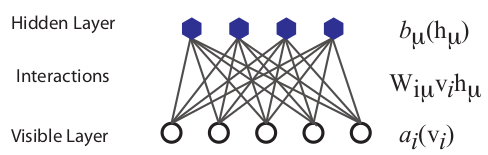
\includegraphics[width=0.5\linewidth]{gfx/RBM}
	\caption{\itshape A RBM consists of visible units $v_i$ and hidden units $h_\mu$ that interact with each other through interactions of the form $W_{i\mu}v_ih_\mu$. Importantly, there are no interactions between visible units themselves or hidden units themselves.}
	\label{fig:RBM}
\end{figure}

\begin{mybox}{RBM}
	A RBM is an energy-based model with both visible and hidden units where the visible and hidden units interact with each other but do not interact among themselves, compare figure \ref{fig:RBM}. The energy function of an RBM takes the general functional form
	\be 
	\label{eq:deepGenerativeRBMenergy}
	E(\mathbf{v,h}) = - \sum_i a_i (v_i) -\sum_\mu b_\mu (h_\mu) - \sum_{i\mu} W_{i\mu} v_i h_\mu,
	\ee 
	where $a_i(\cdot)$ and $b_\mu(\cdot)$ are functions that we are free to choose. The most common choice is:
		\bse 
a_i(v_i) = \Bigg\{
\begin{array}{ll}
	a_i v_i& \text{if $v_i\in \{0,1\}$ is binary}\\
	\frac{v^2_i}{2 \sigma^2_i}, & \text{if $v_i\in \mR$ is continuous}.
\end{array}
\ese 
		and,
		\bse 
		b_\mu(h_\mu) =\Bigg\{ \begin{array}{ll}
			b_\mu h_\mu & \text{if $h_\mu \in \{0,1\}$ is binary}\\
			\frac{h^2_\mu}{2 \sigma^2_\mu}, & \text{if $h_\mu\in \mR$ is continuous}.
	\end{array}
	\ese 
	For this choice of $a_i,b_\mu$, layers consisting of discrete binary units are often called \emph{Bernoulli layers}, and layers consisting of continuous variables are often called Gaussian layers.
\end{mybox}
The different possible combinations are the following.\\
 \begin{tabular}{|l|ll|}
	       Name &Visible Layer $a_i(v_i)$ & Hidden Layer $b_\mu(h_\mu)$ \\
	\toprule
"RBM" & Bernoulli & Bernoulli\\
Multi-dimensional Gaussian & Gaussian &Gaussian \\
Generalized Hopfield model& Bernoulli &Gaussian \\
Gaussian Bernoulli RBM & Gaussian &Bernoulli\\
	\bottomrule
\end{tabular}
\vspace{0.1cm}
Specifying a generative model with this bipartite interaction structure has two major advantages:
\begin{enumerate}
\item It enables capturing both pairwise \emph{and higher-order} correlations between the visible units and 
\item it makes it easier to sample from the model using an MCMC method known as block Gibbs sampling, which in turn makes the model easier to train.
\end{enumerate}

\subsubsection{Content of an RBM}
We want to understand the kind of correlations that can be captured using an RMB.\\
One can derive that the marginal energy includes all order of interactions between the visible units, with the $n$-th order cumulants of the distribution of hidden units $q_\mu(h_\mu) = e^{b_\mu(h_\mu)}/Z$ weighting the $n$-th order interactions between the visible units.\\
This exemplifies the incredible representational power of RBMs with a Bernoulli hidden layer. Each hidden unit can encode interactions of arbitrarily high order. By combining many different hidden units, we can encode very complex interactions at all orders. Moreover, we can learn which order of correlations/interactions are important directly from the data instead of having to specify them ahead of time as we did in the MaxEnt models \ref{subsec:energyMaxEnt}. This highlights the power of generative models with even the simplest interactions between visible and latent variables to encode, learn, and represent complex correlations present in the data.



\subsection{Training RBMs}
\label{subsec:deepGenerativeTraining}
RBMs are a special class of energy-based generative models, which can be trained using the MLE procedure described in detail in \ref{subsec:energyGradients},\ref{subsec:energyTrainingProcedure}. The gradient (SGD) can be calculated using \ref{eq:energyGradientsMLE}. As before calculating the negative phase of the gradient (i.e. the expectation value w.r.t. to the model) requires that we draw samples from the model. The bipartite form of the interactions in RBMs were specifically chosen with this in mind.

\subsubsection{Gibbs sampling and contrastive divergence (CD)}
\label{sububsec:deepGenerativeTrainingGibbsCD}
The bipartite interaction structure of an RBM makes it possible to calculate expectation values using a MCMC method known as Gibbs sampling. The key reason for this is that since there are no auto-interactions in the layers, the visible and hidden units of an RBM are conditionally independent:
\begin{align}
	\label{eq:deepGenerativeTrainingGibbsCDdistributions}
	p(\mathbf{v} |\mathbf{h}) &= \prod_i p(v_i|\mh),\; p(\mh|\mv) = \prod_\mu p(h_\mu|\mv) \nonumber \\
	p(v_i|\mh) &=\sigma(a_i +\sum_\mu W_{i\mu} h_\mu) \\
	p(h_\mu =1 |\mv) &= \sigma(b_\mu + \sum_i W_{i\mu} v_i)\nonumber,
\end{align}
and where $\sigma(z)=1/(1+e^{-z})$ is the sigmoid function.\\
\begin{mybox}{Procedure}
	Using these expressions it is easy to compute expectation values w.r.t. the data. The input to GD is a minibatch of observed data. For each sample in the minibatch, we simply clamp the visible units to the observed values and apply \ref{eq:deepGenerativeTrainingGibbsCDdistributions} using the probability for the hidden variables. We then average over all samples in the minibatch to calculate expectation values w.r.t. the data. To calculate expectation values w.r.t. the model, we use (block) Gibbs sampling. The idea behind (block) Gibbs sampling is to iteratively sample from the conditional distribution $\mh_{t+1} \sim p(\mh |\mv_t)$ and $\mv_{t+1} \sim p(\mv|\mh_{t+1})$. Since the units are conditionally independent, each step of this iteration can be performed by simply drawing random numbers. The samples are guaranteed to converge to the equilibrium distribution of the model in the limit that $t\rightarrow$. At the end of the Gibbs sampling procedure, one ends up with a minibatch of samples (fantasy particles).
\end{mybox}
To create a guaranteed independent sample, one resorts to using an approximate Gibbs sampling technique called \emph{Contrastive Divergence}(CD). In CD-$n$, we just perform $n$ interations of (block) Gibbs sampling, with $n$ often taken to be as small as $1$, it has proven to work reasonably well. Furthermore, to introduce stochasticity into the drawn dataset one uses a variant called Persistent CD (PCD). In PCD, rather than restarting the Gibbs sampler from the data at each GD step, we start the Gibbs sampling at the fantasy particles in the last GD step. Since parameters change slowly compared to the Gibbs sampling, samples that are high probability at one step of the SGD are also likely to be high probability at the next step. This ensures that PCD does not introduce large errors in the estimation of the gradients. The advantage of using fantasy particles to initialize the Gibbs sampler is to allow PCD to explore parts of the feature space that are much further from the training dataset than one could reach with ordinary CD, thus creating a randomized and independent minibatch via stochasticity.

\subsubsection{Practical Considerations}
\label{subsubsec:deepGenerativeTrainingPractical}
Important tricks in the application are the following.
\begin{enumerate}
	\item \emph{Initialization}.\\
	The model must be initialized. Hinton suggests taking the weights $W_{i\mu}$ from a Gaussian with mean zero and standard deviation $\sigma=0.01$. An alternative initialization scheme proposed by Glorot and Bengio instead chooses the standard deviation to scale with the size of the layers: $\sigma = 2/\sqrt{N_v+N_h}$ where $N_v$ and $N_h$ are number of visible and hidden units respectively. The bias of the hidden units is initialized to zero while the bias of the visible units is typically taken to be inversely proportional to the mean activation, $a_i=\expval{v_i}^{-1}_{data}$.
	\item \emph{Regularization}.\\
	One can of course use an $L_1$ or $L_2$ penalty, typically only on the weight parameters, not the biases. Alternatively, Droput has been shown to decrease overfitting when training with CD and PCD, which results in more interpretable learned features.
	\item  \emph{Learning rates}.\\
	Typically, it is helpful to reduce the learning rate in later stages of training.
	\item \emph{Updates for CD and PCD}.\\
	There are several computational tricks one can use for speeding up the alternating updates in CD and PCD, linked in Hinton $2012$.
\end{enumerate}




\subsection{Deep Boltzmann Machine}
\label{subsec:deepGenerativeDBM}
\subsubsection{The idea}
Unlike RBMs, DBMs possess multiple hidden layers and were the first models rebranded as "deep learning".
Basically, you stack RBMs, the idea is the following.\\
First of all we note the quintessential properties of RBMs again and their shortcomings.\\
An RBM is composed of two layers of neurons that are connected via an undirected graph \ref{fig:RBM}. As a result, it is possible to perform sampling $\mathbf{v}\sim p(\mathbf{v|h})$ and inference $\mh \sim p(\mh|\mv)$ with the same model. As with the Hopfield model \ref{eq:deepGenerativeHopfield}, we can view each of the hidden units as representative of a pattern, or feature, that could be present in the data.\footnote{In general, one should instead think of activity patterns of hidden units representing features in the data.} The inference step involves assigning a probability to each of these features that expresses the degree to which each featue is present in a given data sample. In an RBM, hidden units do not influence each other during the inference step, i.e. hidden unit are conditionally independent given the visible units. How can we create connections between the hidden units ? This is essentially what a DBM boils down to.
\begin{mybox}{DBM idea}
	For a DBM, you stack multiple RBMs together to generate intra-layer interactions. How do we do this ?\\
	With the Hopfield model, we saw that pairwise lienar connections between neurons can be mediated through another layer. Therefore, a simple way to allow for effective connections between the hidden units is to add another layer of hidden units. Rather than just having two layers, one visible and one hidden, we can add additional layers of latent variables to account for the correlations between hidden units. Ideally, as one adds more and more layers, one might hope that the correlations between hidden variables become smaller and smaller deeper into the network. This basic logic is reminiscent of renormalization procedures that seek to decorrelate layers at each step.
\end{mybox}
The price of adding additional layers is that the models become harder to train.
\subsubsection{Training a DBM}
\label{subsubsec:deepGenerativeDBMTraining}
Training DBMs is more subtle than RBMs due to the difficulty of propagating information from visible to hidden units. Some of these problems can be alleviated via a layer-wise procedure.\\
Rather than attempting to train the whole DBM at once, we can think of the DB; as a stack of RBMs, compare figure \ref{fig:dbm}.
\begin{mybox}{Training procedure}
	One first trains the bottom two layers of the DBM - treating it as if it is a stand-alone RBM. Once this bottom RBM is trained, we can generate "samples" from the hidden layer and use these samples as an input to the next RBM (consisting of the first and second hidden layer - purple hexagons and green squares in Fig. \ref{fig:dbm}). This procedure can then be repeated to pretrain all layers of the DBM.
\end{mybox}
This pretraining initializes the weights so that SGD can be used effectively when the network is trained in a supervised fashion. In particular, the pretraining helps the gradients to stay well-behaved rather than vanish or blow up (cf. \ref{subsubsec:dnnBackpropagationProblems}).\\
It is worth noting that once pretrained, we can use the usual Boltzmann learning rules in \ref{eq:energyGradientsMLE} to fine-tune the weights and improve the performance of the DBM. As we demonstrate in the following, the Paysage packaged can be used to both construct and train DBMs using such a pretraining procedure.





\begin{figure}[h!]
	\centering
	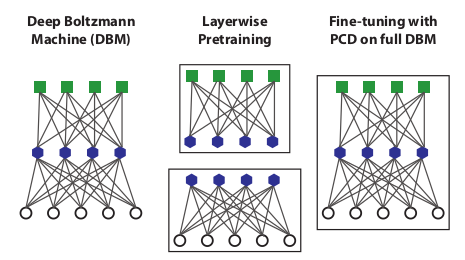
\includegraphics[width=0.7\linewidth]{gfx/DBM}
	\caption{\itshape Deep Boltzmann Machine contain multiple hidden
		layers. To train deep networks, first we perform layerwise
		training where each two layers are treated as a RBM. This
		can be followed by fine-tuning using gradient descent and per-
		sistent contrastive divergence (PCD).}
	\label{fig:dbm}
\end{figure}








































 
\chapter{Topic to work on}
\section{Temporal/Sequential Data}
What are techniques for dealing with temporal or sequential data. A powerful class of models for sequential data called Hidden Markov Models that utilize dynamical programming techniques have natural statistical physics interpretations in terms of transfer matrices. Recently, Recurrent NNs (RNNs) have become an important and powerful tool for dealing with sequence data. RNNs generalize many of the ideas discussed in \ref{sec:dnn} to deal with temporal data.
\section{Reinforcement learning}
Many of the most exciting developments in the last five years have come from combining reinforcement learning with DNNs. RL traces its origins to behaviourist psychology, when it was conceived as a way to explain and study reward-based decision making. RL is a field of ML, in which an angent learns how to master performing a specific task through an interaction with its environment. Depending on the reward it receives, the agent chooses to take an action affecting the environment, which in turn determines the value of the next received reward, and so on. The long-term goal of the agent is to maximize the cumulative expected return, thus improving its performance in the longer run.

\section{Support Vector Machines (SVMs) and Kernel Methods}
SVMs and kernel methods are a powerful set of techniques that work well when the amount of training data is limited.
























\chapter{Philosophical discussion of intelligence and consciousness}
AI, by design, is an ambiguous term that mixes aspirations with reality. It also conflates the statistical ideas that form the basis of modern ML with the more commonplace notions about what humans and behavioural scientists mean by intelligence. See \href{https://arxiv.org/abs/1604.00289}{Lake et al.} for an enlightening and important modern discussion of this distinction from a quantitative cognitive science point of view as well as \href{https://www.rand.org/pubs/papers/P3244.html}{Dreyfus} for a surprisingly relevant philosophy-based critique from $1965$.\\
\\
Almost all the techniques discussed here rely on optimizing a pre-specified objective function on a given dataset. Yet, we know that for large, complex models changing the data distribution or the goal can lead to an immediate degradation of performance. Deep networks have poor generalizations to even a sightly different context (the infamous Validation-Test set mismatch). This inability to abstract and generalize is a common criticism lobbied against branding modern ML techniques as AI (See Lake).\\
\\
The "Singularity" may not be coming but the advances in computing and the availability of large data sets likely ensure that the kind of statistical learning frameworks discussed are here to stay. Rather than a AGI, the kind of techniques presented here seem to be best suited for three important tasks:
\begin{enumerate}
	\item Automating prediction from lots of labelled examples in a narrowly-defined setting,
	\item learning how to parametrize and capture the correlations of complex probability distributions, and
	\item finding policies for tasks with well-defined goals and clear rules.
\end{enumerate}



\chapter{Social implication of ML}
Caution is in order when applying ML. Without foresight and accountability, the scale and scope of modern ML algorithms can lead to large scale unaccountable and undemocratic outcomes that can reinforce or even worsen existing inequality and inequities.\footnote{See book: O’Neil, Cathy (2017), Weapons of math destruction: How big
	data increases inequality and threatens democracy (Broad-
	way Books).}
When ML is used in a social context, abstract statistical relationships have real social consequences. False positives can mean the difference between life and death (e.g. signature drone strikes). ML algorithms, like al techniques, have important limitations and should be employed with great caution.\\
All algorithms involve inherent tradeoffs in fairness, \href{https://arxiv.org/abs/1609.05807}{see}. It is farm from clear how to make algorithms fair for all people involved. This is even more true with methods like DL that are hard to interpret. All ML algorithms have implicit assumptions and choices reflected in the datasets we use to the kind of functions we choose to optimize. It is important to remember that there is no "view from nowhere", compare \href{https://course.ccs.neu.edu/cs5150f14/readings/adam-artificialknowing.pdf}{1} and \href{https://papers.ssrn.com/sol3/papers.cfm?abstract_id=3078224}{2} - all ML algorithms reflect a point of view and a set of assumptions about the world we live in.








\chapter{Ideas for problems to work on}
\section{Physics problems}
\subsection{Cosmology}
\begin{enumerate}
	\item Maybe write a classification logistic regressor, or deep CNN to classify where dark matter halos have their boundary. It is very difficult to define a boundary of such a spread out object with confidence, maybe find criteria via classification ML technique ?
\item Maybe use density contrast concept from cosmology for density based clustering \ref{subsubsec:clusterPracticalDBSCAN}. Basically a mean field approach ?
\end{enumerate}
\subsection{QFT}
\begin{enumerate}
	\item Connected correlation functions describe n-point correlations between points (like covariance matrix). Can maybe find a motivation of describing connected correlations from qft, how do you infer connected correaltions from dataset ? Then you can find the set of one, two and higher n-point corr. functions for one class in your data, i.e. the ones which are correlated (inter cluster correlation possible ?Should be, compare \ref{fig:hierarchicalclustering}). Need to Wick rotate to Euclidean space for analogy. Can one use Feynman diagrams ?\\
	This should be interesting since you normally would consider relative ratios of probabilities for highly-complex unsupervised learning tasks as described in \ref{sec:varMFT}. The same is done in QFT, where you have cumulants which are normalized such that the partition function cancels out, i.e. we do not need to know the whole configuration.
	\item How can one infer distance and curvature from a picture. If i do a panorama picture, the points in the middle are further away (which is encoded in their curvature) and the ones on the side are rather far (at least the ones in the middle are squished), how can you generally tell curvature ? Can you construct a pixel triangle and infer local curvature from it or do you first need to find a metric in the local manifold describing the dataset locally ?
	\item Rather than understanding clusters as different densities  \ref{subsubsec:clusterPracticalDBSCAN} one could think of clusters like disconnectd (or maybe even connected if correlated ?) patches of a manifold. How can you fin the parametrization of this manifold, how its intrinsic metric and how the embedded metric ? Look at \href{https://arxiv.org/pdf/1802.03426.pdf}{manifold link}.
\end{enumerate}
\section{Ai safety}
\subsection{Questions}
\begin{enumerate}
	\item Can you define multiple hierarchical utility functions to implement Asimov's laws via reinforcement learning ?
\end{enumerate}
\section{Knobel-problems}
\subsection{Ideas}
\begin{enumerate}
	\item Write a CNN which looks at a Sudoku picture, converting it into a Sudoku data grid, then solve it via python ?
	
\end{enumerate}
\section{ML questions}
Is it possible to reconstruct the analytic representation of the function found by an agent to approximate the data we are interested in ?
What is the question here. First of all, normally we propose a model class to approximate the data in supervised learning problems. Using NN or unsupervised learning concepts, one however does not know the model class, one does not know the latent variables describing your problem. These agents readjust their weights and biases until the data is accurately represented or approximated. Could one translate this idea of weights and biases into an analytic function or model of functions ?\\
Could one use this to model the behaviour of a physical system, approximate the function and then let it be analytically represented to back-engineer the physical model describing the system ?
\end{document}
% ********************************************************************
